%pleiades.jpeg --- CC BY 2.0 Solar Anamnesis; modified attribution, Carsten Frenzl from Deutschland, CC BY 2.0, via Wikimedia Commons or Flickr: https://flic.kr/p/2oeBmbN.
\documentclass[a4paper, 11pt, oneside]{article}
\usepackage{kmath, kerkis}
\usepackage[T1]{fontenc}
% Load encoding definitions (after font package)
\usepackage{textalpha}

\usepackage[dvipsnames]{xcolor}
\usepackage{eso-pic,graphicx}
\usepackage[top=45mm, bottom=45mm, outer=29mm, inner=29mm]{geometry}
\setlength{\columnsep}{90pt}

% Babel package:
\usepackage[main=german,polutonikogreek]{babel}
\usepackage{listings}
\lstset{basicstyle=\ttfamily}

% With XeTeX$\$LuaTeX, load fontspec after babel to use Unicode
% fonts for Latin script and LGR for Greek:
\ifdefined\luatexversion \usepackage{fontspec}\fi
\ifdefined\XeTeXrevision \usepackage{fontspec}\fi

% "`Lipsiakos"' italic font `cbleipzig`:
\newcommand*{\lishape}{\fontencoding{LGR}\fontfamily{cmr}%
		       \fontshape{li}\selectfont}
\DeclareTextFontCommand{\textli}{\lishape}

\usepackage{sectsty}
\usepackage[titles]{tocloft}

\sectionfont{\Huge}
\subsectionfont{\LARGE}
\subsubsectionfont{\Large}

\usepackage{setspace}
\onehalfspacing

\usepackage{booktabs}
\usepackage{graphicx}
\setlength{\emergencystretch}{15pt}
\graphicspath{ {./ } }
\usepackage[figurename=]{caption}
\usepackage{float}
\usepackage{fancyhdr}
\usepackage{microtype}

% change color of text, example replace all \color{Goldenrod} with \color{lightgray}

\makeatletter % change only the display of \thepage, but not \thepage itself:
\patchcmd{\ps@plain}{\thepage}{\bfseries\large\color{SkyBlue}{\thepage}}{}{}
\makeatother

\color{SkyBlue}

\begin{document}
\bfseries
\pagestyle{plain} % after changing a pagestyle command, it's necessary to invoke it explicitly
\AddToShipoutPictureBG{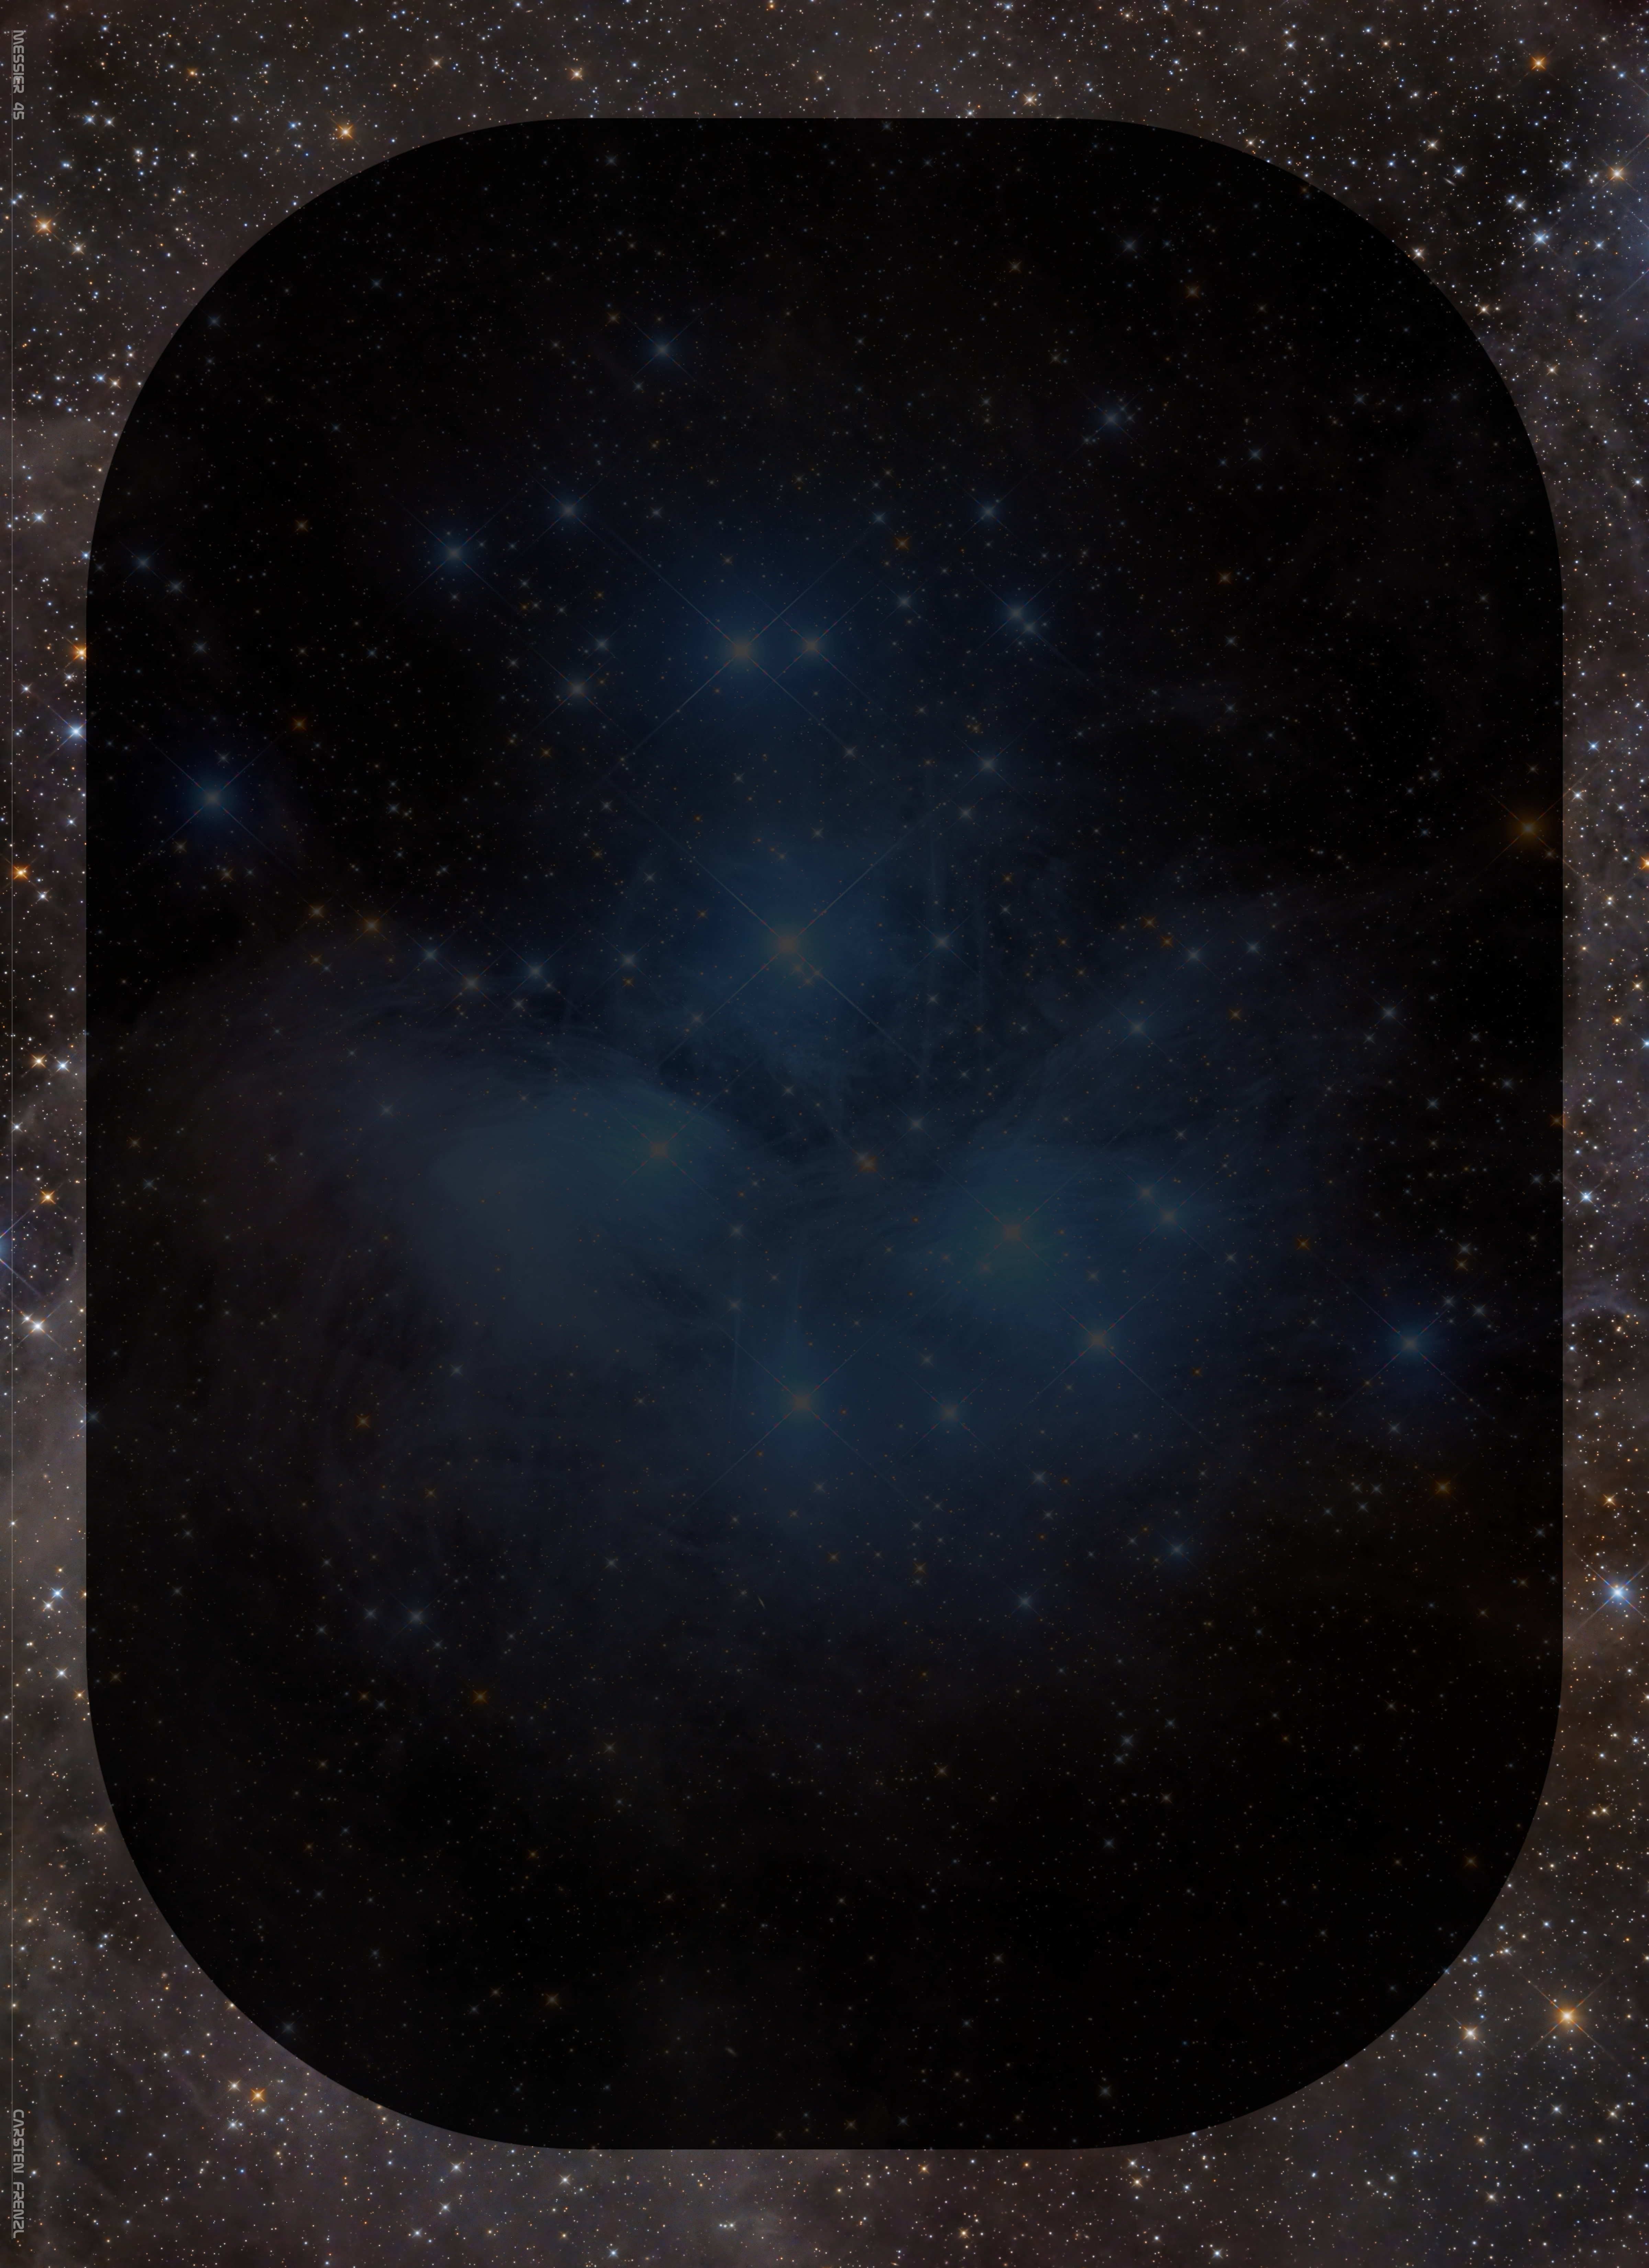
\includegraphics[width=\paperwidth,height=\paperheight]{pleiades.jpeg}}

\renewcommand\thefootnote{{\bfseries\color{SkyBlue}{\arabic{footnote}}}}
\let\oldfootnote\footnote
    \renewcommand{\footnote}[1]{\oldfootnote{{\normalsize\bfseries\color{SkyBlue}#1}}}
\begin{titlepage} % Suppresses headers and footers on the title page
	\centering % Centre everything on the title page
	%\scshape % Use small caps for all text on the title page

	%------------------------------------------------
	%	Title
	%------------------------------------------------
	
	\rule{\textwidth}{1.6pt}\vspace*{-\baselineskip}\vspace*{2pt} % Thick horizontal rule
	\rule{\textwidth}{0.4pt} % Thin horizontal rule
	
	\vspace{1\baselineskip} % Whitespace above the title
	
	{\scshape\Huge Nektar und Ambrosia}
	
	\vspace{1\baselineskip} % Whitespace above the title

	\rule{\textwidth}{0.4pt}\vspace*{-\baselineskip}\vspace{3.2pt} % Thin horizontal rule
	\rule{\textwidth}{1.6pt} % Thick horizontal rule
	
	\vspace{1\baselineskip} % Whitespace after the title block
	
	%------------------------------------------------
	%	Subtitle
	%------------------------------------------------
	
	{\scshape \Large Mit einem Anhang über die Grundbedeutung der Aphrodite und Athene} % Subtitle or further description
	
	\vspace*{1\baselineskip} % Whitespace under the subtitle

        {\scshape Von \Large Dr. Wilhelm Heinrich Roscher,\\\normalsize Professor und Konrektor am Kgl. Gymnasium zu Wurzen}

	\vspace*{4\baselineskip} % Whitespace under the subtitle

        \begin{quotation}
        \centering
        
        Οἱ μὲν οὖν περὶ Ἡσίοδον καὶ πάντες... θεολόγοι... τὰ μὴ γευσάμενα τοῦ νέκταρος καὶ τῆς ἀμβροσίας θνητὰ γενέσθαι φασίν, δῆλον ὡς ταῦτα τὰ ὀνόματα γνώριμα λέγοντες αὑτοῖς.
        
        \scshape Aristot. Met. 2, 4
        \end{quotation}

        %------------------------------------------------
	%	Editor(s)
	%------------------------------------------------
        \vspace*{\fill}

	\vspace{1\baselineskip}

	{\small\scshape Leipzig 1883}
	
	{\small\scshape{Druck und Verlag von B. G. Teubner}}
 
	\vspace{0.5\baselineskip} % Whitespace after the title block

        \scshape Internet Archive Online Edition  % Publication year
	
	{\scshape\small Namensnennung Nicht-kommerziell Weitergabe unter gleichen Bedingungen 4.0 International} % Publisher
\end{titlepage}
\setlength{\parskip}{1mm plus1mm minus1mm}
\clearpage
\vspace*{\fill}
\begin{center}
\LARGE
ΤΗΙ ΦΙΛΟΞΕΝΩΙ ΕΛΛΑΔΙ

Ο ΣΥΓΓΡΑΦΕΥΣ

ΑΝΕΘΗΚΕΝ
\end{center}
\vspace*{\fill}
\clearpage
\Large
\tableofcontents
\clearpage
\section*{Übersicht des Inhalts.}
\subsection*{Vorbemerkungen.}
\paragraph{}
Über Aufgabe und Methode meiner mythologischen Untersuchungen. Ziel: die Ermittlung der Naturbasis eines Mythenkomplexes und des Zusammenhanges aller einzelnen darin enthaltenen mythischen Anschauungen und Funktionen. Methode: Vergleichung sämtlicher im Mythus und Kultus vorhandenen Vorstellungen mit den von den Alten an ein bestimmtes Naturobjekt geknüpften Anschauungen und Nachweis ähnlicher oder gleicher Ideen bei andern verwandten und nicht verwandten Völkern. Über die Beziehungen des Hermes zum Winde nebst Nachträgen zu meiner Monographie "`Hermes der Windgott."' Ähnlich sollen in der nachstehenden Untersuchung die Beziehungen des Nektars und der Ambrosia zum Honig nachgewiesen werden. Über den Deutungsversuch des Porphyrios und Bergks. Kurze Übersicht über die gewonnenen Resultate.

\subsection*{Kapitel 1.}

\subsubsection*{A.}

\textbf{\emph{Der Honig fällt nach antikem Glauben als Tau vom Himmel oder aus der Luft auf die Pflanzen (Bäume und Blumen) nieder und gilt demnach für eine Art von Himmelsspeise. Ähnliche Vorstellungen bei den Hebräern (Manna), Indern, Germanen und Finnen.}}

Griechen und Römer hielten den Honig für eine Art Tau, der vom Himmel oder aus der Luft auf die Pflanzen niederfalle. Dies erklärt sich aus der Erscheinung des sogenannten, "`Honigtaus,"' d. i. eines honigartigen Saftes, welchen die Blätter der Pflanzen bisweilen ausschwitzen. Verschiedene Benennung des "`Honigtaus"' bei den Alten (ἀερόμελι, δροσόμελι, ἄγριον oder ὗον μέλι). Besonders werden Eichen, Rohrarten, Eschen (μελίη hängt wohl mit μέλι zusammen) vom Honigtau befallen. Die Vorstellung von den honigtriefenden Eichen des goldenen Zeitalters. Die Manna der Bibel, eine besondere Art des Honigtaus, als Himmelsspeise und tauähnlicher Honig bezeichnet. Berichte griechischer Schriftsteller über mannaähnliche Erscheinungen an europäischen und asiatischen Bäumen. Auch der Blumenhonig wurde als Tau aufgefasst. Zeugnisse des Hesiod, Aristoteles, Vergil u. s. w. Nachweis gleicher Vorstellungen von der Entstehung des Honigs bei den Indern, Germanen und Finnen. Die honigträufelnde Weltesche Yggdrasil.

\subsubsection*{B.}

\textbf{\emph{Ambrosia = Götterspeise, Nektar = Göttertrank und umgekehrt. Diese Vertauschung der beiden Ausdrücke erklärt sich aus deren ursprünglicher Identität, insofern beide nur verschiedene Formen derselben Substanz (des Honigs) waren. Die homerische Sage von den Ambrosia bringenden Peleiai (Pleiaden).}}

In den homerischen Gedichten bezeichnet ἀμβροσίη in der Regel die Speise, νέκταρ den Trank der Götter; daneben bestand freilich noch eine entgegengesetzte Tradition (Alkman, Sappho \emph{etc.}), wonach νέκταρ die Speise, ἀμβροσία den Trank der Götter bedeutet. Diese sonderbare Vertauschung der beiden Ausdrücke erklärt sieh einfach aus der Annahme, dass νέκταρ und ἀμβροσία ursprünglich nur verschiedene Formen derselben Substanz, des Honigs, waren, welcher nicht bloß als Speise, sondern (in verdünntem Zustande) auch als Trank (Meth) betrachtet werden konnte. Etymologie des Wortes νέκταρ (= νώγαλον). Honigtau und Blumenhonig entstehen nur im Sommer, zwischen dem Auf- und Untergang der Pleiaden. So entstand der Mythus von den Πέλειαι oder Πελειάδες, welche dem neugeborenen Zeus aus dem Göttergarten des äußersten Westens Ambrosia bringen. Nach einer andern Tradition soll Zeus von Bienen mit Honig ernährt worden sein. Wenn Ambrosia auch als Futtergras der Götterrosse erscheint, so beruht dies wohl auf einer Übertragung des Begriffes Unsterblichkeitsnahrung von den Göttern auf ihre Rosse.

\subsection*{Kapitel 2.}

\subsubsection*{A.}

\textbf{\emph{Der Honig als Speise, berauschendes Getränk, Salbe und Reinigungsmittel.}}

Honig als Speise bald rein, bald mit andern Substanzen gemischt genossen. Honig zur Bereitung eines berauschenden Getränkes (Meth) vor der Einführung des Weinbaues benutzt. Hydromeli und Melikraton. Dionysos ursprünglich vielleicht ein Gott des Honigmethes, weshalb ihm die Erfindung des Honiggenusses zugeschrieben wurde. Honig als Salbe und als Reinigungsmittel (ῥύμμα).

\subsubsection*{B.}

\textbf{\emph{Ambrosia-Nektar als Speise, Trank, Salbe und Reinigungsmittel.}}

Die homerischen Stellen, an denen Ambrosia als Salbe und Reinigungsmittel erscheint. Anderweitige Zeugnisse.

\subsection*{Kapitel 3.}

\subsubsection*{A.}

\textbf{\emph{Süßigkeit, Lieblichkeit and Wohlgeruch des Honigs.}}

\subsubsection*{B.}

\textbf{\emph{Süßigkeit, Lieblichkeit und Wohlgeruch der Ambrosia und des Nektars.}}

\subsection*{Kapitel 4.}

\subsubsection*{A.}

\textbf{\emph{Der Genuss des Honigs macht die Menschen gesund und verlängert das Leben. Heilkraft des Honigs.}}

Die Ansicht der Pythagoreer und des Demokritos von der gesundheitsfördernden Wirkung des Honigs. Zeugnisse des Plinius Galenos, Hippokrates u. A. Honig als Arzneimittel. Legende von Sol als dem Entdecker der heilenden Kraft des Honigs. Die verschiedenen Leiden, welche durch Honig geheilt wurden. Honig als Wundsalbe in einem finnischen Liede.

\subsubsection*{B.}

\textbf{\emph{Ambrosia und Nektar machen die Götter unsterblich. Heilkräfte derselben.}}

Widerlegung von Bergks Ansicht, dass die Unsterblichkeit der Götter nicht auf dem Genüsse von Nektar und Ambrosia beruhe. Die entgegenstehenden Zeugnisse der Alten. Ambrosia als Wundsalbe. Nektar als belebendes und stärkendes Getränk.

\subsection*{Kapitel 5.}

\subsubsection*{A.}

\textbf{\emph{Erhaltende (antiseptische) Wirkung des Honigs. Honig als Einbalsamierungmittel.}}

Antiseptische Wirkung des Honigs. Honig als Einbalsamierungmittel bei den Babyloniern und spartanischen Königen. Anderweitige Zeugnisse für die Einbalsamierung der Leichen bei den Griechen. Honig zum Einlegen der Früchte und zum Konservieren animalischer Substanzen benutzt.

\subsubsection*{B.}

\textbf{\emph{Erhaltende (antiseptische) Wirkung der Ambrosia. Ambrosia als Einbalsamierungmittel.}}

Thetis schützt die Leiche des Patroklos durch Einträufeln von Ambrosia und Nektar in die Nase vor Verwesung. Auch die Ägypter flößten ihren Toten antiseptische Substanzen durch die Nase ein. Sarpedon durch Salbung mit Ambrosia vor Verwesung geschützt. Der homerische Ausdruck ταρχύω = ταριχεύω weist auf uralte Einbalsamierungsitte auch bei den Griechen.

\subsection*{Kapitel 6.}

\subsubsection*{A.}

\textbf{\emph{Honig in derselben Bedeutung wie sonst Ambrosia und Nektar als Götterspeise, als Opferspeise, als Totenopfer und erste Nahrung menschlicher und göttlicher Kinder.}}

Die alten Zeugnisse für den Glauben der Griechen, dass Honig die Nahrung der Götter sei. Ambrosia von Dichtern wie Ibykos als 9- oder 10fache Potenz des Honigs bezeichnet. Honig als erste Nahrung neugeborener Menschen- und Götterkinder. Ähnlicher Brauch bei den Indern, Germanen und Hebräern. Honig als Opferspeise der Götter. Honig als Totenopfer.

\subsubsection*{B.}

\textbf{\emph{Ambrosia und Nektar in der Bedeutung von μέλι gebraucht. Ambrosia und Nektar als Nahrung der neugeborenen Götterkinder.}}

Zeugnisse für den Gebrauch von ἀμβροσία und νέκταρ = μέλι. Zeugnisse für den Glauben der Alten an die Ernährung neugeborener Götterkinder mit Nektar und Ambrosia.

\subsection*{Kapitel 7.}

\subsubsection*{A.}

\textbf{\emph{Μέλι in metaphorischem Gebrauche von der Süßigkeit der Rede und des Gesanges.}}

Vergleich süßer Rede mit süßem Honig. μέλι in der Bedeutung von Gesang. Vergleich des Dichters mit einer Biene. Legende von Komatas.

\subsubsection*{B.}

\textbf{\emph{Νέκταρ in übertragener Bedeutung von der Süßigkeit des Gesanges.}}

Belege aus den alten Dichtern.

\subsection*{Schlussbemerkungen.}

Widerlegung der Ansicht, dass der Wein das ursprüngliche Substrat des Nektars sei. Die Übersicht über den Inhalt des Anhangs s. auf S. 107.
\clearpage
\section*{Vorbemerkungen.}
\paragraph{}
Bereits in zwei früher erschienenen Monographien "`Hermes der Windgott"' (1878) und "`die Gorgonen und Verwandtes"' (1879) habe ich den Versuch gemacht größere Gruppen scheinbar wenig oder gar nicht miteinander zusammenhängender mythologischer Vorstellungen mittelst einer selbständigen Methode auf eine gemeinsame Naturbasis zurückzuführen und damit zugleich bis ins feinste Detail hineinzuerklären. Dabei ergab sich gleichzeitig ungesucht eine vielfach merkwürdige Übereinstimmung uralter griechischer Vorstellungen mit denjenigen anderer verwandter Völker, namentlich der Inder, Italiker und Germanen. So ließen sich die sämtlichen Funktionen des Hermes mit leichter Mühe und ziemlicher Evidenz auf die Vorstellungen der Alten vom Winde, die Prädikate und Funktionen der Gorgonen dagegen auf die verschiedenen der Anschauung des Gewitters entsprungenen Ideen zurückführen, welche teils aus den Etymologien der zur Bezeichnung der betreffenden Vorstellungen gebrauchten Ausdrücke, teils aus den älteren Dichtern und den Werken der antiken Naturforscher und Philosophen gewonnen wurden. Wie dies zu verstehen ist möge das Beispiel des Hermes lehren, dessen Mythus scheinbar aus lauter unvereinbaren Funktionen und Vorstellungen zusammengesetzt ist.

Die Bedeutung, welche Hermes als Diener der Götter, namentlich des Zeus hatte, erklärt sich einfach aus der das ganze Altertum, namentlich aber den Homer und die übrigen Dichter beherrschenden Anschauung, dass der Wind das Werkzeug der Götter, besonders aber des Zeus sei und von diesem gesendet werde (vgl. Ζεὺς εὐάνεμος, οὔριος, \emph{Juppiter auctor tempestatum}, Διὸς οὖρος, ἦλθ' ἄνεμος Ζέφυρος μέγας, αἴθριος ἐκ Διὸς αἴσης, ἐπὶ δὲ Ζεὺς τερπικέραυνος ὦρσεν ἀπ' Ἰδαίων ὀρέων ἀνέμοιο θύελλαν u. s. w.)

Wie die Winde in der Regel aus dem Äther oder den Wolken oder von den Gipfeln der Berge niederfahren\footnote{Dieselbe Vorstellung hat neuerdings Lenormant bei den Chaldäern nachgewiesen: Magie und Wahrsagekunst der Chaldäer. S. 28.} und --wegen des beständig darin herrschenden Luftzuges --- in Berghöhlen (Windhöhlen)\footnote{In meinem Hermes S. 20 f. habe ich unterlassen zu erwähnen, dass die Kyllenische Höhle, in welcher H. geboren sein sollte, höchst wahrscheinlich eine sogen. Windhöhle war. Cornelius Meteorologie S. 232 sagt darüber: "`Die Windhöhlen oder Wetterlöcher, meist in höheren Gebirgen vorkommend, sind durch kalte Luftströmungen charakterisiert, die aus ihnen mit größerer oder geringerer Heftigkeit hervorbrechen. Häufig finden sich die Windhöhlen in Italien, so am Monte Testaccio zu Rom, auf der Insel Ischia, am Hügel bei San Marino, im Monte Eolo bei Terni... bei Chiavenna und bei Caprino unweit Lugano. Die meiste Beachtung unter ihnen fand die Höhle des Monte Eolo, deren Eingang ein altes verfallenes Thor schließt, durch dessen Spalten der Wind mit vielem Getöse heraus bläst... Im Sommer bläst kalte Luft aus dem Berge heraus, umgekehrt verhält es sich im Winter, wo die äußere Luft in die Höhle hineinzieht. [Hy. in Merc. 146 f.] Bei den meisten andern Windhöhlen hat man Gleiches beobachtet."' Vgl. Sen. Nat. Q. 5, 14, 1: Repetam nunc, quod primo dixeram, edi e specu ventos recessuque anteriore terrarum. Der "`Ebe"' ist ein trockener warmer Wind, von dem die Kirgisen und Tataren meinen, dass er aus verborgenen Grotten ströme. Hamm im Ausland 1878. S. 764. Vielleicht hängt die Idee des Ἑρμῆς καταχθόνιος hiermit zusammen. Stengel macht im Hermes 1881. S. 349 f. darauf aufmerksam, dass die Opfer an die Winde gleich Opfern an die unterirdischen Gottheiten und an die Toten gehalten worden sind.} wohnend gedacht werden (vgl. Ausdrücke wie Βορέας αἰθρηγενής, ἐκνεφίας, ἐπαΐσσειν Διὸς ἐκ νεφελάων, ἐπαιγίζειν ἐξ αἰθέρος, καταιγίζειν, κατιέναι, Ῥιπαῖα ὄρη, ἑπτάμυχον Βορέαο σπέος u. s. w.), so ist Hermes, der Sohn des Äthergottes Zeus und der Regenwolkennymphe Μαῖα (Πλειάς = lat. \emph{pluvia}), entweder auf dem Olymp oder in der Höhle der Kyllene, d. i. des Hohlberges (vgl. Κυλλήνη mit lat. \emph{caelum}), worunter man ursprünglich wohl den hohlen Wolkenberg verstand,\footnote{Von der Verwandtschaft der Begriffe "`Wolke"' und "`Berg"' handelt ausführlich Schwartz, Die poet. Naturanschauungen 2 (1879) S. 13 ff. Vgl. auch Lucr. 6, 159 u. 189. In Betreff der \emph{cavae nubes} s. Sen. Q. Nat. 2, 27, 4. Plin. n. h. 2, 133. Lucr. 6, 176. 195. 202. 272.} geboren.

Den an Schultern und Füssen beflügelten Winden (Boreaden)\footnote{Vgl. auch Stephani, Boreas und die Boreaden, Petersburger Akademie. 1871. S. 6. 12. 15. 21. Wackernagel ΕΠΕΑ ΠΤΕΡΟΕΝΤΑ S. 6.} vergleicht sieh der an Schultern oder Füssen beflügelte Hermes, wie jene, so wird auch dieser zugleich als schnell, gewandt und kraftvoll\footnote{Nachzutragen Hermes S. 33: Xen. Hell. 5, 4, 17. Sen. Q. Nat. 2, 22, 2. 5, 13, 3. Gell. N. A. 2, 22, 29.} gedacht (vgl. die Ausdrücke ἲς ἀνέμοιο, ἀνέμων μένος, βίαι ἀνέμων, \emph{ventus validus}, \emph{violentus}, Βορέης κραιπνός, Βορέης αἰψηροκέλευθος, ἀνέμων σπέρχωσιν ἄελλαι, ταχύπτεροι πνοαί, πνοαὶ ὑψιπετᾶν ἀνέμων, Ἑ. Διὸς ἄλκιμος υἱός u. s. w.). Hiermit hängt die Funktion des Hermes als Gottes der Gymnastik und Agonistik zusammen.

Der sehr verbreiteten Vorstellung von dem Stehlen, Rauben und Betrügen der Winde (ἀνέλοντο θύελλαι, ἄρπυιαι ἀνηρείψαντο, ἀνήρπασε θέσπις ἄελλα, \emph{aurae fallaces}, \emph{petulantes}, \emph{venti protervi}, ἄνεμος ἀσελγής, ὑβριστής, ἀνέμοις παραδοῦναί τι u. s. w.)\footnote{Nachzutragen S. 39: Sen. Q. Nat. 5, 13, 3: Hinc fere omnia pericula venti erupti de nubibus prodeunt, quibus armenta rapiantur et totae naves in sublime tollantur. ib. 2, 22, 2: Videamus, quantis procellae viribus ruant, quanto vertantur impetu turbines. id quod obvium fuit, dissipatur et rapitur et longe a loco suo proicitur. Liv. 21, 58, 7: nec quod statutum esset manebat omnia perscindente vento et rapiente, Od. θ 408: ἔπος δ' εἴ πέρ τι βέβακται || δεινόν, ἄφαρ τὸ φέροιεν ἀναρπάξασαι θύελλαι u. Ameis z. d. St. Xen. Hell. 5, 4, 17. Vgl. auch Schwartz, Poet. Naturanschauungen 2, 53. Πολίτης, δημώδεις μετεωρ. μῦθοι Athen. 1880. S. 43.} entspricht der diebische, trügerische Charakter des Gottes, der unter Anderm auch als Entführer der Götterrinder (Wolken) auftritt.

Wie die Winde überall als göttliche Pfeifer und Sänger auftreten --- ich erinnere an die Mythen der Maruts, des Vaju und des Wodan und berufe mich auf Ausdrücke wie Ζεφύροιο ἰωή, ἠχή,\footnote{Nachzutragen S. 50: Hes. Theog. 708: ἄνεμοι... φέρον δ' ἰαχήν τ' ἐνοκήν τε. S. 52, Anm. 201: Sen. Q. Nat. 2, 28, 3 ventus... sibilat. Schwartz a. a. O. 59.} κεκληγῶς Ζέφυρος, ἄνεμος λιγύς, λιγυρός, βύκτης, συρίζων, σύριγμα ἀνέμων, \emph{ventus susurrans}, \emph{aura sibilans} u. s. w. --- so gilt Hermes zunächst als Erfinder des αὐλός und der σῦριγξ, als der einfachsten Blasinstrumente, und sodann auch der Lyra.

Auch die Psychopompie des Hermes lässt sich leicht auf seine ursprüngliche Bedeutung als Windgott zurückführen, wenn man bedenkt, dass die Seelen (ψυχαί, \emph{animae}) von jeher luftartig gedacht wurden und demnach bei der Trennung vom Körper in das Reich des Windes oder der Luft, der sie entstammen, zurückkehren müssen.\footnote{Zu S. 58: Auch die Abchasen halten die Seelen für luftartig. Die Seelen derjenigen, deren Leichname nicht haben gefunden werden können, werden auf eigentümliche Weise in Schläuchen gefangen und dann bestattet. Ausland 1880. S. 1019 f. Noch der moderne Grieche flucht: ἄγε εἰς ἄνεμον, πήγαινε εἰς ἂν. Schwartz, Ursprung d. Myth. 30, 2. Vgl. auch Πολίτης, δημώδεις μετεωρολογικοὶ μῦθοι Athen. 1880. S. 44 f.}

Wie die Seelen scheinen aber auch die ihnen nahe verwandten Traumbilder aus der Luft zu stammen und den Schlafenden vom Winde zugeführt zu werden (vgl. Redensarten wie εἴδωλον σταθμοῖο παρὰ κληῖδα λιάσθη ἐς πνοιὰς ἀνέμων; ὄνειρος ist verwandt mit ἄνεμος): darum ist Hermes zugleich Seelenführer und Traumgott oder Schlafgott geworden.\footnote{Zu S. 64 f.: Ap. Rh. 4, 877: αὐτὴ (Thetis) δὲ πνοιῇ ἰκέλη δέμας ἠύτ' ὄνειρος βῆ ῥ' ἵμεν ἐκ μεγάρονο. Il. \emph{B}, 71: ἀποπτάμενος ὄνειρος. Zu S. 66: In Betreff der Gleichsetzung von Seelen und Träumen ist nachzutragen Porphyr de antro n. 28: δῆμος δὲ ὀνείρων κατὰ Πυθαγόραν αἱ ψυχαί, ἃς συνάγεσθαί φησιν εἰς τὸν γαλαξίαν. Von der Verwandtschaft des Hermes mit Hypnos handelt G. Krüger in Jahrb. f. kl. Philol. 1863. S. 289 f. Vgl. auch Brunn in den Annali d. inst. 1868. S. 351 ff.}

Da ferner die Winde dem Ackerbauer und Hirten bald fruchtbare Regenwolken (ὄμπνιον νέφος Soph. fr. 233 D.) bald trockenes Wetter bringen und daher vielfach als befruchtend\footnote{Zu S. 72 ff.: Geopon. 2, 26, 1: πεπαινομένου τοῦ καρποῦ ὑπό τε τῶν ἀνέμων καὶ τῆς ἄλλης τοῦ ἀέρος εὐκρασίας, Mehr bei Hamm im Ausland 1878. S. 763 ff.} und zugerisch gedacht werden (vgl. Ζεφυρίη πνείουσα τὰ μὲν φύει, ἄλλα δὲ πέσσει, \emph{genitabilis aura}, \emph{Favonius}, ἀὴρ πυροφόρος, ἔγχος ἀνεμοτρεφές u. s. w.) und sogar nach einem von Aristoteles und Plinius bezeugten Hirtenglauben die Befruchtung der Heerden hauptsächlich vom Winde abhängt,\footnote{Vgl. auch Aelian, nat. an. 7, 27.} so gilt Hermes als δώτωρ ἐάων und ἐριούνιος, als Verleiher des Heerdenreichtums und Hirtengott und wird oft phallisch dargestellt. Auch als Förderer der Gesundheit wurde er verehrt, weil die Winde oft die Luft von schädlichen Miasmen reinigen und dadurch Krankheiten abwehren oder mindern.\footnote{Vgl. Hamm im Ausland 1878. S. 763. Auch Rudra, der Sturmgott, wirkt wohltätig, indem er die Luft von Miasmen reinigt. Kaegl. Zürcher Programm v. 1878. S. 24 f.}

Weil der Wind wegen seiner Launenhaftigkeit und Unbeständigkeit\footnote{Vgl. Caes. de bello civ. 3, 26, 5 u. 27, 1. Plut. mor. p. 95 B: οἱ τῶν πράξεων καιροὶ καθάπερ τὰ πεύματα τοῖς μὲν φέρουσιν τοῖς δὲ ἀποπίπτουσιν.} von jeher und überall als ein Sinnbild des Glückes angesehen wurde, so ist Hermes als Windgott auch zu einem Gotte des plötzlich und unerwartet eintretenden Glückes und Zufalls geworden, dem deshalb auch die Glücksruthe und die Loose geheiligt waren.

Sehr einfach erklärt sich die Funktion des Hermes als Gottes der Wege und der Wanderer aus seiner ursprünglichen Windbedeutung, wenn man bedenkt, dass Reisende vorzugsweise von Wind und Wetter abhängig sind.\footnote{Zu S. 87, Anm. 327 ist noch hinzuzufügen: Xen. Hell. 5, 4, 17. Plut. de prim. frig. 18. Arrian Anab. 1. 26, 1. Liv. 21, 58, 4. Goethe Ges. Werke. 1840. 23, 6. Der Windgott wurde auch selbst als Wanderer gedacht: Schwartz, Poet. Naturanschauungen 2, 70 f.}

Die uralten Namen und Beinamen Ἀργειφόντης (= ἀργέστης), διάκτορος und Ἑρμείας enthalten ebenfalls noch deutliche Beziehungen zum Winde, ebenso die Verehrung des Gottes am vierten Monatstage, weil an diesem nach uraltem Volksglauben Wind und Wetter wechseln, ferner das Symbol des Hahnes, eines das Wetter vorausahnenden und durch seinen Ruf prophezeienden Tieres,\footnote{Zu S. 101. Anm. 391: Demokritos bei Plut. de san. p. 14: Ἄτοπον γάρ ἐστι... κλωσμοῖς ἀλεκτορίδων... ὡς ἔφη Δημόκριτος, ἐπιμελῶς προσέχειν, σημεῖα ποιουμένους πνευμάτων καὶ ὄμβρων.} und die Sage von der Geburt des Hermes am frühen Morgen, da der Wind, welcher den Tag über weht, sich in der Regel schon mit Sonnenaufgang erhebt.

Endlich findet sich vielfache Übereinstimmung des Hermes mit andern anerkannten Windgöttern indogermanischer Völker, namentlich mit Wodan, Vaju und den Maruts.

Zu meiner großen Freude ist nun nicht bloß das Resultat, sondern auch die Methode, welche zu demselben geführt hat, ziemlich allgemein anerkannt worden,\footnote{Vgl. Schweizer-Sidler in Fleckeisens Jahrb. 1879. S. 309 ff. Bursian in der Jenaer Literaturzeitung. 1879. S. 425 ff. Conze in d. Archaeol. Zeitg. 1880. S. 8. Trendelenburg ebenda. 1880. S. 132. Literar. Centralbl. 1879. S. 1225. Der einzige Gelehrte, welcher bisher Widerspruch erhoben hat, ist E. v. Schmidt in seiner Schrift "`Die Philosophie d. Mythologie v. Max Müller."' Berlin. 1880. S. 71 ff. Derselbe hält Hermes für einen Lichtgott, welche Annahme sich aber, wie ich an einem andern Orte gelegentlich auszuführen gedenke, leicht als völlig unhaltbar erweisen lässt.} so dass ich hoffen darf, dieselbe werde sich im Laufe der Zeit mehr und mehr einbürgern und noch manches ähnliche Ergebnis zu Tage fördern. Dass in der Tat noch viele mythologische Probleme mittels jener einfachen Methode sich lösen lassen, möge die nachstehende Untersuchung lehren, deren Zweck es ist die sämtlichen Vorstellungen, welche die Alten vom Nektar und von der Ambrosia hatten, auf das Substrat des Honigs zurückzuführen.

Auf absolute Neuheit kann dieser Gedanke freilich keinen Anspruch machen. Schon Porphyrios in seiner Schrift de antro nympharum 16 sagt: ὅθεν τινὲς (vielleicht sind hierunter frühere Pythagoreer zu verstehen, da, wie wir sehen werden, der Honig von den sämtlichen Anhängern des Pythagoras sehr geschätzt wurde) ἠξίουν τὸ νέκταρ καὶ τὴν ἀμβροσίαν, ἣν κατὰ ῥινῶν στάζει ὁ ποιητὴς εἰς τὸ μὴ σαπῆναι τοὺς τεθνηκότας, τὸ μέλι ἐνδέχεσθαι, θεῶν τροφῆς ὄντος τοῦ μέλιτος.\footnote{Gemeint ist die Konservierung der Leiche des Patroklos durch Thetis, welche dem Toten durch die Nase Nektar und Ambrosia einflößt.} Man hielt also schon im Altertum aus zwei Gründen den Honig mit Nektar und Ambrosia für identisch, einmal wegen seiner konservierenden, gewissermaßen unsterblich machenden, Kraft und zweitens weil er geradezu ebenso wie Nektar und Ambrosia für eine Götterspeise galt (vgl. z. B. Hy. in Merc. 560. Batrachom. 39).

In neuerer Zeit haben sich für eine Beziehung zwischen Honig und Nektar und Ambrosia, soviel ich weiß, nur zwei Forscher, W. Menzel und Th. Bergk, ausgesprochen. Ersterer hat in seiner lesenswerten Monographie über die Biene (Mythologische Forschungen und Sammlungen Bd. 1. Stuttgart 1842) ganz kurz und ohne irgend näher auf die Sache einzugehen die Vermutung geäußert, dass die Vorstellung von Nektar und Ambrosia auf dem Substrat des Honigs beruhen dürfte. Viel ausführlicher hat dagegen Th. Bergk die Frage nach dem ursprünglichen Wesen des Nektars and der Ambrosia behandelt in einem besonderen Kapitel seines überaus anregenden und geistreichen, freilich aber auch zugleich viele schiefe und unhaltbare Behauptungen enthaltenden Aufsatzes "`Über die Geburt der Athene,"' welcher im sechsten Jahrgang der von Fleckeisen herausgegebenen Jahrbücher für klassische Philologie 1860 S. 289 ff. und 377 ff. erschienen ist. Bergk geht darin S. 316 (Kap. 6) von der Ansicht aus, dass nach dem ältesten Glauben der Nektar ein Wasser sei, welches einem himmlischen Quell oder See entspringe.\footnote{Vgl. S. 388: "`Ursprünglich ist Nektar oder Ambrosia, den der heilige Quell Trito spendet, nichts anderes als das reine himmlische Wasser."'} Dieses himmlische Wasser, welches den Trank der Götter bilde, ohne sie jedoch unsterblich zu machen (S. 377 f.), sei bald Nektar bald Ambrosia genannt worden; wo beide Ausdrücke neben einander erschienen "`ist die angemessenste Erklärung überall die, dass man annimmt, die allgemeine Bedeutung sei auch hier wie so oft mit einer spezielleren verbunden, um den Begriff vollständig zu erschöpfen, ungefähr wie man πρὸς ἠῶ τ' ἠἑλιόν τε, οὐρανὸς Οὔλυμπός, und ähnliches verbunden findet"' (S. 380). Noch in der Ilias sei nur von einem Göttertranke, nirgends von einer Götternahrung die Rede, Ambrosia dagegen bezeichne entweder das Salböl oder das Futter der Götterrosse; das Verbum στάζω, was mehrfach auch mit ἀμβροσίην verbunden werde (Il. \emph{T.} 38. 347. 354), spreche für die Identität von Nektar und Ambrosia, insofern Beides eine flüssige nicht feste Substanz bezeichne (S. 378 u. 379). Ein wirklicher Unterschied zwischen beiden Ausdrücken im Sinne von Speise und Trank trete erst Od. ε. 93 hervor. Bergk meint, dass diese Unterscheidung auf einem späteren Missverständnis des formelhaften Hendiadyoin νέκταρ τε καὶ ἀμβροσίην ἐρατεινήν (S. 380). Jene ältere Anschauung aber, die nur einen Göttertrank kenne, der mit verschiedenen Namen bald Nektar bald Ambrosia benannt worden sei, trete noch in der bei Alkman, Sappho und Anaxandrides vorkommenden Verwechselung der beiden Ausdrücke deutlich hervor (S. 381). Später habe man sich gewöhnlich den Nektar (welcher ursprünglich nach Bergk, wie schon gesagt, ein himmlisches Trinkwasser bedeutete) als eine Art Wein vorgestellt, wie aus den Verbindungen νέκταρ οἰνοχοεύειν, κεράσαι, νέκταρ ἐρυθρόν hervorgehe, diese Vorstellung sei natürlich erst nach der Einführung des Weinbaues bei den Hellenen aufgekommen, während man vor dieser Zeit, als noch der Honigmeth das beliebteste Getränk der Hellenen gewesen sei, sich auch den Nektar als eine Art Meth vorgestellt habe. Spuren der älteren Sitte hätten sich noch in den sogenannten νηφάλια und im Hymnus auf Hermes 5. 562, wo der Honig als θεῶν ἡδεῖα ἐδωδή bezeichnet werde, erhalten (S. 382 f.)

Dies die Ansicht Bergks hinsichtlich der Entstehung der Vorstellungen von Nektar und Ambrosia. Wir werden im Verlaufe unserer Untersuchung die einzelnen Behauptungen Bergks oft genug zu kritisieren und zu widerlegen haben, daher wir hier auf eine eingehende Beurteilung verzichten dürfen. Nur so viel mag hier gesagt sein, dass Bergk weder eine einigermaßen vollständige Materialsammlung gegeben hat noch auch, trotz seiner richtigen Ahnung von einem einstigen Zusammenhang des Nektars und der Ambrosia mit dem Honig, zu einem methodischen Beweise gelangt ist. Der Grund davon liegt wohl in seiner verkehrten und durchaus unerweislichen Annahme, dass Nektar und Ambrosia noch bei Homer fast stets identisch seien und im Grunde nur das "`himmlische Wasser"' bedeuteten.\footnote{Auf dieser falschen Deutung beruht wohl auch die sonderbare Ton mir in Kap. 4, B. mit bestimmten Zeugnissen widerlegte Annahme Bergks, dass die Alten dem Genuss von Nektar und Ambrosia keine unsterblichmachende Wirkung zugeschrieben hätten.} So sanken für ihn die Beziehungen, welche der Meth einstmals zum Göttertranke gehabt haben muss, nur zu untergeordneter Bedeutung herab, er untersucht sie weder genau noch gibt er sie vollständig an, er begnügt sich damit, einige dürftige Spuren einstiger Beziehung des Methes zum Göttertranke nachgewiesen zu haben, welche für ihn kaum mehr Interesse besitzen, als die späteren Beziehungen des Nektars zum Weine.

Das Resultat meiner eigenen Untersuchungen lässt sich kurz folgendermaßen darstellen.

Nach dem Glauben der Griechen und Römer war der Honig eine Art Tau, welcher vom Himmel oder aus der Luft auf die Pflanzen (Bäume und Blumen) niederfiel und von den Bienen gesammelt wurde. Diese Annahme erklärt sich einfach aus der Erscheinung des sogenannten "`Honigtaus,"' d. i. eines honigartigen Saftes, welchen die Blätter der Bäume auf der der Sonne zugekehrten Seite nicht selten ausschwitzen. Wie wir von einem "`Honigtau"' so redeten schon die Alten von ἀερόμελι, δροσόμελι, ἄγριον oder ὗον μέλι, \emph{rores mellei} Plin. \emph{aërium mel} Verg. Besonders wurden Eichen, gewisse Rohrarten und Eschen vom Honigtau befallen. Der Name der Esche μελίη hängt also wohl mit μέλι Honig zusammen. So erklärt sich die Vorstellung von den honigtriefenden Eichen des goldenen Zeitalters. Eine besondere Art des Honigtaus scheint die Manna der Bibel gewesen zu sein, auch sie wird zugleich dem Tau und dem Honig verglichen und als Himmelsspeise bezeichnet. Endlich wurde auch der Blumenhonig, wie aus Zeugnissen des Hesiodos, Aristoteles, Vergilius hervorgeht, als ein himmlischer Tau aufgefasst. Dieselben Vorstellungen von der Entstehung des Honigs sind bei den Indern, Germanen und Finnen nachweisbar. Man denke nur an die honigträufelnde Weltesche Yggdrasil der nordischen Mythologie. Auch diesen Völkern erscheint demnach der Honig schon seiner Herkunft wegen als eine süße Himmelsspeise (Kap. 1, A.)

Bei Homer bezeichnet ἀμβροσίη in der Regel die Speise, νέκταρ den Trank der Götter. Nach einer andern Tradition, welche von Alkman, Sappho und dem Komiker Anaxandrides vertreten wird und jedenfalls auch sehr alt ist, weil sie sich sonst schwerlich gegenüber der in diesen Dingen maßgebenden Autorität des Homer hätte behaupten können, bezeichnet νέκταρ die Speise, ἀμβροσία den Trank. Diese merkwürdige Vertauschung der beiden Ausdrücke erklärt sich einfach aus dem Umstande, dass νέκταρ und ἀμβροσία ursprünglich nur verschiedene Formen derselben Substanz, des als himmlischer Tau gedachten Honigs waren, welcher bald als Speise bald mit Wasser verdünnt und gegohren als berauschender Trank (Meth) genossen wurde. Hierzu stimmt auch die wahrscheinlichste Etymologie von νέκταρ = νώγαλον Leckerei, was augenscheinlich eine höchst passende Bezeichnung des Honigs ist. Der schon in homerischer Zeit verbreitete Mythus von den Peleiai oder Peleiades, welche dem neugeborenen Zeus aus dem himmlischen Göttergarten des äußersten Westens Ambrosia bringen, erklärt sich leicht aus der von mehreren Schriftstellern bezeugten Tatsache, dass der Honig nur während des Sommers, d. h. in der Zeit zwischen Auf- und Untergang der Pleiaden entsteht. Nach einer parallelen Tradition soll Zeus nicht von den Peleiai mit Ambrosia, sondern von Bienen mit Honig ernährt worden sein. Wenn an einigen Stellen der homerischen Gedichte Ambrosia auch als Futtergras der Götterrosse erscheint, so beruht dies wohl auf einer Übertragung des Begriffes "`Unsterblichkeitsnahrung"' von den Göttern auf ihre Rosse (Kap. 1, B).

Die Anwendung des Honigs im gewöhnlichen Leben war eine vierfache. Entweder wurde er als süße Speise oder mit Wasser verdünnt und gegohren in ältester Zeit als berauschendes Getränk (Meth) genossen, an dessen Stelle in späterer Zeit, nach Einführung des Weinbaues, das sogenannte Hydromeli und Melikraton traten. Möglicherweise ist Dionysos ursprünglich als Gott nicht des Weines, sondern des Methes aufzufassen, zumal da ihm nach einer bei Ovid erhaltenen Legende die Erfindung des Honigs zugeschrieben wurde. Ferner wurde der Honig zu mancherlei Salben verarbeitet und als Reinigungsmittel oder Seife (ῥύμμα) verwertet (Kap. 2, A).

Dem entsprechend erscheint auch Nektar oder Ambrosia bald als Speise, bald als Trank, bald als Salbe und Reinigungsmittel der Götter (Kap. 2, B.).

Dieselben Eigenschaften der Süßigkeit, Lieblichkeit und des Wohlgeruchs, welche dem Honig eigen sind, werden auch dem Nektar und der Ambrosia zugeschrieben (Kap. 3).

Aus zahlreichen Zeugnissen der Alten, namentlich der Pythagoreer und des Demokritos, die aber, wie aus anderweitigen Belegen nachgewiesen wird, in diesem Falle nur die herrschende Volksmeinung vertreten, ergibt sich, dass man dem Honig und dem aus ihm bereiteten Getränk eine gesundheitsfördernde und lebenverlängernde Wirkung zuschrieb. Ebenso diente der Honig in zahlreichen Krankheitsfällen als wirksames Arzneimittel (Kap. 4, A).

Dieser Eigenschaft des Honigs entspricht es auf das Genaueste, wenn auf dem Genüsse von Nektar und Ambrosia die Unsterblichkeit der Götter beruht. Auch als Wundsalbe der Götter kommt Ambrosia vor, während der Nektar als das sie belebende und stärkende Getränk aufgefasst wurde (Kap. 4, B).

Schon in sehr alter Zeit scheint man die antiseptische Wirkung des Honigs erkannt und denselben nicht nur zur Konservierung von Früchten aller Art, sondern auch zur Einbalsamierung von Leichen gebraucht zu haben. Allgemein üblich war diese Art der Einbalsamierung bei den Babyloniern, von denen sie vielleicht schon sehr frühe die Griechen entlehnten. Aus mehreren Zeugnissen erhellt, dass das Einbalsamieren mit Honig gar nicht selten auch in Hellas vorgekommen sein muss, namentlich in Sparta, dessen Könige mehrfach mit Honig einbalsamiert wurden (Kap. 5, A).

Dem entsprechend dachte man sich nun auch Nektar und Ambrosia als Einbalsamierungmittel. So schützt Thetis die Leiche des Patroklos vor Verwesung, indem sie ihm Ambrosia und Nektar in die Nase träufelt, ebenso wie die alten Ägypter ihren Toten antiseptische Substanzen durch die Nase einflößten. Sarpedon wird dagegen durch Salbung mit Ambrosia vor Verwesung geschützt. Wahrscheinlich deutet auch der von Homer hie und da vom Bestatten der Toten gebrauchte Ausdruck ταρχύω auf Einbalsamierung, da ταρχύω nur eine Nebenform von ταριχεύω einpökeln, einbalsamieren ist (Kap. 5, B).

Zu diesen Beweisen für die ursprüngliche Identität des Honigs mit Nektar und Ambrosia kommt nun noch der Umstand, dass nach mehreren alten Zeugnissen der Honig geradezu für die Speise, der Meth für den berauschenden Trank der Götter galt. Ibykos bezeichnet in einem Fragmente die Ambrosia als zehnfache Potenz des Honigs. Wie menschliche Kinder unmittelbar nach der Geburt bei den Griechen, Indern, Germanen und Hebräern mit Honig gefüttert wurden, so dachte man sich auch die neugeborenen Götterkinder mit Honig gespeist. Eine große Rolle spielte der Honig ferner als Opferspeise der Götter und der abgeschiedenen Seelen, was wiederum deutlich auf die Vorstellung von Honig als Götterspeise hinweist (Kap. 6, A).

Wie nun in den die eben angedeuteten Vorstellungen bestätigenden Zeugnissen μέλι in der Bedeutung "`Götterspeise"' erscheint, so lässt sich umgekehrt eine Reihe von Stellen nachweisen, in welchen ἀμβροσία und νέκταρ in der Bedeutung von μέλι gebraucht werden. Wie Honig so galten auch Nektar und Ambrosia als erste Speise neugeborener Götterkinder (Kap. 6, B).

Auch hinsichtlich des metaphorischen Gebrauchs stimmen μέλι und νέκταρ merkwürdig überein, insofern beide von der Süßigkeit der Rede und des Gesanges gebraucht werden (Kap. 7).
\clearpage
\section{Kapitel 1.}
\subsection{A.}
\begin{center}
\textbf{\emph{Der Honig fällt nach antikem Glauben als Tau vom Himmel und aus der Luft auf die Pflanzen (Blumen und Bäume) nieder und gilt demnach für eine Art von Himmelsspeise. Ähnliche Vorstellungen bei den Hebräern (Manna), Indern, Germanen und Finnen.}}
\end{center}
\paragraph{}
Es ist eine merkwürdige, noch nicht gehörig beachtete Tatsache, dass die Griechen und Römer, wie auch andere Völker, den Honig fast durchweg\footnote{Die beiden einzigen Stellen, soviel ich weiß, an welchen angedeutet ist, dass im Altertum hier und da der Honig auch als ein Erzeugnis der Blumen oder der Bienen galt, finden sich bei Theophr. fr. 190: αἱ τοῦ μέλιτος γενέσεις τριτταί, ἢ ἀπὸ τῶν ἀνθῶν καὶ ἐν οἷς ἄλλοις ἐστὶν ἡ γλυκύτης, ἄλλη δ' ἐκ τοῦ ἀέρος, ὅταν ἀναχυθὲν ὑγρὸν ὑπὸ τοῦ ἡλίου συνεφηθὲν πέσῃ. Γίνεται δὲ τοῦτο μάλιστα ὑπὸ πυραμητόν. ἄλλη δ' ἐν τοῖς καλάμοις und Sen. ep. 84: Quibusdam placet non faciendi mellis scientiam apibus esse sed colligendi. Vgl. auch Probus z. Verg. Georg. 4. 1: quidam dicunt mel in aëre nasci, quidam apes colligere.} für ein Produkt nicht etwa der Bienen oder der Pflanzen, sondern des Himmels und der Luft hielten, aus welcher er als eine Art von Tau niederfalle. Und zwar scheint dies nicht bloß uralte Volksanschauung, sondern auch die Ansicht der meisten Philosophen gewesen zu sein. Diese Vorstellung erklärt sich ziemlich einfach aus der Erscheinung des sogenannten Honigtaus. So nennt man bekanntlich noch jetzt eine eigentümliche Krankheit der Blätter, welche von einer klebrigen meist süßen Ausscheidung plötzlich befallen werden. Sie hat wahrscheinlich ihren Grund in dem Missverhältnis von Saftzuführung und Wasserausscheidung, weil sie vorzüglich im Sommer bei starker auf kalte Nächte folgender Hitze die Blätter wie ein glänzender Firniss überzieht.\footnote{Interessant ist es, dass schon die Alten genau dieselbe Beobachtung gemacht haben: Galen. π. τροφ. δυνάμ. λθ' (ed. Kuehn 6, 739): οἷδα δέ ποτε θέρους ὥρᾳ πλεῖστον ὅσον ἐπὶ τοῖς τῶν δένδρων καὶ θάμνων καί τινων βοτανῶν φύλλοις εὐρεθὲν, ὡς ὑπὸ τῶν γεωργῶν λέγεσθαι παιζόντων, ὀ Ζεὺς ἔβρεξε μέλι. προηγεῖτο δὲ νὺξ μὲν εὐφυχὴς, ὡς ἐν θέρει... θερμὴ δὲ καὶ ξηρὰ κρᾶσις ἀέρος ἐπὶ τῆς προτεραίας. Aristot. h. an. 5, 22, 4 (ed. Didot 3, 97, 7 ff.): μέλι δὲ τὸ πῖπτον ἐκ τοῦ ἀέρος, καὶ μάλιστα ἐν ταῖς τῶν ἄστρων ἐπιτολαῖς, καὶ ὅταν κατασκήψῃ ἡ ἶρις. ὅλως δ' οὐ γίνεται μέλι πρὸ Πλειάδος ἐπιτολῆς. Plin. n. h. 11, 30: Venit hoc ex aëre et maxime siderum exortu, praecipue ipso Sirio exsplendescente fit, nec omnino prius Vergiliarum exortu, sublucanis temporibus. Itaque tum prima aurora folia arborum melle roscida inveniuntar etc.} Der Honigtau erscheint vorzüglich an der Oberfläche der Blätter und an den der Sonne ausgesetzten Pflanzen und zwar plötzlich, Blattläuse wie Blattsauger schwitzen zuweilen auch aus dem After einen honigartigen Saft in solcher Menge aus, dass die Pflanzen, besonders im Juli, damit gleichsam überfirnisst sind (Vgl. Leunis, Synopsis der drei Naturreiche 2, Botanik S. 168). Aus der angeführten Tatsache nun, dass die in Rede stehende Erscheinung eines süßen honigartigen Saftes plötzlich und vorzüglich an der Oberfläche der Blätter und an den der Sonne ausgesetzten Pflanzen auftritt, zog man einfach den Schluss, dass der süße Saft (Honig) aus der Luft oder vom Himmel als eine Art Regen oder Tau (daher der Name "`Honigtau"') niederfalle, weshalb die Alten von δροσόμελι oder ἀερόμελι (ἄγριον μέλι) oder ὗον μέλι reden\footnote{Athen. p. 200 \emph{c}: Ἀμύντας... περὶ τοῦ ἀερομέλιτος καλουμένου... γράφει οὕτως. "`Σὺν τοῖς φύλλοις δρέποντες συντιθέασιν εἰς παλάθης Συριακῆς τρόπον πλάττοντες, οἱ δὲ σφαίρας ποιοῦντες. καὶ ἐπειδὰν μέλλωσι προσφέρεσθαι, ἀποκλάσαντες ἀπ' αὐτῶν ἐν τοῖς ξυλίνοις ποτηρίοις, οὓς καλοῦσι ταβαίτας, προβρέχουσι καὶ διηθήσαντες πίνουσι. καὶ ἔστιν ὅμοιον ὡς ἂν τις μέλι πίνοι διείς τοῦτο δὲ καὶ πολὺ ἥδιον."' Galen. π. τροφ. δυνάμ. λθ΄ (ed. Kühn 6, 739): ὀνομάξουσι δ' αὐτὸ δροσόμελί τε, καὶ ἀερόμελι. Diod. 19, 94: φύεται... παρ' αὐτοῖς (den Nabatäern) καὶ ἀπὸ τῶν δένδρων μέλι πολὺ τὸ καλούμενον ἄγριον (ἀέριον?), ᾧ χρῶνται ποτῷ μεθ' ὕδατος. Nach Polyaen 4, 3, 32 gehörten zum täglichen Bedarf des persischen Hofes ὕοντος μέλιτος ἑκατόν παλάθαι τετράγωνοι ἀνὰ δέκα μνᾶς ἕλκουσαι. Suidas s. v. ἀκρίς... μέλι ἄγριον, ὅπερ ἀπὸ τῶν δένδρων ἐπισυναγόμενον μάννα τοῖς πολλοῖς προσαγορεύεται. Vgl. auch Ev. Matth. 3, 4: ἡ δὲ τροφὴ ἦν αὐτοῦ καὶ ἀκρίδες καὶ μέλι ἄγριον (Vulg. mel silvestre). Bocharti Hierozoicon ed. Rosenmüller 3, 375 ff.} und den Saft geradezu Tau (δρόσος, ros) nennen oder doch damit vergleichen.\footnote{Galen. a. a. O. (6, 739 ed. K.): γίνεται μὲν γὰρ [τὸ μέλι] ἐπὶ τοῖς φύλλοις τῶν φυτῶν, ἔστι δὲ οὔτε χυλὸς αὐτῶν, οὔτε καρπὸς, οὔτε μόριον, ἀλλ' ὁμογενὲς μὲν ταῖς δρόσοις, οὐ μὴν οὔτε συνεχῶς οὔθ' ὁμοίως ἐκείναις γίνεται δαψιλές. Plin. 16. 31: constatque rores melleos e caelo, ut diximus, non aliis magis insidere frondibus (als dem der Eiche). Ael. π. ζώων 15, 7: Ὕεται ἡ Ἰνδῶν γῆ διὰ τοῦ ἦρος μέλιτι ὑγρῷ,... ὅπερ οὗν ἐμπῖπτον ταῖς πόαις καὶ ταῖς τῶν ἑλείων καλάμων κόμαις, νομὰς τοῖς βουσὶ καὶ τοῖς προβάτοις παρέχει θαυμαστὰς... (μάλιστα γὰρ ἐνταῦθα οἱ νομεὶς ἄγουσιν αὐτά, ἔνθα καὶ μᾶλλον ἡ δρόσος ἡ γλυκεῖα κάθηται πεσοῦσα κ. τ. λ. Plin. 11, 30: Venit hoc ex aëre... tum prima aurora folia arborum melle roscida inveniuntur. Sen. ep. 84, 4: aiunt inveniri apud Indos mel in arundinum foliis, quod aut ros illius coeli aut ipsius arundinis humor... gignit. Etwas phantastisch schildert Nonnos Dion. 26, 183 die Honigbäume in Arizantia: Ἀρειζάντειαν... || ξείνου δουρατέου μέλιτος τροφόν, ᾑχι πιόντα || ἠερίης ζείδωρον ἑώιον ἀρδμὸν ἐέρσης || δένδρεα χαιτήεντα μελίρρυτον, ὡς ἀπὸ σίμβλων, || δαιδαλέην ὠδῖνα σοφῆς τίκτουσι μελίσσης, || αὐτοτόκων πετάλων χλοερὸν ποτόν · εἰς πεδίον γὰρ || ἀρτιφανὴς Φαέθων, ὅτε λούεται Ὠκεανοῖο || ὄμπνιον ἠῴης ἀποσείεται ἰκμάδα χαίτης. Vgl. auch Grimm, Deutsches Wörterb. unter Honigtau.} Ferner behauptet man, dass es vornehmlich die Eiche, Linde und gewisse Rohrarten seien, auf welche der süße Tau des Himmels niederfalle.\footnote{Vgl. Plin. 16, 31 (oben Anm. 23). Theophrast fr. 190 ed. W. ἄλλη δὲ [γένεσις τοῦ μέλιτος] ἐκ τοῦ ἀέρος... εὑρίσκεται δὲ μάλιστα ἐπὶ τοῖς φύλλοις τῆς δρυὸς καὶ τῆς φιλύρας. Id. h. plant. 3, 7, 6: μελιτώδης οὗτος χυλὸς ἐπὶ δρυῒ μάλιστα προσίζει. Diod. 17, 75: Ἔστι καὶ δένδρον παρὰ τοῖς ἐγχωρίοις (τ. Ὑρκανίοις] παραπλήσιον δρυῒ κατὰ τὴν ἐπιφάνειαν, ἀπὸ δὲ τῶν φύλλων ἀπολεῖβον μέλι καὶ τοῦτό τινες συνάγοντες δαψιλῆ τὴν ἀπόλαυσιν αὐτοῦ ποιοῦνται. Curt. Ruf. 6, 4, 22: [In Hyrcania] frequens arbor faciem quercus habet, cuius folia multo melle tinguntur: sed nisi solis ortum incolae occupaverint, vel modico tepore sucus extinguitur. (Vgl. Exod. 16, 21). Philostr. Her. 750 (2, p. 217 ed. K.): τρέφουσι δὲ (d. Amazonen) τά βρέφη γάλακτί τε τῶν φορβάδων ἵππων καὶ δρόσου κηρίοις, ἣ μέλιτος δίκην ἐπὶ τοὺς δόνακας τῶν ποταμῶν ἰζάνει. Arr. Peripl. mar. Eryth. p. 9 ed. Huds. μέλι τὸ καλάμινον τὸ λεγόμενον σάκχαρι. Seneca ep. 84, 4: aiunt inveniri apud Indos mel in arundinum foliis, quod aut ros illius caeli aut ipsius arundinis humor dulcis et pinguior gignit. Ael. h. an. 15, 7: [τὸ μέλι]... ἐμπῖπτον ταῖς πόαις καὶ ταῖς τῶν ἑλείων καλάμων κόμαις.} Nicht undenkbar wäre es, dass unter den Rohrarten Zuckerrohr zu verstehen ist, von dem die Alten bekanntlich annahmen, dass es eine Art Honig hervorbringe.\footnote{Aristot. Probl. ined. 1, 2 (5, 291, 28 ed. Didot.): τὸ δὲ σάκχαρ παρὰ τοῖς Ἰνδοῖς οὕτω λεγόμενον μέλιτός ἐστι πῆξις, τοῦ ἡλίου τὴν ἐν τῷ ἀέρι δρόσον πηγνύοντος ἐπὶ τὸ γλυκύ, ὥσπερ καὶ ἐν τῷ ὄρει τῷ Λιβάνῳ καλουμένῳ γίνεται τοιοῦτον. Isidor Hisp. Orig. 17, 7. Megasthenes b. Strabo 15, 1. Diosc. de m. m. 2, 104. Plin. h. n. 12, 8, 17. Galen, de simpl. medic. 7, 9. Mehr b. Lenz, Botanik d. a. Griechen u. Römer. 267 f.} So erklärt sich wohl auch die namentlich bei den lateinischen Dichtern verbreitete Vorstellung, dass die Eichen (quercus u. ilices) im goldenen Zeitalter von Honigtau getrieft hätten,\footnote{Vergil. Ecl. 4, 30 (cf. v. 6!): et durae quercus sudabunt roscida mella. id. Georg. 1, 131: Mellaque decussit foliis (Juppiter). Tib. 1, 3, 45: Ipsae mella dabant quercus. Ov. Met. 1, 112: Flavaque de viridi stillabant ilice mella.} was schwerlich auf das von Hesiod und Andern erwähnte Bauen der Bienen in hohlen Eichenstämmen zu beziehen ist,\footnote{Hesiod. ἔργα 232. Pseudo-Phocylid. 174 ed. B. Verg. Geo. 4, 44. Hör. ca. 2, 19, 11. Epod. 16, 47. Sil. 2, 219. Ov. Fast. 3, 747. Am. 3, 8, 40. Antip. Sidon. Anth. 1, 38.} da an einer Stelle die Blätter (nicht der Stamm) als Sitz des Honigs bezeichnet worden, an einer andern Stelle dieser mit dem Prädikat \emph{roscidus} belegt wird. Nach Kuhn (Herabkunft des Feuers und des Göttertranks S. 136) gehört auch die Esche zu denjenigen Bäumen, welche die Erscheinung des Honigtaus besonders häufig und stark ausgeprägt zeigen, weshalb er ihren Namen μελίη wohl nicht mit Unrecht mit μέλι zusammenbringt (vgl. Hesych. μελίη ὥσπερ μέλι. εἶδος δένδρου, ὅθεν τὰ μέλιτα). Hierher gehört endlich auch die Manna, welche nach der biblischen Erzählung die Speise der Israeliten in der Wüste bildete. Dieselbe fiel (regnete) vom Himmel während der Nacht wie Tau nieder (Exod. 16, 4 u. 14. Num. 11, 9) und war von süßem, honigartigem Geschmack (Exod. 16, 31). An mehreren Stellen der Psalmen wird sie deshalb geradezu als Himmelsspeise bezeichnet (Ps. 78, 24. 105, 40). Diese Beschreibung passt zu dem Safte, welcher jetzt noch Manna heißt und von mehreren Bäumen und Sträuchern Südeuropas und des Orients wie Fraxinus Ornus (Mannaesche), Hedysarum Alhagi, Tamarix mannifera, der orientalischen Eiche (s. oben Anm. 24) gewonnen wird. Nach Ehrenberg (Symbolae physicae fasc. 1, 1823) fiel die Manna der Israeliten aus den Spitzen der Tamarix mannifera auf die Erde, sie entsteht durch Schildinsekten, welche die äußersten Äste des Strauchs bedecken und die Rinde mit ihren Stichen durchbohren. Aus diesen Wunden fließt der Saft, der sich zu einem rötlichen Honig verdickt. Die Manna von Briançon gewinnt man aus den jungen Trieben des Lärchenbaumes (Larix Europaea). (Vgl. Winer, Bibl. Realwörterb. 3 (1847) Brockhaus' Conversations-Lex. unter Manna.\footnote{Wenn es Exod. 16, 21 heißt, dass die Morgensonne die Manna zerschmolzen hätte, so erinnert dies an die Erzählung des Curt. Ruf. 6, 4, 22, wo es von dem hyrkanischen Eichenhonig heißt: sed nisi solis ortum incolae occupaverint vel modico tepore sucus extinguitur.}) Ähnliches berichten griechische Schriftsteller von (nicht näher bezeichneten) Bäumen in Thrakien, Medien, Lydien,\footnote{Aristot. de mir. ausc. 19 (4, 78 ed. Didot): Φασὶ δὲ καὶ ἐν Λυδίᾳ(?) ἀπὸ τῶν δένδρων τὸ μέλι συλλέγεσθαι πολὺ καὶ ποιεῖν ἐξ αὐτοῦ τοὺς ἐνοικοῦντας ἄνευ κηροῦ τροχίσκους... Γίνεται μὲν οὖν καὶ ἐν Θρᾴκῃ, οὐχ οὕτω δὲ στερεόν, ἀλλ' ὡσανεὶ ἀμμῶδες. Ael. h. an. 5, 42: ἐν Μηδίᾳ δὲ ἀποστάζειν τῶν δένδρων ἀκούω μέλι ὡς Εὐριπίδης ἐν τῷ Κιθαιρῶνί φησιν ἐκ τῶν κλάδων γλυκείας σταγόνας ἀπορρεῖν, γίνεσθαι δὲ καὶ ἐν Θρᾴκῃ μέλι ἐκ τῶν φυτῶν ἤκουσα.} Syrien und Italien.\footnote{Galen. π. τροφ. δυνάμ. λθʹ (6, 739 ed. Kühn): παρ' ἡμῖν μὲν οὖν σπανίως φαίνεται τοῦτο γινόμενον, ἐν δὲ τῷ ὄρει τῷ Λιβάνῳ καθ' ἕκαστον ἔτος οὐκ ὀλίγον (vgl. Pseudoaristot. Probl. ined. 1, 2 (5, 291, 27 f. ed. Didot). ὥστε ἐκπεταννύντες ἐπὶ γῆς δέρματα καὶ σείοντες τὰ δένδρα δέχονται τὸ ἀπορρέον ἀπ' αὐτῶν καὶ χύτρας καὶ κεράμια πληροῦσι τοῦ μέλιτος. ὀνομάζουσι δ' αὐτὸ δροσόμελί τε καὶ ἀερόμελι. Vorher sagt Galenus: οἷδα δέ ποτε θέρους ὥρᾳ πλεῖστον ὅσον ἐπὶ τοῖς τῶν δένδρων καὶ θάμνων καί τινων βοτανῶν φύλλοις εὐρεθὲν, ὡς ὑπὸ τῶν γεωργῶν λέγεσθαι παιζόντων, ὁ Ζεὺς ἔβρεξε μέλι. Plin. n. h. 15, 96: Sponte nascitur in Syriae maritimis, quod elaeomeli vocant. Manat ex arboribus pingue, crassius melle, resina tenuius, sapore dulci.} Sicherlich ist die in den Versen des Euripides Bacch. 709:
\begin{quotation}
...ἐκ δὲ κισσίνων

θύρσων γλυκεῖαι μέλιτος ἔσταζον ῥοαί
\end{quotation}
\paragraph{}
und ib. 143:
\begin{quotation}
ῥεῖ δὲ γάλακτι πέδον, ῥεῖ δ' οἴνῳ, ῥεῖ δὲ μελισσᾶν νέκταρι
\end{quotation}
\paragraph{}
ausgesprochene Vorstellung aus der Beobachtung des Honigtaus hervorgegangen, wie schon Aelian h. an. 5. 42 (s. Anm. 29) richtig vermutet hat.\footnote{Vgl. auch Philostr. im. 2, 320, 19 ed. Teubn. θύρσοι καὶ δένδρα μέλι στάζοντα. Etwas anders Hor. ca. 2, 19, 9 ff.: Fas pervicaces est mihi Thyiadas, || Vinique fontem lactis et uberes || Cantare rivos atque truncis || Lapsa cavis iterare mella.}

Aber nicht bloß den von den Blättern und Zweigen der Bäume ausgeschwitzten Honigsaft, sondern auch den eigentlichen Blumenhonig hielt man für eine Art Tau, oder ein Produkt, des Himmels und der Luft, nicht bloß weil er mit dem Baumhonig identisch zu sein schien, sondern auch weil er sich ziemlich an derselben Stelle der Blumen und Blüten vorfindet, welche vom Tau benetzt zu werden pflegte. Das älteste Zeugnis, welches sich für diese Anschauung anführen lässt, findet sich, soviel ich weiß, in Hesiods Theogonie: Hier heißt es 5. 81:
\begin{quotation}
ὅντινα τιμήσουσι Διὸς κοῦραι μεγάλοιο

τῷ μὲν ἐπὶ γλώσσῃ γλυκερὴν χείουσιν ἐέρσην,

τοῦ δ' ἔπε' ἐκ στόματος ῥεὶ μείλιχα.
\end{quotation}
\paragraph{}
Offenbar ist hier γλυκερὴ ἐέρση für Honig gebraucht, der ja schon von Homer\footnote{Vgl. 2. 1, 247: τοῖσι δὲ Νέστωρ || ἡδυεπὴς ἀνόρουσε, λιγὺς Πυλίων ἀγορήτης, || τοῦ καὶ ἀπὸ γλώσσης μέλιτος γλυκίων ῥέεν αὐδή. Hom. hy. 25, 4: ὁ δ' ὄλβιος, ὄντινα Μοῦσαι || φίλωνται · γλυκερή οἱ ἀπὸ στόματος ῥέει αὐδή (vgl. Hesiod. Theog. 94). Ebenso wie hier Hesiod so nennt auch Pindar den Honig ἔερσα: vgl. Nem. 3, 73: ἐγὼ τόδε τοι || πέμπω μεμιγμένον μέλι λευκῷ || Σὺν γάλακτι, κιρναμένα δ' ἔερσ' ἀμφέπει, || πόμ' ἀοίδιμον Αἰολῇσιν ἐν πνοαῖσιν αὐλῶν. Dazu bemerkt der Scholiast: ἡ δρόσος ἡ τοῦ μέλιτος κιρναμένη πρὸς τὸ γάλα ποιεῖ τὸ πόμα ἀοίδιμον καὶ τὸ ποίημα μιχθὲν αὐλοῖς γίνεται καὶ αὐτὸ θαυμάσιον.} der Süßigkeit der Rede oder des Gesanges verglichen worden ist (S. unten Kap. 7). Selbst Aristoteles (h. a. 5, 22, 4) führt für die Meinung, dass der Honig aus der Luft falle (μέλι δὲ τὸ πῖπτον ἐκ τοῦ ἀέρος), während das Wachs von den Blumen, das Stopfwachs (κήπωσις, \emph{melligo}) von den Bäumen komme, die Beobachtung an, dass die Bienenzüchter in einem oder zwei Tagen die Stöcke voll Honig finden und dass es zwar im Herbste Blumen aber keinen Honig mehr gibt, wenn er weggenommen wird. "`Ἀφῃρημένου οὖν ἤδη τοῦ γενομένου μέλιτος,"' fährt Aristoteles fort, "`καὶ τροφῆς ἢ οὐκ ἐνούσης ἢ σπανίας, ἐνεγίγνετο ἄν, εἴπερ ἐποίουν ἐκ τῶν ἀνθῶν."' Ähnlich sagt Columella (9, 14 z. Ende): idemque (Celsus) ait, ex fioribus ceras fieri, ex matutino rore mella. Daher wird auch der Blumenhonig, ebenso wie der Baumhonig, als ein himmlischer Tau gefasst\footnote{Verg. Geo. 4, 1: Protinus aërii mellis caelestia dona exsequar, wozu Serv. bemerkt: nam mel exrore colligitur, qui utique defluit ex aëre. Prob. Quidam dicunt mel in aëre nasci, quidam apes colligere quo tempore in Ida Juppiter nutriebatur: tum primum ex aëre fluxisse, eoque ipsum alitum. Philostr. Im. 2, 414 ed. K. ὁρᾶς γὰρ (Sophokles) καὶ τὰς μελίττας, ὡς ὑπερπέτονταί σου... ἐπιλείβουσαι σταγόνας ἀπορρήτους τῆς οἰκείας δρόσον. Dio Chrys. 2, p. 178. κερὶ τῶν ἀνθῶν τῆς δρόσου διαφέρονται [αἱ μέλισσαι]. Anth. Gr. 2, 177, 29, 1 (ed. Brunck); αὐτοπόνητον ἐν αἰθέρι ῥεῦμα μελισσᾶν.} und von Dichtern und Naturforschern in begeisterten Worten als göttlicher Nektar und Geschenk des Himmels, als eine Göttern und Menschen gleichwillkommene Speise gepriesen.\footnote{Varro de r. r. 3, 16: Intus opus faciunt [apes], quod, dulcissimum quod est, et Deis et hominibus est acceptum. Anth. Gr. 2, 177, 29, 8 (ed. Brunck): αἰθερέου πτηναὶ νέκταρος ἐργάτιδες. Plin. 11, 30: Sive ille est caeli sudor, sive quaedam siderum saliva, sive purgantis se aëris succus, utinamque esset et purus ac liquidus et suae naturae, qualis defluit primo; nunc vero e tanta cadens altitudine multumque dum venit sordescens et obvio terrae halitu infectus, praeterea a fronde ac pabulis potus et in uterculos congestus apum (ore enim vomunt), ad haec succo florum corruptus et alveis maceratus totiensque mutatus, magnam tamen caelestis naturae voluptatem affert. ib. 37: nec alia suavitas visque mortalium malis a morte vocandis quam divini nectaris.}

Wie alt und volkstümlich diese griechische Vorstellung von der Entstehung des Honigs gewesen ist, erkennt man namentlich dann, wenn man bedenkt, dass eine gleiche oder doch ähnliche Anschauung sich auch bei andern verwandten und nichtverwandten Völkern nachweisen lässt.

Zunächst bei den Indern. In einem an die Açvins gerichteten Hymnus des Rigveda (1, 112, 11) wird ausdrücklich gesagt, dass der Honig (\emph{madhu}) aus der Wolke (nicht aus dem Fass, wie Grassmann übersetzt hat,) ströme.\footnote{Vgl. Myriantheus, Die Açvins oder die Arischen Dioskuren, München 1876, S. 128 ff., wo freilich S. 130 Theophr. fr. 190 ed. W. völlig missverstanden ist und willkürlich \emph{madhu} statt im eigentlichen Sinne in der Bedeutung Regen genommen wird, obwohl dem 5. 21 ausdrücklich widerspricht.} Dass hier unter \emph{madhu} in der Tat Honig und nicht Meth oder Soma zu verstehen ist, scheint aus Vers 21 desselben Liedes hervorzugehen, wo von den Açvins gesagt ist:
\begin{quotation}
"`Womit den Bienen ihr den lieben Honig (\emph{madhu}) bringt, mit solchen Hülfen kommt, o Ritter, schnell herbei."'
\end{quotation}
\paragraph{}
Der Gedanke dass die Wolke mit Hülfe der Açvins Honig ströme kann nach den vorstehenden Erörterungen umso weniger befremden, da wir auch sonst die Açvins als Herrscher im Reiche der Wolken und als Regenspender auftreten sehen (Vgl. Myriantheus, Die Açvins 131 ff.)

Ebenso wie die Griechen scheinen auch die Inder die Vorstellung von einem Honig oder Soma (= Amrita d. i. Unsterblichkeitstrank) träufelnden Baum zu kennen. Rigv. 2, 164, 20-22 heißt es:
\begin{quotation}
"`Zwei Vögel, zueinander gesellte Freunde, setzen sich auf denselben Baum; der eine von ihnen isst die süße Feige, der andere schaut ohne zu essen zu."'

"`Wo die geflügelten des Amrita Spende im Opfer unaufhörlich preisen, der Herr des Alls, der Hüter der Welt, der Weise, hat mich den Schüler dorthin gesetzt."'

"`Auf welchem Baum die Madhu (Honig oder Soma) essenden Vögel niedersitzen... auf dessen Wipfel ist die süße Feige, sagen sie: die kann der nicht erlangen, der den Vater nicht kennt."' (Vgl. Kuhn, Herabholung des Feuers S. 127. Grassmann, Rigveda übersetzt 2 S. 457 f.)
\end{quotation}
\paragraph{}
Ungefähr dieselbe Bedeutung scheint der in der Kaushîtaki-Upanishad erwähnte somaträufelnde Feigenbaum Ilpa zu haben, der an einem alterlosen durch seinen Anblick jung machenden Strom steht (vgl. Kuhn a. a. O. S. 128). Weber, Ind. Studien 1, 397. Kuhn a. a. O. S. 131 und Mannhardt German. Mythen 553 fassen ihn wohl mit Recht als ein Symbol des Himmels. Ist das richtig, so leuchtet ein, dass auch in diesem Falle der Honig oder Soma (\emph{madhu, amṛta}) als ein Produkt des Himmels angesehen wurde.

Noch viel klarer ist aber dieselbe Vorstellung in dem germanischen Mythus von der Weltesche Yggdrasil ausgesprochen, in welcher längst ein Bild des über unsern Häuptern sich ausspannenden Luft- und Wolkenhimmels erkannt ist. (Mannhardt a. a. O. 543. Kuhn a. a. O. 131). Dieser Baum, sagt Gylfaginnîng, ist aller Bäume größter. Seine Zweige breiten sich über die ganze Welt und ragen über den Himmel empor. An seiner einen Wurzel befindet sich der Urðarbrunnen, dessen Wasser so heilig ist, dass Alles was in den Brunnen kommt so weiß wird wie die Haut, die inwendig in der Eierschale liegt. Den Tau, der von der Esche auf die Erde fällt, nennt man Honigfall (\emph{hunângfall}), davon nähren sich die Bienen.\footnote{Vgl. Mannhardt, German. Mythen. 542 f. Grimm, deutsche Mythol. S. 659. Kuhn, Herabkunft etc. 129 ff.} (Sn. 20).

Auf dieselbe Vorstellung führt wohl auch die eigentümliche poetische Bezeichnung der Wolke als Bienenschiff (\emph{byskip}).\footnote{Mannhardt, German. Mythen. S. 371 u. 552.} Es liegt darin wohl der Gedanke ausgesprochen, dass die Bienen ebenso wie gewisse andere Insekten ihren eigentlichen Sitz im Wolkenhimmel haben, aus welchem sie den Honig mit herabbringen. (Näheres bei Mannhardt a. a. O. S. 370 £f.) Sehr schön sagt Grimm (D. Myth. 3 S. 858 vgl. S. 658): "`der Bienen Ursprung ist im Paradies (= Himmel), um die Sünde der Menschen verließen sie es und Gott gab ihnen seinen Segen; darum kann die Messe nicht gesungen werden ohne Wachs."' (Ancient laws of Wales 1 739). Nach Mannhardt (German. Mythen. S. 424) wurde das himmlische Lichtreich einst als ein wunderherrlicher Garten gedacht, woher der Blumenschmuck alljährlich auf die Erde kommt. Ringsum blühen große Blumen, die Honig in den Kelchen bergen (vgl. auch S. 471).

Eine ganz ähnliche Vorstellung tritt uns endlich auch in der finnischen Mythologie entgegen. Ein finnisches Lied lautet:\footnote{Vgl. Gubernatis, Die Tiere in der indogerman. Mythologie. S. 508, der sich auf Tomasson und Menzels Schrift, "`Die vorchristl. Unsterblichkeitslehre"' beruft.} "`Biene, du Weltvöglein, flieg in die Weite, über die Seen, über den Mond, über die Sonne, hinter des Himmels Sterne, neben der Achse des Wagengestirns; flieg in den Keller des Schöpfers, in des Allmächtigen Vorratskammer, bring Arznei mit deinen Flügeln, Honig in deinem Schnabel, für böse Eisenwunden und Feuerwunden."' Wer sieht nicht, dass in diesem Liede die Biene aufgefordert wird, den himmlischen Honig, den man auch zu Arzneien verwertete, aus dem obersten Himmelsraume herabzuholen? Nochmals mache ich darauf aufmerksam, dass auch der indische Soma und der persische Haoma, d. i. die Pflanze, welche Menschen und Göttern den stärkenden, unsterblich machenden Trank lieferte, dem Himmel entstammt und von Vögeln von dort auf die Erde herabgebracht wird (Kuhn, Herabkunft d. Feuers u. d. Göttertranks 118 ff.).

\subsection{B.}
\begin{center}
\textbf{\emph{Ambrosia = Götterspeise, Nektar = Göttertrank und umgekehrt. Diese Vertauschung der beiden Ausdrücke erklärt sich aus deren ursprünglicher Identität, insofern beide nur verschiedene Formen derselben Substanz (des Honigs) waren. Die homerische Sage von den Ambrosia bringenden Peleiai.}}
\end{center}
\paragraph{}
Die gewöhnlichste, schon in den homerischen Gedichten häufigste Bedeutung des Wortes ἀμβροσία (ἀμβροσίη) ist Götterspeise, während νέκταρ in der Regel als Göttertrank erscheint. So ist ἀμβροσία in allen Fällen, wo es eine Speise bezeichnet, wohl ursprünglich als ein Adjectivum feminini generis,\footnote{Vgl. δεξιή (scil. χείρ), ὑπερτερίη (scil. ἅμαξα) u. s. w.} wozu ein Begriff wie ἐδωδή zu ergänzen ist, zu fassen, es bedeutet also eigentlich Unsterblichkeitsspeise oder Nahrung der Unsterblichen (= Götter.)

Sehr häufig werden schon bei Homer und Hesiod die beiden Begriffe in der angegebenen Bedeutung nebeneinandergestellt.\footnote{Vgl. ähnliche Zusammenstellungen wie σῖτος ἠδὲ ποτής, σῖτος καὶ μέθυ (Homer), σῖτος καὶ οἶνος (Homer u. Xenophon.)}

Il. \emph{T}, 352:
\begin{quotation}
...ἡ δ' Ἀχιλῆι

νέκταρ ἐνὶ στήθεσσι καὶ ἀμβροσίην ἐρατεινὴν

στάξ', ἵνα μή μιν λιμὸς ἀτερπὴς γούναθ' ἴκηται.
\end{quotation}
\paragraph{}
Od. ε 199:
\begin{quotation}
τῇ δὲ [τῇ Καλυψοῖ] παρ' ἀμβροσίην δμωαὶ καὶ νέκταρ ἔθηκαν.
\end{quotation}
\paragraph{}
ib. 92:
\begin{quotation}
ὧς ἄρα φωνήσασα θεὰ παρέθηκε τράπεζαν,

ἀμβροσίης πλήσασα, κέρασσε δὲ νέκταρ ἐρυθρόν.
\end{quotation}
\paragraph{}
Od. ι 359 (vom Weine des Odysseus):
\begin{quotation}
ἀλλὰ τόδ' ἀμβροσίης καὶ νέκταρός ἐστιν ἀπορρώξ.
\end{quotation}
\paragraph{}
Hes. Theog. 639:
\begin{quotation}
ἀλλ' ὅτε δὴ κείνοισι παρέσχεθεν ἄρμενα πάντα,

νέκταρ τ' ἀμβροσίην τε, τάπερ θεοὶ αὐτοὶ ἔδουσι,

πάντων ἐν στήθεσσιν ἀέξετο θυμὸς ἀγήνωρ.
\end{quotation}
\paragraph{}
ib. 796:
\begin{quotation}
οὐδέ ποτ' ἀμβροσίης καὶ νέκταρος ἔρχεται ἆσσον

(ὅς κεν τὴν [Στύγα] ἐπίορκον ἀπολείψας ἐπομόσσῃ

ἀθανάτων κ. τ. λ.)
\end{quotation}
\paragraph{}
Hy. in Merc. 248 findet Apollon in der Kyllenischen Höhle:
\begin{quotation}
τρεῖς ἀδύτους ἀνέῳγε λαβὼν κληῖδα φαεινήν,

νέκταρος ἐμπλείους ἠδ' ἀμβροσίης ἐρατεινῆς.
\end{quotation}
\paragraph{}
Hy. in Cer. 49:
\begin{quotation}
οὐδέ ποτ' ἀμβροσίης καὶ νέκταρος ἡδυπότοιο

πάσσατ' ἀκηχεμένη, οὐδὲ χρόα βάλλετο λουτροῖς.
\end{quotation}
\paragraph{}
Hy. in Ap. Del. 123:
\begin{quotation}
οὐδ' ἄρ Ἀπόλλωνα χρυσάορα θήσατο μήτηρ,

ἀλλὰ Θέμις νέκταρ τε καὶ ἀμβροσίην ἐρατεινὴν

ἀθανάτῃσι χερσὶν ἐπήρξατο.
\end{quotation}
\paragraph{}
Sehr eigentümlich ist, wenn man diese Verse damit vergleicht, eine Stelle im Hy. in Ven. 231, wo von der Eos erzählt wird, dass sie den Tithonos mit Götterspeise ernährt habe:
\begin{quotation}
αὐτὸν δ' αὖτ' ἀτίταλλεν ἐνὶ μεγάροισιν ἔχουσα

σίτῳ τ' ἀμβροσίῃ τε καὶ εἴματα καλὰ διδοῦσα.
\end{quotation}
\paragraph{}
Augenscheinlich sollte man hier entweder den Begriff ἀμβροσίη allein oder νέκταρι τ' ἀμβροσίῃ τε erwarten, σίτῳ τ' ἀμβροσίῃ τε aber ist unverständlich.\footnote{Auch Bergk (Jahrb. f. class Phil. 1860, S. 380) nimmt Anstoß an diesem Verse. Das bloße σῖτος bedeutet an sich menschliche (nicht göttliche) Nahrung. Vgl. Hy. in Cer. 236: ὁ δ' ἀέξετο δαίμονι ἶσος (Demophon), οὔτ' οὖν σῖτον ἔδων, οὐ θησάμενος γάλα μητρός.} Eine Änderung scheint demnach notwendig. Am einfachsten ist es wohl in diesem Falle nach Analogie von Ausdrücken wie ἄμβροτον εἶδαρ (Hy. in Ap. Del. 127 in Ven. 260), ἀμβρόσιον εἰδαρ (Il. \emph{N} 35. \emph{E} 369), ἐλαίῳ ἀμβρότῳ (Od. θ 365, Hy. in Ven. 61), ἐλαίῳ ἀμβροσίῳ (Il. Ξ 171), κάλλει ἀμβροσίῳ (Od. σ 192) zu lesen σίτῳ\footnote{In Betreff der beiden Hiatus vgl. Kühner, Ausführl. Gr. d. gr. Spr. 2 1. 153 f. u. 81.} ἀμβροσίῳ καὶ εἳματα καλὰ διδοῦσα.\footnote{Vgl. übrigens Nägelsbach, Hom. Theol. S. 15, der σίτῳ τ' ἀμβροσίῃ mit Brod und Ambrosia erklärt, was Bergk, mit dessen Annahme eines ἓν διὰ δυοῖν ich mich aber nicht einverstanden erklären kann, mit Recht verwirft (Fleckeisens Jahrb. 1860. S. 380 f.)}

Außerdem finden sich noch einige Stellen, wo ἀμβροσίη in der Bedeutung Götterspeise und νέκταρ = Göttertrank allein gebraucht sind (Il. Α. 597. Δ 3. Od. μ 62. Hy. in Ap. Del. 10).

Höchst merkwürdig ist es nun, dass neben dieser gewöhnlichen Tradition, wonach ἀμβροσία die Speise, νέκταρ den Trank der Götter bezeichnete, eine andere mehrfach bezeugte bestand, worin dieses Verhältnis geradezu umgekehrt erscheint. Das Hauptzeugnis dafür findet sich bei Athenaios, 39 \emph{a}: "`οἶδα δ' ὅτι Ἀναξανδρίδης τὸ νέκταρ οὐ ποτὸν ἀλλὰ τροφὴν εἶναι λέγει θεῶν
\begin{quotation}
\hspace*{15mm}Τὸ νέκταρ ἐσθίω πάνυ

μάττων διαπίνω τ ἀμβροσίαν, καὶ τῷ Διὶ

διακονῶ κ. τ. λ."'
\end{quotation}
\paragraph{}
Dass dies nicht etwa ein Witz des Anaxandrides sondern ernsthaft zu nehmen ist, geht aus den unmittelbar darauffolgenden Zeugnissen des Alkman und der Sappho zur Genüge hervor: καὶ Ἀλκμὰν δέ φησι "`Τὸ νέκταρ ἔδμεναι αὐτούς."' Καὶ Σαπφὼ δέ φησιν
\begin{quotation}
Ἀμβροσίας μὲν κρατὴρ ἐκέκρατο,

Ἑρμᾶς δ' ἑλὼν ἕρπιν θεοῆ ᾠνοχόησεν.

ὁ δ' Ὅμηρος θεῶν πῶμα τὸ νέκταρ οἶδεν.\footnote{Vgl. auch Eustath. p. 1633, 1.}
\end{quotation}
\paragraph{}
Dieselbe Vorstellung liegt vielleicht auch den schönen Versen des Euripides (Hippol. 748) zu Grunde, wo es von dem Göttergarten im äußersten Westen heißt:
\begin{quotation}
κρῆναί τ΄ ἀμβρόσιαι χέονται

Ζηνὸς μελάθρων παρὰ κοίταις,

ῖν' ἁ βιόδωρος αὔξει ζαθέα

χθὼν εὐδαιμονίαν θεοῖς.
\end{quotation}
\paragraph{}
Wie ist nun dieser eigentümliche Widerspruch der beiden verschiedenen Traditionen zu lösen? Bergk, welcher im Hinblick auf die Tatsache, dass die andern Völker (Inder und Germanen) nur einen Göttertrank, keine Götterspeise kennen, von einem ursprünglichen Unterschied der beiden Begriffe nichts wissen will, sondern in ἀμβροσία nur eine zweite Bezeichnung des Göttertranks erkennt, sagt (Fleckeisens Jahrb. 1860. S. 379 f.) Folgendes: "`Keine dieser Stellen nötigt jene Ausdrücke voneinander zu halten: die angemessenste Erklärung ist überall die, dass man annimmt, die allgemeine Bezeichnung sei auch hier wie so oft mit einer spezielleren verbunden, um den Begriff vollständig zu erschöpfen, ungefähr wie man πρὸς ἠῶ τ' ἠέλιόν τε, οὐρανὸς Οὔλυμπός τε und Ähnliches verbunden findet."' Dass diese Erklärung jedoch angesichts solcher Stellen wie Od. ε 93:
\begin{quotation}
\hspace*{15mm}θεὰ παρέθηκε τράπεζαν

ἀμβροσίης πλήσασα, κέρασσε δὲ νέκταρ ἐρυθρόν.

αὐτὰρ ὃ πῖνε καὶ ἦσθε διάκτορος Ἀργειφόντης.\footnote{Um diese Stelle, an welcher Bergks Erklärung allerdings scheitert, zu entkräften, will er sie zu einem Produkt späterer Phantasie machen. Dass der Begriff der Götterspeise bei den Griechen uralt ist, er sieht man aus dem Worte φῆρος, was Hesych. mit ἡ τῶν ἀρχαίων θεῶν τροφή erklärt (vgl. auch Arcad. de acc. p. 122, 26: φῆρον βρῶμα θεῶν und Aischrion b. Ath. 296 f.: καὶ θεῶν ἄγρωστιν εὑρες (Γλαῦκος der durch den Genuss einer Pflanze unsterblich wurde), ἣν Κρόνος κατέσπειρε). Es liegt die Vermutung nahe, dass φῆρος mit dem lat. \emph{far} verwandt ist und sonach eine von dem Dinkel oder Spelt abstrahierte Götterspeise darstellen sollte.}
\end{quotation}
\paragraph{}
und Theog. 640:
\begin{quotation}
νέκταρ τ' ἀμβροσίην τε, τάπερ θεοὶ αὐτοὶ ἔδουσι.
\end{quotation}
\paragraph{}
zu kühn ist und dass zwischen Ausdrücken wie ἠῶ τ' ἠέλιόν τε und νέκταρ τ' ἀμβροσίην τε ein großer Unterschied besteht, dürfte einleuchtend sein. Die Möglichkeit der beiden verschiedenen Traditionen erklärt sich wohl am besten auf andere Weise, nämlich durch die Annahme, dass νέκταρ und ἀμβροσία nur verschiedene Formen einer und derselben Substanz, d. i. des Honigs sind, welchen man, wie wir später sehen werden, nicht bloß für die Nahrung der Götter hielt, sondern dem man auch geradezu die Fähigkeit unsterblich zu machen zuschrieb.

An sich ist Honig zwar eine Speise, aber durch Verdünnung mit Wasser nimmt er den Charakter eines Getränkes an, welches gegohren sogar eine berauschende Wirkung zu äußern im Stande ist.

Ein solches berauschendes Honiggetränk nennt man bekanntlich Meth, und es ist nicht zu bezweifeln, dass dieser, wie bei andern Völkern, so auch bei den Griechen der Urzeit, welche noch keine Weinkultur kannte, die Rolle des Weines spielte (vgl. Victor Hehn, Kulturpflanzen und Haustiere 2 S. 134 und unten Kap. 2, A); zumal da sich Spuren davon noch in der Mythologie erhalten haben. Bedenkt man nun, dass der Göttertrank der Inder\footnote{Soma bezeichnete ursprünglich den Saft, welcher aus dem saftigen Kraut einer Pflanze gepresst wurde. Diese brachte einst ein schön beschwingter Falke aus der Ferne, vom höchsten Himmel, oder von den Bergen her, wohin sie Varuna gesetzt, der Weltenordner. Ihr Saft, geläutert, mit Milch und Mehl gemischt, und einige Zeit der Gärung überlassen, zeigte berauschende Wirkungen und war der allbeliebte Trank der Arier, des Opfers Seele und Zierde, der Männer Freude. Ihn trinkt der Kranke als Arznei, sein Genuss stärkt die Glieder, hält alles Siechtum fern und dehnet lang das Leben. Der Trunk heißt den Sänger seine Stimme erheben und begeistert ihn zum Lied; er gibt ihm überirdische Kraft, so dass er sich selbst unsterblich dünkt (Amṛta = ἀμβροσία!). Die Macht des Trunkes führte schon in Indo-Iranischer Zeit dazu, den Saft als Gott Soma (ostiranisch Haoma) zu personifizieren und ihm fast alle Taten anderer Götter zuzuschreiben; zumal ja auch der Götter Stärke durch diesen Trank gehoben wurde (vgl. die Wirkung des Nektars und der Ambrosia bei Hes. Theog. 639 ff.). Er soll des Frommen Leben endlos dehnen und nach dem Tode ihn unsterblich machen am Ort der Seligen, im höchsten Himmel. (Aus Kaegi, Der Rigveda. Zürich 1879. S. 63 ff. wo auch viele Belege gesammelt sind). Ähnliches gilt übrigens vom Iranischen Haoma (Windischmann, Abh. d. bayer. Ak. d. Wiss. 1846. S. 127 ff. Kuhn, Herabkunft etc. S. 118 ff.). Auch die Griechen kennen, wie die Glaukossage, lehrt eine Unsterblichkeitspflanze (ἀείζωον). Vgl. Gädechens, Glaukos 33 ff.} und Germanen\footnote{Eine besondere Götterspeise wird in den nordischen Sagen nirgend erwähnt, Odin trinkt Wein, Götter trinken Bier, Öl, Meth, also lauter solche berauschende Getränke, welche den nordischen Sängern bekannt waren (W. Müller, Gesch. u. System d. altdeutsch, Rel. S. 150. Grimm, D. Myth. 3 S. 295 f.)} und auch der späteren Griechen, denen der Nektar offenbar als eine Art Wein galt,\footnote{Schon bei Homer wird der Nektar an zwei Stellen als eine Art Wein gedacht: 2. \emph{A}, 597: οἰνοχόει γλυκὺ νέκταρ. Δ 3: πότνια Ἥβη νέκταρ ἐῳνοχόει. Das Prädikat ἐρυθρόν dagegen, welches der Nektar z. B. Od. ε 93. Il. \emph{T}, 39 fahrt, braucht nicht notwendig vom οἶνος ἐρυθρός (Od. ι 163) abgeleitet zu werden, sondern kann auch recht wohl die rotgelbe oder goldige Farbe des Honigs und Honigtrankes bezeichnen. Vgl. μέλι ἐρυθρόν b. Porphyr. de antro n. 16. ξανθόν Philox. fr. 2, v. 36. Sim. fr. 47 B. χρυσοειδές, πυρρόν Aristot. de an. h. 9, 40, 21. μελίχρυσον Opp. Cyn. 1, 314. mel rutilum, aurei coloris Plin. h. n. 11, 38. μέλι ξαυθόν und ὑπόξανθον Geop. 15, 7. Diosc. 2, 101. Galen. meth. cur. 7, ed. Bas. vol. 4, p. 109, de san. tu. 4. vol. 4, p. 620. Ein anderes Epitheton des Honigs ist χλωρόν (Il. \emph{A.} 630. Od. κ 234). Dies Wort entspricht etymologisch dem lat. \emph{flavus} oder \emph{helvus} (= color, qui est inter rufum et album Paul. Diac. p. 99. Vgl. Curtius Grdz. d. gr. Et. 5 202) und bezeichnet wohl eine blassgelbe ins Weißliche schimmernde Farbe, wie sie beim Honig auch nicht selten vorkommt (vgl. μέλι λευκόν b. Aristot. de an. h. 9, 40, 21).} eigentlich identisch war mit dem berauschenden Menschentrank (Soma, Meth, Wein) und dass man dessen Wirkung sogar zu einer göttlichen Person steigerte (Soma als Gott, Dionysos), so lässt sich dasselbe auch von dem Honigmeth der griechischen Urzeit vermuten.

Nun ist aber der wesentlichste und wirkungsreichste Bestandteil des Methes nicht das Wasser, sondern der Honig, der zugleich als süßeste, lieblichste Speise gilt, weshalb es nahe lag denselben nicht bloß als Trank, sondern auch als Speise der Götter zu denken. Dass auf diese Weise ziemlich leicht eine Verwechselung der beiden Ausdrücke, ἀμβροσία und νέκταρ, die also genau genommen nur verschiedene Formen derselben Substanz (des Honigs) bezeichnen, entstehen konnte, dürfte umso klarer sein, da ἀμβροσία (-ίη) in seiner Eigenschaft als adj. fem. generis ebenso wohl die Ergänzung des Begriffes πόσις wie βρῶσις oder ἐδωδή zulässt. Ursprünglich scheint sogar νέκταρ die Honigspeise bezeichnet zu haben, da es von Curtius, Grundz. d. gr. Etym. 5 S. 184 etymologisch mit νώγαλον zusammengebracht und sonach als (süße) Leckerei gedeutet wird,\footnote{Anders, aber wenig wahrscheinlich, deutet das Wort Kuhn, Herabkunft d. Feuers S. 175, Anm. Er will es mit νεκ-ρός zusammenbringen. Vgl. Grimm, D. M. 3 294.} was augenscheinlich am Besten auf den Honig passt.

Mit dieser Deutung des Nektars und der Ambrosia als Honig stehen auch die Mythen von der Herkunft der Götternahrung im besten Einklang. Es lässt sich nämlich nachweisen, dass wie der Honig so auch die Ambrosia und der Nektar ihren Ursprung im Himmel oder in einer Art himmlischen Paradieses im äußersten Westen hatten.

Schon die Alten haben die Beobachtung gemacht, dass Baumhonig (Honigtau) und Blumenhonig nicht vor dem Aufgange der Pleiaden entstehen (Aristot. H. A. 5, 22, 4: ὅλως δ' οὐ γίνεται μέλι πρὸ Πλειάδος ἐπιτολῆς. Plin. h. n. 11, 30: nec omnino prius Vergiliarum exortu [mel fit]),\footnote{Vgl. auch Plin. h. n. 11, 42: Haec ergo mellatio fine vindemiae et Vergiliarum occasu Idibus Novembribus fere includitur. ib. 43: In Italia vero hoc idem [apes] a Vergiliarum exortu faciunt [= iam vigilant]; in eum dormiunt. Varro de r. r. 3, 16: Eximendorum favorum primum putant esse tempus Vergiliarum exortu... tertium post Vergiliarum occasum.} und es lässt sich wohl annehmen, dass die antiken Bienenzüchter, gegen das Ende des Winters, wenn der Honigvorrat zu Ende ging oder gänzlich aufgezehrt war, sehnsüchtig nach dem Aufgange des Pleiadengestirns ausschauten, welches ihnen neue Fülle der herrlichsten Speise verhieß. Diese Tatsache ist nun, wie ich glaube der Anlass zur Bildung eines Mythus gewesen, den schon Homer kannte. Od. μ 62 heißt es von den Irrfelsen im äußersten Westen (Völcker, Homer. Geogr. S. 118):
\begin{quotation}
τῇ μέν τ' οὐδὲ ποτητὰ παρέρχεται οὐδὲ πέλειαι

τρήρωνες, ταί τ' ἀμβροσίην Διὶ πατρὶ φέρουσι,

ἀλλά τε καὶ τῶν αἰὲν ἀφαιρεῖται λὶς πέτρη ·

ἀλλ' ἄλλην ἐνίησι πατὴρ ἐναρίθμιον εἶναι.
\end{quotation}
\paragraph{}
Sowohl die antiken, als auch die meisten modernen Erklärer der Stelle\footnote{Vgl. die vielen Zeugnisse der Alten b. Athen. 489 e ff. Eustath. zu Od. μ. 62 (p. 1712). Schol. z. Od. a. a. O. Von neueren Erklärern sind zu nennen: Völcker, Japet. Geschlecht 83 ff. Welcker, Götterl. 1, 69. Preller, gr. Myth. 2 1, 364. Ameis, Anhang z. Odyssee 2. S. 76.} verstehen hier unter den τρήρωνες πέλειαι das Pleiadengestirn (Πληιάδες, Πελειάδες), von dem nur sechs Sterne hell leuchten, während der siebente verdunkelt ist.\footnote{Vgl. Aratos Phaen. 257 f. Chiron b. Eustath. a. a. O. Den Anlass, in dem Pleiadengestirn Tauben zu erblicken, gab wohl die Gleichheit oder Ähnlichkeit der Form, da wie aus Athen. u. Eustath. a. a. O. erhellt einerseits die Πληιάδες auch sehr häufig Πελειάδες (und Πέλειαι) und anderseits die Tauben (πέλειαι) schon von Homer πελειάδες genannt wurden. Ursprünglich haben freilich die beiden Worte gar nichts miteinander zu schaffen. Πληΐάς, Πελειάς (vgl. über das eingeschobene ε Curtius Grdz. 4 718) hängt mit lat. \emph{pluvia} zusammen und bezeichnet das Gestirn, dessen Untergang das Herannahen der Regenzeit verkündet (Roscher, Hermes d. Windgott. S. 30), πέλεια (Taube) dagegen ist verwandt mit πελιός grau (Curtius a. a. O. S. 271). Beachtenswert erscheint übrigens, was im Hy. auf Hermes 247 f. berichtet wird, dass in der Höhle der Pleiade Main auf der Kyllene, worin man wahrscheinlich einen Wolkenberg zu erblicken hat (Roscher, Hermes d. Windgott S. 31), reichliche Vorräte von Ambrosia und Nektar sich befunden hätten. Der liebliche Duft, welcher die Höhle erfüllte (v. 231), wird wohl als eine Wirkung jener Substanzen, deren Wohlgeruch mehrfach hervorgehoben wird (s. Kap. 3, B), aufzufassen sein.} Besonders berief man sich in dieser Beziehung auf folgende Verse der Dichterin Moiro (um 300 v. Chr.), worin auch die Quellen der Ambrosia und des Nektars in den äußersten Westen, an die Fluten des Okeanos, aus dem die Pleiaden aufzusteigen scheinen, verlegt werden:

Moiro b. Ath. 491 b:
\begin{quotation}
τὸν μὲν [Δία ἐν Κρήτῃ] ἄρα τρήρωνες ὑπὸ ζαθέῳ τράφον ἄντρῳ,

ἀμβροσίην φορέουσαι ἀπ' Ὠκεανοῖο ῥοάων,

νέκταρ δ' ἐκ πέτρης μέγας αἰετὸς αἰὲν ἀφύσσων

γαμφηλῇς φορέεσκε ποτὸν Διὶ μητιόεντι.\footnote{Vgl. das hiermit übereinstimmende Relief einer Grabara des Vatikans bei Overbeck, Kunstmythologie 1, 1 (Zeus) S. 329.}

\bigskip

τὸν καὶ, νικήσας πατέρα Κρόνον εὐρύοπα Ζεὺς,

ἀθάνατον ποίησε καὶ οὐρανῷ ἐγκατένασσεν.

ὣς δ' αὕτως τρήρωσι πελειάσιν ὥπασε τιμὴν,

αἳ δή τοι θέρεος καὶ χείματος ἄγγελοι εἰσίν.
\end{quotation}
\paragraph{}
Da nun nach der Vorstellung der Alten der Sitz der Götter nicht bloß im Himmel, sondern auch im äußersten Westen, an dem Gestade des Okeanos sich befindet, wohin man auch das Elysium, die Inseln der Seligen, den immer grünenden und blühenden, ein ideales Paradies darstellenden Göttergarten verlegte,\footnote{S. darüber Bergk in Fleckeisens Jahrb. 1860. S. 317 ff. u. 414 ff. Roscher, Studien z. griech. u. röm. Myth. 2, 82 ff. Gorgonen u. Verwandtes 34. Dieselbe Vorstellung findet sich auch bei den Germanen (Mannhardt, Germ. Mythen. 444 ff. 455 ff.).} so ist es kaum zweifelhaft, dass in eben diesem paradiesischen Göttergarten, der genau genommen mit dem Olympos oder Himmel identisch ist, auch die Quellen des Nektars und der Ambrosia zu suchen sind. Bestätigt wird diese Annahme ausdrücklich durch folgende schwungvolle Verse des Euripides, worin der begeisterte Dichter die Pracht und Schönheit jenes paradiesischen Göttersitzes im Westen preist:

Hippol. 5. 742:
\begin{quotation}
Ἑσπερίδων δ' ἐπὶ μηλόσπορον ἀκτὰν\footnote{Nach Bergk, a. a. O. 318.}

ἀνύσαιμι τᾶν ἀοιδῶν,

ἵν' ὁ ποντομέδων πορφυρέας λίμνας

ναύταις οὐκέθ' ὁδὸν νέμει,

σεμνὸν τέρμονα, κύρων

οὐρανοῦ τὸν Ἄτλας ἔχει,

κρῆναι τ' ἀμβρόσιαι χέονται\footnote{Schol. αἱ τοῦ νέκταρος κρῆναι, καθὸ ἡ ἀμβροσία καὶ τὸ νέκταρ ἐκεῖσε φύονται --- αἱ πηγαὶ αἱ τὸ ζῆν τοῖς θεοῖς δωρούμεναι. --- φησὶ γοῦν κρήνας μὲν ἀμβροσίας τὰς τοῦ νέκταρος, εὐδαιμονίαν δὲ τὴν ἀμβροσίαν καὶ ἀφθαρσίαν.}

Ζηνὸς μελάθρων παρὰ κοίταις,

ἵν' ἁ βιόδωρος αὔξει ζαθέα

χθὼν εὐδαιμονίαν θεοῖς.\footnote{S. Anm. 56, 60, 66.}
\end{quotation}
\paragraph{}
Wie wunderbar stimmt nunmehr der schon homerische Mythus von den aus dem paradiesischen Göttergarten im Westen Ambrosia bringenden Pleiaden oder Tauben mit jener oben erwähnten indisch-persischen, germanischen und finnischen Vorstellung überein, wonach die Bienen (oder Vögel) den Honig (oder Göttertrank) vom Himmel (oder aus dem Paradiese) herzutragen! Noch merkwürdiger spricht für unsere Annahme einer ursprünglichen Identität von Honig und Ambrosia (Nektar), dass nach anderen Quellen (vgl. oben das Fragment der Moiro) Zeus auf Kreta nicht von Tauben oder Pleiaden mit Ambrosia, sondern von Bienen mit Honig genährt wurde.\footnote{Diod. 5, 70: τὸ δὲ πάντων παραδοξότατον καὶ μυθολογούμενον περὶ τῶν μελιττῶν οὐκ ἄξιον παραλιπεῖν · τὸν γὰρ θεόν φασιν ἀθάνατον · μνήμην τῆς πρὸς αὐτὰς οἰκειότητος διαφυλάξαι βουλόμενον ἀλλάξαι μὲν τὴν χρόαν αὐτῶν καὶ ποιῆσαι χαλκῷ χρυσοειδεῖ παραπλησίαν. Anton. Lib. 19: Ἐν Κρήτῃ λέγεται εἶναι ἱερὸν ἄντρον μελισσῶν, ἐν ᾧ μυθολογοῦσι τεκεῖν Ῥέαν τὸν Δία, καὶ ἔστιν ὅσιον οὐδένα παρελθεῖν οὔτε θεὸν οὔτε θνητόν... κατέχουσι δὲ τὸ ἄντρον ἱεραὶ μέλισσαι, τροφοὶ τοὺ Διὸς. Kallim. hy. in Jov. 48: σὺ δ' ἐθήσαο πίονα μάζον || Αἰγὸς Ἀμαλθείης, ἐπὶ δὲ γλυκὺ κηρίον ἔβρως. Daraus ist dann die Legende von dem kretischen König Melisseus und seiner Tochter Melissa entstanden: Apollod. 1, 1, 6. Hyg. P. Astr. 2, 13. Lactant. 1, 22. Vgl. auch Prob. z. Verg. Geo. 4, 1: quo tempore in Ida Juppiter nutriebatur, tum primum [mel] ex aëre fluxisse eoque ipsum alitum. Colum. 9, 2.} Dies ist offenbar nur eine andere Form eines und desselben Grundgedankens, denn die Bienen fangen erst nach dem Aufgang der Pleiaden an den von diesen gewissermaßen gebrachten himmlischen Honigtau einzutragen.

Aber nicht bloß als Speise der Götter erscheint die Ambrosia, sie bezeichnet auch hie und da das Futter der Götterrosse und muss demnach in diesen Fällen als eine Art Gras oder Kraut gedacht worden sein. So heißt es Il. \emph{E} 777 von den Rossen der Hera:
\begin{quotation}
τοῖσιν δ' ἀμβροσίην Σιμόεις ἀνέτειλε νέμεσθαι,
\end{quotation}
\paragraph{}
wozu der Scholiast bemerkt τὴν τῶν θεῶν τροφὴν\footnote{Dieser ersten Auffassung des Scholiasten folgte Ovid. Met. 2, 120: ignemque vomentes, ambrosiae suco saturos, praesepibus altis quadrupedes ducunt. ib. 4, 214: axe sub Hesperio sunt pascua solis equorum: ambrosiam pro gramine habent.} ἢ πόαν τινὰ νῦν, ἣν οἱ τῶν θεῶν ἵπποι ἐσθίουσιν. Derselben Vorstellung begegnen wir auf Il. \emph{E} 369, wo Iris die Rosse des Ares, und Il. \emph{N} 35, wo Poseidon sein Gespann mit ἀμβρόσιον εἶδαρ füttert. Nach Alexander Aetolus fressen die Rosse des Helios ein Gras, welches auf den Inseln der Seligen im äußersten Westen wächst und mit dem Kraute, dem Glaukos die Unsterblichkeit verdankt, identisch ist.\footnote{Alex. Aet. b. Ath. 296 e. Γευσάμενος βοτάνης [κατεποντώθη] ἣν Ἠελίῳ φαέθοντι || ἐν μακάρων νήσοις λιτὴ φύει εἴαρι γαῖα · Ἠέλιος δ' ἵπποις θυμήρεα δόρπον ὁπάζει || ὕλῃ ναιετάουσαν, ἵνα δρόμον ἐκτελέσωσιν || ἄτρυτοι, καὶ μή τιν' ἕλοι μεσσηγὺς ἀνίη. Vgl. Claud. in Stilich. 2, 470.} Von demselben Grase sagt Aeschrion bei Ath. 296 f.:
\begin{quotation}
Καὶ θεῶν ἄγρωστιν εὗρες, ἣν Κρόνος κατέσπειρε,
\end{quotation}
\paragraph{}
womit höchst wahrscheinlich wiederum auf die Inseln der Seligen und das Götterparadies im äußersten Westen hingewiesen wird, wo Kronos dem Mythus zufolge gewaltet haben soll (Hes. ἔργα 169. Pind. Ol. 2, 123. vgl. auch Diod. 5, 66 u. Cic. N, D. 3, 17). Auch sonst wird dieses Kraut oder Gras, welches dem Glaukos Unsterblichkeit verlieh, erwähnt und ἀείζωος πόα genannt.\footnote{Vgl. Gädechens, Glaukos d. Meergott S. 33 f. Bergk in Fleckeisens Jahrb. 1860. S. 385, Anm. 75. Die gemeinten Stellen sind: Aeschylos fr. 27: ὁ τὴν ἀείζων ἄφθιτον πόαν φαγών und καὶ γεύομαί πως τῆς ἀειζώου πόας. Paus. 9, 22. 7 ἐπεὶ τῆς (ἀειζώον Bergk) πόας ἔφαγε. Schol. Ap. Arg. 1, 1310 ἀθάνατος βοτάνη. Ovid. Met. 7, 232 vivax gramen. Claudian. nupt. Hon. et Mar. 158: immortales herbae. Vgl. auch Lobeck Aglaophamos 866 f.} Später scheint man es mit dem Hauslaub oder der Hauswurz, welches von seiner unverwüstlichen Triebkraft und seinem immergrünen Aussehen ebenfalls ἀείζωον hieß,\footnote{Noch jetzt heißt die Pflanze davon in Italien semprevivo = sempervivum b. Plin. u. Palladius. Vgl. Theophr. hist. pl. 7, 15, 2: οἷον καὶ ἡ τοῦ ἀειζώου φύσις τὸ διαμένειν ὑγρὸν ἀεὶ καὶ χλωρόν κ. τ. λ. Vgl. Lenz, Botanik d. a. Griechen u. Römer S. 601 f.} identifiziert zu haben, wie schon aus der Tatsache erhellt, dass diese Pflanze auch den Namen διοπετές, ἀμβροσία oder ἀμέριμνον führte.\footnote{Plin. h. n. 25, 13, 101. Diosk. 4, 91 ff.} Schließlich gehört hierher auch das Kraut, durch dessen Genuss Ge den Giganten, ihren Söhnen, die Unsterblichkeit sichern wollte,\footnote{Apollod. bibl. 1, 6, 6.} die Pflanze, mit deren Hülfe Polyidos den toten Sohn des Minos ins Leben zurückruft,\footnote{Apollod. bibl. 3, 3, 1, 2.} endlich der Klee, der im Garten der Hera wachsend die Hirsche der Artemis und die Rosse des Zeus nährt.\footnote{Kallim. hy. in Dian. 162: σοὶ δ' Ἀμνισιάδες μὲν ὑπὸ ζεύγληφι λυθείσας || ψήχουσιν κεμάδας, παρὰ δὲ σφισι πουλὺ νέμεσθαι || Ἥρης ἐκ λειμῶνος ἀμησάμεναι φορέουσιν || ὠκύθοον τριπέτηλον, ὃ καὶ Διὸς ἵπποι ἔδουσιν. Über den λειμὼν τῆς Ἥρας im äußersten Westen vgl. Roscher, Juno u. Hera S. 82, Anm. 254. Bergk in Fleckeisens Jahrb. 1860. S. 414 f.} Man kann diese Idee einer Unsterblichkeit verleihenden Pflanze, die einigermaßen an das Somakraut des Rigveda erinnert, entweder für uralt oder, was mir aus mehreren Gründen wahrscheinlicher dünkt,\footnote{Bei den ältesten Griechen lässt sich nicht wie bei den Indern eine gras oder krautartige Pflanze nachweisen, aus welcher man ein. berauschendes Getränk bereitete.} für eine einfache Übertragung des Begriffes Unsterblichkeitsspeise von den Göttern auf ihre Rosse halten. Auch in diesem Falle wäre eine Beziehung auf den Honig nicht undenkbar, da es mehrere Pflanzen gab, die sich vor andern durch besonders starken Honiggehalt auszeichneten.\footnote{Varro de r. r. 3, 16 nennt Thymian, Cytisus und Melisse (Apiastrum), welche auch Meliphyllon, Melissophyllon und Melinon von ihrem Honiggehalt heißt, als Pflanzen, die vorzugsweise in der Nähe der Bienenstöcke gepflanzt werden sollen, außerdem noch Mohn, Bufbohnen, Linsen, Erbsen, Cypergras und Luzernklee (medica; vgl. Aristot. d. an. h. 9, 40, 26). Beachtenswert erscheint der Umstand, dass die letztgenannte Kleeart auch nectarea oder νεκτάρεος ῥίζα hieß. Vgl. Hesych. s. v. σύμφυτος · ἡ νεκτάρεος ῥίζα, ἣν ἔνιοι ἑλένιον, ἔνιοι δὲ μηδίκην. Plin. n. h. 14, 108: Invenitur et nectarites ex herba, quam alii helenion, alii medicam, alii symphyton, alii Idaeam et Orestion, alii nectaream vocant. Schol. Ar. eq. 606: πόα Μηδίκη... ἡ αὐτὴ δὲ τρίφυλλος λέγεται. Diosc. 1, 27.} So erzählt Aelianus\footnote{Ael. de nat. an. 15, 7: Ὕεται ἡ Ἰνδῶν γῆ διὰ τοῦ ἦρος μέλιτι ὑγρῷ... ὅπερ οὖν ἐμπῖπτον ταὶς πόαις καὶ ταῖς τῶν ἑλείων καλάμων κόμαις νομὰς τοῖς βουσὶ καὶ τοῖς προβάτοις παρέχει θαυμαστὰς κ. τ. λ.} von einem indischen Grase, welches in so reichlichem Masse von Honigtau befallen werde, dass es für Rinder und Schafe eine überaus süße und nahrhafte Speise bilde und in diesen Tieren eine wunderbar süße Milch erzeuge. Eine ähnliche Vorstellung von Honigblumen, die im Himmel wachsen, lässt sich in germanischen Sagen nachweisen.\footnote{Vgl. Mannhardt, German. Mythen S. 424, 471.}
\clearpage
\section{Kapitel 2.}
\subsection{A.}
\begin{center}
\textbf{\emph{Der Honig als Speise, berauschender Trank, Salbe und Reinigungsmittel.}}
\end{center}
\paragraph{}
Schon seiner natürlichen Beschaffenheit nach lässt sich der Honig ebenso wohl als Speise wie als Getränk auffassen --- weshalb Porphyr. de antro n. 15 ihn βόσις und πόσις zugleich nennt --- daher er einerseits als Flüssigkeit bezeichnet\footnote{Aristot. de anim. hist. 5, 22, 5 (ed. Didot. 3, 97, 19): Συνίσταται δὲ τὸ μέλι πεττόμενον · ἐξ ἀρχῆς γὰρ οἷον ὕδωρ γίνεται, καὶ
ἐφ' ἡμέρας τινὰς ὑγρόν ἐστι... ἐν εἴκοσι δὲ μάλιστα συνίσταται. ib. Probl. anecd. 3, 21 (ed. Didot. 4, 328, 36): τὸ δὲ μέλι πάντων βαρύτατον καὶ ὑγρότατον τῶν ὑγρῶν. Ib. 3, 22 (ed. Didot 4, 328, 40) wird der Honig zu den ξηρά gerechnet: ξηρὸν τῇ φύσει ἐστίν (σημεῖον δὲ ὅτι ἑψόμενον παγύτερον γίνεται. Plin. h. n. 11, 31 nennt den Honig \emph{saliva} und \emph{succus}. ib. 32: Est autem initio mel ut aqua dilutum... vicesimo die crassescit... Sorbetur optimum et minime fronde infectum e quercus, tiliae, arundinum foliis.} anderseits mit den Verben des Essens verbunden wird, welche sonst nur von konsistenter Nahrung (ξηρὰ τροφή Schol. Il. \emph{T} 352) gebraucht werden.\footnote{Xen. Anab. 4, 8, 20: τῶν κηρίων ὅσοι ἔφαγον. Geopon. 15, 7, 3: πολλῷ δὲ τῷ χρόνῳ παντὸς μέλιτος ξηραινομένου (vgl. oben Aristot. Probl. anecd. 3, 22). ib. τὸ δὲ ἄριστον [μέλι] ἔσθιε ὠμόν. Hom. hy. in Merc. 560: ἐδηδυῖαι μέλι χλωρόν Kallim. hy. in Jov. 50: γλυκὺ κηρίον ἔβρως. Hippocr. 2, 424 ed. Kühn: τὸ μέλι... ἐσθιόμενον... καὶ τρέφει καὶ εὔχροιαν παρέχει. Sprüche Salom. 24, 13: Iss, mein Sohn, Honig, denn es ist gut und Honigseim ist süß in deinem Halse.} Und zwar verzehrte man den Honig teils rein, was namentlich außer von Kindern\footnote{Schneider b. Böckh. ad. Pindar. Ol. 6, 46. K. Fr. Hermann, Privatalt. 33, 9.} auch von den Pythagoreern und von Demokritos\footnote{Ath. 2, 46 \emph{e} ff.: ἔχαιρε δὲ ὁ Δημόκριτος ἀεὶ τῷ μέλιτι... καὶ τῶν Πυθαγορικῶν δὲ τροφὴ ἦν ἄρτος μετὰ μέλιτος, ὥς φησιν Ἀριστόξενος... Λύκος δὲ πολυχρονίους φησὶν εἶναι τοὺς Κυρνίους... διὰ τὸ μέλιτι ἀεὶ χρῆσθαι. Geopon. 15, 7: οἱ οὖν ἐν γήρᾳ μέλιτι ...τρεφόμενοι ἐπὶ πλεῖστον βιοῦσι. Galen. 6, 742 ed. K: γέρουσι μὲν καὶ ὅλως ψυχραῖς τοῦ σώματος κράσεσιν [τὸ μέλι] ἐπιτήδειον εἶναι.} berichtet wird, teils unter andere Speisen, vor allen Dingen unter das süße Gebäck, gemischt, das ohne Honig nicht denkbar war, da derselbe vollständig die Stelle unseres Zuckers vertrat.\footnote{Vgl. K. Fr. Hermann, Gr. Privatalterth. 24, 22. Marquardt, Röm. Privatalt. 2, 75.}

Wichtiger noch ist in diesem Zusammenhange die namentlich von Victor Hehn (Kulturpflanzen u. Haustiere 2 S. 134) hervorgehobene Tatsache, dass der aus der Mischung von Honig und Wasser gewonnene Meth das älteste berauschende Getränk der Griechen bildete, welches bereits vor der Einführung des Weinbaues genossen wurde. Die Zeugnisse, welche für den Gebrauch des Meths im ältesten Hellas sprechen, sind kurz folgende.

Erstens die Etymologie des Wortes μέθυ. Dasselbe bezeichnet zwar in historischer Zeit, in welcher nur der Wein als berauschendes Getränk genossen wurde, nur so viel wie οἶνος, doch muss es, wie Sanskr. \emph{madhu} = süße Speise, Meth, Honig, Lithauisch \emph{medûs} Honig, \emph{midùs} Meth, Altpreussisch \emph{meddo} Meth, Kirchenslavisch \emph{medu} Honig, Wein, Althochd. \emph{mëtu} Meth, μεθύω trunken sein\footnote{Vgl. Fick, Vrgl. Wörterb. 2 S. 146.} beweisen, ursprünglich die Bedeutung eines berauschenden Honigtranks gehabt haben. Hierzu kommt noch, dass einzelne Spuren eines solchen Honigmeths sich wirklich noch bis in die historische Zeit hinein erhalten haben.

Eine deutliche Ahnung von dieser Tatsache scheint noch Plutarch gehabt zu haben, wenn er Q. Symp. 4, 6, 2 sagt: καὶ μέλι σπονδὴ ἦν καὶ μέθυ πρὶν ἄμπελον φανῆναι. Außerdem kommen als faktisches Zeugnis die Verse aus der Thebais des Antimachos in Betracht, welche uns Athenaios 468 \emph{a} aufbewahrt hat:
\begin{quotation}
...ἐν μὲν ὕδωρ, ἐν δ' ἀσκηθὲς μέλι χεῦεν

ἀργυρέῳ κρητῆρι, περιφραδέως κερόωντες ·

νώμησαν δὲ δέπαστρα θοῶς βασιλεῦσιν Ἀχαιῶν κ. τ. λ.

\bigskip

\hspace*{15mm}καὶ τοῖς ἑξῆς δέ φησι

καὶ χρύσεια δέπαστρα καὶ ἀσκηθὲς κελέβειον

ἔμπλειον μέλιτος, τό ῥά οἱ προφερέστερον εἴη.
\end{quotation}
\paragraph{}
Wir ersehen daraus, dass man in ältester Zeit den Meth aus einem Gemisch von Honig und Wasser herstellte, wie es noch Plinius h. n. 14, 113 zur Bereitung des sogenannten ὑδρόμελι empfiehlt: Fit vinum et ex aqua ac melle tantum. Quinquennio ad hoc servari caelestem [aquam] iubent; aliqui prudentiores statim ad tertias partes decoquunt et tertiam mellis veteris adiciunt; deinde 90 diebus Canis ortu in Sole habent. Hoc vocatur hydromeli et vetustate saporem vini assequitur, nusquam laudatius quam in Phrygia.\footnote{Colum. 12, 12: Haec autem (aqua mulsa) non uno modo componitur. nam quidam multos ante annos caelestem aquam vasis includunt et sub dio in sola habent: deinde cum saepius eam in alia vasa transfuderint et eliquaverint... veteris aquae sextarium cum dodrante pondo mellis diluunt et ea portione repletam lagoenam gypsatamque patiuntur per Caniculae ortum in sole 90 diebus esse; tum demum in tabulatum, quod fumum accipit, reponunt etc. Vgl. auch Plin. h. n. 22, 110-112. Pallad. 8, 7. Oribas. 1. p. 360 ff.} Ähnlich heißt es Geopon. 8, 28: ὑδρομέλιτος σκευασία. Λαβὼν ὄμβριον ὕδωρ παλαιὸν ἢ ἄλλως ἀφηψημένον ἐπὶ τρίτον μίξον μέλιτος τὸ ἀρκοῦν καὶ εἰς ἀγγεῖον ἐμβαλὼν ἀπόθου εἰς σκιὰν ἐπὶ ἡμέρας ι΄ ...παλαιούμενον δὲ κρεῖττον ἂν γένοιτο. Dieser Meth muss eine recht berauschende Wirkung gehabt haben; in einem interessanten Fragment des Orpheus, welches uns Porphyr. de a. nymph. p. 118 Barnes. (= Orphica ed. G. Hermann p. 500) aufbewahrt hat, wird uns erzählt, wie Zeus dem Kronos nachstellt, nachdem er ihn mittelst eines Honigtranks berauscht hat: Παρὰ τῷ Ὀρφεῖ ὁ Κρόνος μέλιτι ὑπὸ Διὸς ἐνεδρεύεται. πλησθεὶς γὰρ μέλιτος μεθύει καὶ σκοτοῦται, ὡς ἀπὸ οἴνου, καὶ ὑπνοῖ --- οὕπω γὰρ οἷνος ἦν. φησὶ γὰρ παρ' Ὀρφεῖ ἡ Νὺξ τῷ Διὶ ὑποτιθεμένη τὸν διὰ μέλιτος δόλον ·
\begin{quotation}
Εὖτ ἂν δή μιν ἴδηαι ὑπὸ δρυσὶν ὑψικόμοισιν

ἔργοισιν μεθύοντα μελισσάων ἐριβόμβων,

αὐτίκα μιν δῆσον...
\end{quotation}
\paragraph{}
Schon in der Zeit Alexanders d. Gr. scheint die Bereitung des berauschenden Honigmeths so gut wie in Vergessenheit geraten zu sein, da der Verfasser der aristotelischen Schrift π. θαυμασίων ἀκουσμάτων von der Bereitung des Getränks in Griechenland wie von einer verschollenen Sache redet, während er die Herstellung des Honigmeths bei den Taulantiern, einem illyrischen Stamme, ziemlich genau beschreibt.\footnote{Aristot. mir. ausc. 22 (ed. Didot 4. 78, 16): ἐν Ἰλλυριοῖς φασι τοὺς Ταυλαντίους καλουμένους ἐκ τοῦ μέλιτος ποιεῖν οἷνον. Ὅταν δὲ τὰ κηρία ἐκθλίψωσιν, ὕδωρ ἐπιχέοντες ἔψουσιν ἐν λέβητι ἕως ἂν ἐκλίπῃ τὸ ἥμισυ, ἔπειτα εἰς κεράμια ἐκχέαντες καὶ ἡμίσεα ποιήσαντες τιθέασιν εἰς σανίδας. ἐν τούτοις δὲ φασι ζεῖν πολὺν χρόνον καὶ γίνεσθαι οἰνῶδες καὶ ἄλλως ἡδὺ καὶ εὔτονον. Ἤδη δὲ τισι καὶ τῶν ἐν Ἑλλάδι συμβεβηκέναι λέγουσι τοῦτο, ὥστε μηδὲν διαφέρειν οἴνου παλαιοῦ, καὶ ζητοῦντας ὕστερον τὴν κρᾶσιν μὴ δύνασθαι εὑρεῖν. Plut. Q. Symp. 4, 6, 2: καὶ μέχρι νῦν τῶν βαρβάρων οἱ μὴ ποιοῦντες οἶνον μελίτειον πίνουσιν, ὑποφαρμάσσοντες τὴν γλυκύτητα οἰνώδεσι ῥίζαις καὶ αὐστηραῖς. Hesych. μελέτιον. πόμα τι Σκυθικὸν μέλιτος ἑψομένου σὺν ὕδατι καὶ πόᾳ τινί. Vgl. Max. Tyr. 27, 6. Übrigens soll auch der frische Honig ungegohren eine berauschende Wirkung gehabt haben: Vgl. Long. Past. 1, 25: τὸ φίλημα... ὥσπερ τὸ νέον μέλι μαίνεσθαι ποιεῖ. Hy. in Merc. 556 ff. αἳ (Θριαὶ) δ' ὅτε μὲν θυίωσιν ἐδηδυῖαι μέλι χλωρόν. Xen. Anab. 4, 8, 20: καὶ τῶν κηρίων ὅσοι ἔφαγον... πάντες ἄφρονες... ἐγίγνοντο... ἀλλ' οἱ μὲν ὀλίγον ἐδηδοκότες σφόδρα μεθύουσιν ἐῴκεσαν, οἱ δὲ πολὺ μαινομένοις. Vgl. dagegen Galen. ed. K. 14, 12: τὸ γοῦν ἀπὸ Κνίδου [μέλι] κακέαν... ἐνδείκνυται χρονέζον, εἰς οἰνώδη μεταβάλλον ποιότητα. παραπλήσιον δέ τι πέπονθεν τὸ Ῥόδιον κ. τ. λ. Vgl. auch Diosc. 2, 103.} Ein anderes Gemisch von Honig und Wasser, welches aber, wie es scheint, deshalb keine berauschende Wirkung hatte, weil man es nicht kochen und gären Hess, war freilich immer in Griechenland üblich, in ältester Zeit soll man statt des Wassers Milch dazu genommen haben.\footnote{Eustath. ad. Od. κ. p. 411, 12: μελίκρατον δὲ οἱ παλαιοὶ μίγμα φασὶ μέλιτος καὶ γάλακτος ἐνταῦθα. οἱ μέντοι μεθ' Ὅμηρον μέχρι καὶ ἐσάρτι τρᾶμα μέλιτος καὶ ὕδατος τὸ μελίκρατον οἴδασι. (Vgl. Od. κ 518 f.) Soph. Oed. Col. 482: ὕδατος, μελίσσης, μηδὲ προσφέρειν μέθυ. Schol. μελίκρατον. Moer. Att. p. 187 ed. Lips. μελίπκρατον, Ἀττικῶς. οἰνόμελι καὶ ὑδρόμελι Ἐλληνικῶς. Vgl. auch Eurip. Or. 114.} Es führte den Namen μελίκρατον.

Vermutungsweise sei hier erwähnt, dass Dionysos vor der Einführung des Weinbaus in Hellas und Thrakien ein Gott des Methes war. So erklären sich nämlich am einfachsten die deutlichen Beziehungen, welche er zum Honig hatte. Nach einer zwar nur von Ovid. Fast. 3, 735 ff. überlieferten, aber doch wahrscheinlich uralten Legende soll Dionysos in Thrakien den Genuss des Honigs erfunden haben (a Baccho mella reperta ferunt), man erzählte auch, dass die Thyrsosstäbe und die Bäume bei den schwärmerischen Feiern der Thyiaden von Honig getrieft hätten (s. oben Anm. 31). Ähnlich ist es wohl zu erklären, wenn dem italischen Liber Honigkuchen (liba) geopfert wurden. (Preller, r. Myth. 1 444. Ov. a. a. O.).

Aber nicht bloß als Speise und Getränk wurde der Honig verwertet, er diente auch vielfach, wie noch jetzt, als Salbe für Haut und Haare,\footnote{Plin. h. n. 13, 8. 9. 11. 12. 15. 18.} Wunden\footnote{Plin. h. n. 11, 37: [de melle aestivo] Namque ab exortu sideris cuiuscunque, sed nobilium maxime... medicamenta, non mella, gignuntur, oculis hulceribus... dona caelestia. Aristot. de anim. hist. 9, 40, 21 (ed. Didot. 3, 199, 40): τὸ δὲ λευκὸν [μέλι] οὐκ ἐκ θύμον εἰλικρινοῦς, ἀγαθὸν δὲ πρὸς ὀφθαλμοὺς καὶ ἕλκη. Porphyr. de antro nymph. 15: τὰ χρόνια τραύματα ἐκκαθαίρεται μέλιτι. Galen. ed. K. 13, 731. ib. 12, 70. ib. 11, 134.} und äußere Schäden. Besonders häufig wurde der Honig als Salbe für kranke Augen und Ohren gebraucht.\footnote{Vgl. außer den schon in der vorigen Anmerkung angeführten Stellen noch Plin. h. n. 11, 38: Maxime laudabile est etiam omne rutilum, vel sic auribus aptissimum. ib. 22, 108 f. Mel... utilissimum... volneribus a serpente percussis... Mel auribus instillatur cum rosaceo, lendes et foeda capitis animalia necat... Rursus quidam angulos [oculorum] exhulceratos melle tangi suadent. Aristot. Probl. ined. 1, 2 (ed. Didot. 4, 291, 35): Ἔστι δὲ καὶ ἑτέρα διαφορὰ μέλιτος χαλβανόρεον λεγόμενον, τῶν μελισσῶν βοσκομένων ἕν ἐκείνῳ τῷ ὄρει τὰ ἄνθη, ἐν ᾧ καὶ χαλβάνη γίνεται, καὶ τοῦ μέλιτος λαμβάνοντος τῆς ποιότητος, ὅπερ δύναται πρὸς ἀμβλυωπίαν ἐγχριόμενον ποιεῖν. Plin. h. n. 29, 128: Mel utilissimum oculis. Seren. Sammon. cap. 13 p. 43 f. ed. Ackerm.: Hyblaei mellis succi cum felle caprino || Subveniunt oculis dira caligine pressis. Diosc. 2, 101: ἀποκαθαίρει δὲ τὰ ἐπισκοτοῦντα ταῖς κόραις. Cels. 6, 34: at si ex senectute [lippitudo] est, recte inungi potest... melle optimo.} Die technischen Ausdrücke für dies Bestreichen mit Honig waren μελιτίζω und μελιτισμός (Paul. Aeg. 1, 7).

Schließlich kommt in diesem Zusammenhange der Honig auch als Reinigungsmittel (ῥύμμα) in Betracht. Man schrieb ihm nämlich, ebenso wie dem Mehl von Kichererbsen, Gerste und Bohnen eine milde reinigende Kraft zu und benutzte ihn daher, vermutlich in einer Lösung mit Wasser (μελίκρατον), geradezu als Seife.\footnote{Aristot. Probl. ined. 1, 2 (= ed. Didot. 4, 291, 31): Ἔστι δὲ [τὸ σάκχαρ] ῤυπτικῆς... δυνάμεως ὡσαύτως τῷ μέλιτι τῷ μετέχειν ἰχωροειδοῦς τινος ῤύψεως. Galen. 10, 569 ed. K.: μετριώτατα μὲν οὖν ῥύπτει τό τε τῶν ὀρόβων ἄλευρον καὶ τὸ τῶν κριθῶν καὶ τὸ τῶν κυάμων ἔτι καὶ τὸ μελίκρατον τὸ ὑδαρὲς... γίνεται δὲ τοιοῦτο τῷ μέλιτι μιχθέντος ὕδατος βραχέως, ὡς χυθὲν τοῖς μικροῖς τοῦ δἐρματος εὐκόλως ἐνδῦναι πόροις. ib. 11, 744: ῥύπον δὲ ἑλκῶν ἢ καὶ τοῦ δέρματος οὐ ταῦτα μόνον ἀλλὰ καὶ τὰ μετριώτατα ταῖς δυνάμεσιν ἀφαιρεῖν πέφυκεν, οἶάπερ ἐστι τὰ λεπτομερὴ γλυκέα, καθάπερ τὸ μέλι καὶ τῶν σιτηρῶν σπερμάτων ἕνια, καθάπερ ὅροβοι κ. τ. λ. Cels. 5, 16: cutem mel purgat. Diosc. 2, 101.} Diese Wirkung des Honigs war so allgemein anerkannt und verbreitet, dass sogar in gewissen Mysterien die Vorschrift bestand, die Hände mit Honig statt mit Wasser zu waschen und zu reinigen, womit man, wie Porphyrios angibt, symbolisch andeuten wollte, dass der Eingeweihte sich künftig alles Schlechten, Schädlichen und Hässlichen zu enthalten habe. Ebenso reinigte man auch die Zunge mit Honig, um damit Enthaltung von allen sündhaften Worten anzudeuten.\footnote{Porphyr. de antro. n. 15: καὶ καθαρτικῆς ἔστι δυνάμεως [τὸ μέλι]... Ὅταν μὲν οὖν τοῖς τὸ λεοντικὰ μυουμένοις εἰς τὰς χεῖρας ἀνθ' ὕδατος μέλι νίψασθαι ἐγχέωσι, καθαρὰς ἔχειν τὰς χεῖρας παραγγέλλουσιν ἀπὸ παντὸς λυπηροῦ καὶ βλαπτικοῦ καὶ μυσαροῦ... Καθαίρουσι δὲ καὶ τὴν γλῶσσαν τῷ μέλιτι ἀπὸ παντὸς ἁμαρτωλοῦ.} In einem griechischen Epigramme (Jacobs, Del. epigr. gr. 6, 46) wird μέλι unter anderen Schönheitsmitteln erwähnt:
\begin{quotation}
Ἠγόρασας πλοκάμους, φῦκος, μέλι,\footnote{Vgl. auch Ovid. Medic. fac. 66 u. 81, wo zur Erzielung einer schönen Farbe der Haut und der Lippen eine Salbe empfohlen wird, als deren wesentlichster Bestandteil Honig erscheint. Diosc. 2, 102.} κηρόν, ὀδόντας.

τῆς αὐτῆς δαπάνης ὄψιν ἂν ἠγόρασας.
\end{quotation}
\paragraph{}
\subsection{B.}
\begin{center}
\textbf{\emph{Ambrosia-Nektar als Speise, Trank, Salbe und Reinigungsmittel.}}
\end{center}
\paragraph{}
Bereits im Abschnitte B des vorigen Kapitels haben wir gesehen, dass die Alten sich Nektar und Ambrosia nicht als verschiedene Substanzen, sondern nur als verschiedene Formen derselben Substanz dachten, welche flüssig das berauschende Getränk, in festerer Form aber die Speise der Götter bildete. So kam es, dass die beiden Benennungen Nektar und Ambrosia hie und da miteinander vertauscht werden konnten, so dass ἀμβροσία auch das Getränk, νέκταρ auch die Speise der Götter bezeichnete. Da wir schon bei dieser Untersuchung die sämtlichen homerischen und hesiodischen Stellen, welche von Speise und Trank der Götter handeln, aufgezählt und eingehender besprochen haben, so ist es hier nur noch nötig, Ambrosia-Nektar auch als göttliche Salbe und Reinigungsmittel nachzuweisen.

Die ältesten Belege für diesen Gebrauch der Ambrosia finden sich schon in der Ilias. Ξ 170 heißt es von der Hera:
\begin{quotation}
ἀμβροσίῃ μὲν πρῶτον ἀπὸ χροὸς ἱμερόεντος

λύματα πάντα κάθηρεν, ἀλείψατο δὲ λίπ' ἐλαίῳ

ἀμβροσίῳ ἐδανῷ, τό ῥά οἱ τεθυωμένον ἦεν,

τοῦ καὶ κινυμένοιο Διὸς κατὰ χαλκοβατὲς δῶ

ἔμπης ἐς γαῖάν τε καὶ οὐρανὸν ἵκετ' ἀυτμή.
\end{quotation}
\paragraph{}
Wie mir scheint müssen wir an dieser Stelle zwei Arten von Ambrosia annehmen, deren erste der Hera als Seife (σμῆγμα, ῥύμμα) diente, während unter dem ἔλαιον ἀμβρόσιον eine ölige Salbe (ἐλαιῶδες μύρον vgl. unten Anm. 87) zu verstehen ist, welche hauptsächlich den Zweck hatte dem Körper einen angenehmen Wohlgeruch und der Haut einen besonderen Glanz und größere Geschmeidigkeit zu verleihen. So entspricht die Handlung der Hera wohl am besten den beiden Manipulationen, welche Homer sonst den Menschen zuschreibt, ehe sie sich zum Mahle begeben, dem λοέσσασθαι und ἀλείψασθαι (Il. 10, 578. Od. 6, 96).\footnote{Vgl. auch die übereinstimmenden Verse Od. θ 364 u. hy. in Ven. 61: ἔνθἁ δέ μιν Χάριτες λοῦσαν καὶ χρῖσαν ἐλαέῳ || ἀμβρότῳ, οἷα θεοὺς ἐπενήνοθεν αἰὲν ἐόντας, wo, wie es scheint, λούειν und χρίειν scharf zu scheiden ist. Od. ω 44 f. wird von dem Leichnam des Achilleus gesagt: κάτθεμεν ἐν λεχέεσσι, καθήραντες χρόα καλόν || ὕδατί τε λιαρῷ καὶ ἀλείφατι.} Freilich wäre es auch möglich die Begriffe ἀμβροσίη und ἔλαιον ἀμβρόσιον in diesem Falle für identisch zu halten, und anzunehmen, dass die Reinigung des Körpers eben in der Salbung mit ambrosischem Öle bestand, weil sich viele schon mit der bloßen Salbung begnügten und auf eine vorherige Abwaschung mittelst eines ῥύμμα (Reinigungsmittels) verzichteten (vgl. Hermann, Gr. Privatalt. 2 § 28, 4). In letzterem Falle würde also ἔλαιον ἀμβρόσιον ebenso wie anderwärts εἶδαρ ἄμβροτον oder ἀμβρόσιον für ἀμβροσίη stehen (S. 24). Der ersteren Auffassung scheint sich der Scholiast zu unserer Stelle angeschlossen zu haben, wenn er bemerkt: ἀμβροσίῃ · νῦν μὲν ὡς ἄλειμμα, ἄλλοτε δὲ ὡς ξηρὰν τροφήν, ἄλλοτε δὲ ὡς ἔλαιον · "`ἀμβροσίην ὑπὸ ῥῖνα"' (Od. 4, 445) "`Πατρόκλῳ δ' αὖτ' ἀμβροσίην"' (Il. 19, 38). ἡ διπλῆ, ὅτι ἐκ τούτου τοῦ τόπου πλανηθέντες τινὲς διέλαβον τὴν ἀμβροσίαν εἷναι ὑγρὰν τροφήν.\footnote{Noch genauer sagt Eustath. p. 974, 49 f.: ἡ ἀμβροσία... ἐνταῦθα... ὡς σμῆγμά τι παραλαμβάνεται, καθάπερ τὸ κάλλος ἀλλαχοῦ. Im Folgenden unterscheidet er davon das ἀμβρ. ἔλαιον, welches er als ein ἐλαιῶδες μύρον auffasst. Ebenso erklärt der Scholiast zu Ap. Rh. 4, 871 den Ausdruck ἀμβροσίῃ χρίεσκεν, den der Dichter von der Salbung des kleinen Achilleus gebraucht: θειοτάτῳ ἐλαίῳ περιέχριε τὸ ἁπαλὸν σῶμα αὐτοῦ. Wie dickflüssig oder salbenähnlich die Öle sein konnten, er sieht man übrigens aus dem Ausdruck ἐλαιόμελι, den Diosk. 1, 37 so erklärt: κατὰ Παλμυρᾶ τῆς Συρίας ἔκ τινος στελέχους ἔλαιον μέλιτος παχύτερον ῥεῖ γλυκὺ τῇ γεύσει. Vgl. auch Plin. h. n. 15, 7 u. 23. 50. Isid. Or. 17, 7, 11.}

Dieselbe Bedeutung wie hier die Ambrosia hat Od. σ 192 das κάλλος ἀμβρόσιον, womit Athene das schöne Antlitz der Penelope reinigt:
\begin{quotation}
κάλλει μέν οἰ πρῶτα προσώπατα καλὰ κάθηρεν

ἀμβροσίῳ, οἴῳπερ ἐυστέφανος Κυθέρεια

χρίεται...\footnote{Schol. z. d. St. Κάλλεῒ νῦν τὰ μύρα. Μυθικῶς θείῳ τινὶ χρίσματι.}
\end{quotation}
\paragraph{}
Ähnlich wird das Wort auch Il. Π 667 f. gebraucht, wo Zeus dem Apollon befiehlt den blutigen Leichnam des Patroklos erst im Skamander zu waschen und alsdann mit Ambrosia zu salben:
\begin{quotation}
εἰ δ' ἄγε νῦν, φίλε Φοῖβε, κελαινεφὲς αἷμα κάθηρον

ἐλθὼν ἐκ βελέων Σαρπηδόνα, καί μιν ἔπειτα

πολλὸν ἀποπρὸ φέρων λοῦσον ποταμοῖο ῥοῇσιν

χρῖσόν τ' ἀμβροσίῃ...
\end{quotation}
\paragraph{}
Diese ambrosische Salbe dient auch gelegentlich ebenso wie der Genuss der ambrosischen Speise dazu, Menschen unsterblich, d. i. zu Göttern zu machen. So heißt es Hy. in Cer. 234 vom kleinen Demophoon, den Demeter unsterblich machen will:
\begin{quotation}
Δημοφόωνθ', ὃν ἔτικτεν ἐΰζωνος Μετάνειρα,

ἔτρεφεν ἐν μεγάροις · ὁ δ' ἀέξετο δαίμονι ἶσος

...

χρίεσκ' ἀμβοοσίῃ, ὡσεὶ θεοῦ ἐκγεγαῶτα.
\end{quotation}
\paragraph{}
Genau dasselbe erzählen Apollonios Rhodios und Apollodoros\footnote{Vgl. Apollod. bibl. 3, 13, 6: Θέτις... ἀθάνατον θέλουσα ποιῆσαι τοῦτο [τὸ βρέφος] κρύφα Πηλέως εἰς τὸ πῦρ ἐγκρυβοῦσα τῆς νυκτὸς ἔφθειρεν ὃ ἦν αὐτῳ θνητὸν πατρῷον, μεθ' ἡμέραν δὲ ἔχριεν ἀμβροσίᾳ.} von der Thetis, als sie den Achilles unsterblich zu machen gedachte.

Apoll. Rh. 4, 869:
\begin{quotation}
ἢ μὲν γὰρ βροτέας αἰεὶ περὶ σάρκας ἔδαιεν

νύκτα διὰ μέσσην φλογμῷ πυρός · ἥματα δ' αὖτε

ἀμβροσίῃ χρίεσκε τέρεν δέμας, ὄφρα πέλοιτο

ἀθάνατος, καί οἱ στυγερὸν χροῒ γῆρας ἀλάλκοι.
\end{quotation}
\paragraph{}
Ebenso dachte man sich endlich Aphrodite den Adonis und Kyrene den Aristaios mit Nektar oder Ambrosia salbend.\footnote{Nossis in der Anth. Gr. 6, 275: ἀδύ τι νέκταρος ὄζει || τοῦ, τῷ καὶ τήνα καλὸν Ἄδωνα χρίει. Verg. Geo. 4, 413: Haec ait et liquidum ambrosiae diffundit odorem, || Quo totum nati corpus perduxit; at illi || Dulcis compositis apiravit crinibus aura, || Atque habilis membris venit vigor. Ov. M. 14, 606.} Auch in letzterem Falle hat man sich die Ambrosia als eine Art Oel zu denken, weil es der Kyrene darauf ankommt ihren Sohn für den bevorstehenden Ringkampf mit dem Proteus zu stärken und vorzubereiten (vgl. Hermann, Gr. Privatalt. 2
§ 37, 19). Auch aus diesen Stellen geht veieder unwiderleglich hervor, dass man sich unter Ambrosia keineswegs immer eine feste Substanz zu denken hat.
\clearpage
\section{Kapitel 3.}
\subsection{A.}
\begin{center}
\textbf{\emph{Süßigkeit, Lieblichkeit and Wohlgeruch des Honigs.}}
\end{center}
\paragraph{}
Das ganze Altertum kannte keine süssere und lieblichere Speise als den Honig, wie aus mannigfachen Zeugnissen erhellt, namentlich aber aus der Tatsache, dass man sich die Menschen des goldenen glückseligen Zeitalters vorzugsweise von Honig lebend dachte.\footnote{Verg. Ecl. 4, 30. Geo. 1, 131. Tibull. 1, 3, 45. Ov. Met. 1, 112. Ebenso ist in der Bibelsprache ein gesegnetes Land ein solches, "`darinnen Milch und Honig fleusst."' Il. Mos. 3, 8. Grimm, Deutsches Wörterb. unter Honig. Vgl. auch das Schmolck'sche Lied: Ach so lass den letzten Trunk Mir zur sanften Ruh genießen, Dass ich dort in Kanaan Honigbäche trinken kann. Grimm a. a. O. unter Honigbach.} Ferner glaubte man in der ältesten Zeit, dass er die Nahrung und der aus ihm bereitete berauschende Meth den Trank der seligen Götter bildete.\footnote{Vgl. oben Kap. 1, B.} Noch Galenos\footnote{Galen. π. ἀντιδ. 1, 2 (vol. 14, p. 11 ed. K.) Vgl. auch Aristot. de an. 2, 9, 3: ἡ γλυκεῖα ὀσμὴ εἴληφε τὸ ὄνομα ἀπὸ τοῦ μέλιτος. Cic. de fin. 3, 34: Mel... dulcissimum est. Ecclesiast. 11, 3: μικρὰ ἐν πετεινοῖς μέλισσα καὶ ἀρχὴ γλυκυσμάτων ὁ καρπὸς αὐτῆς.} nennt ihn τὸ ἄριστον γλυκύτατόν τε καὶ δριμύτατον τῶν ἄλλων ἁπάντων und fügt hinzu ἐπειδὴ τὸ γένος αὐτοῦ τὴν ἐν γλυκύτητι τοιαύτην ὑπεροχὴν ἔχειν φαίνεται. Darum glaubten Dichter wie Ibykos die Lieblichkeit des Ambrosiagenusses nicht besser versinnlichen zu können als durch den Vergleich mit dem Honig, als dessen höhere Potenz sie die Götterspeise auffassen.\footnote{Ath. 39 b: Ἴβυκος δὲ φησι τὴν ἀμβροσίαν τοῦ μέλιτος κατ' ἐπίτασιν ἐνναπλασίαν ἔχειν γλυκύτητα, τὸ μέλι λέγων ἔνατον εἶναι μέρος τῆς ἀμβροσίας κατὰ τὴν ἡδονήν. Vgl. Schol. Pind. Pyth. 9, 113: ἔστε δὲ καὶ τοῦ μέλιτος εὑρετὴς ὁ Ἀρισταῖος, ὃ δὴ τῆς ἀθανασίας δέκατον μέρος ᾠήθησαν εἶναι. Anth. 2, 133, 6 ed. Brunck: ἀμβροσίων ἔαρος κηρῶν μέλι πολλὸν ἀμέλξας. Tzetz. Hist. 8, 984: οὑτοι (Epicurei) τιμῶντες ἡδονὴν καὶ τὰ γλυκέα πάντα τὸ μέλι μέρος δέκατον ἐκάλουν ἀμβροσίας.} In besonders begeisterten Worten preist der sonst so nüchterne Plinius den Honig, wenn er sagt: (h. n. 11, 30): Sive ille est caeli sudor, sive quaedam siderum saliva, sive purgantis se aëris succus, utinamque esset et purus ac liquidus et suae naturae, qualis defluit primo; nunc vero et anta cadens altitudine multumque dum venit sordescens et obvio terrae halitu infectus, praeterea e fronde ac pabulis potus et in uterculos congestus apum (ore enim cum vomunt) ad haec succo florum corruptus et alveis maceratus totiesque mutatus magnam tamen caelestis naturae voluptatem affert. Die gewöhnlichsten Epitheta des Honigs sind daher γλυκύς, γλυκερός, ἡδύς, \emph{dulcis}, ἐρατεινός.\footnote{μέλι γλυκερόν Od. υ. 69 ω. 68. Orph. Lith. 500, 663. Theocr. Id. 15, 117. γλυκεῖαι μέλιτος ῥοαί. Eur. Bacch. 710. γλυκὺ κηρίον Callim. hy. in Jov. 50. Anth. Gr. ed. Brunck 3, 177, 30. γλυκερὴ ἐέρση Hesiod. Theog. 81. θεῶν ἡδεῖαν ἐδωδήν Hy. in Merc. 562. dulcia mella Verg. Geo. 4, 101. Pind. Isthm. 4, 60: ἐν ἐρατεινῷ μέλιτι. Orph. Lith. 729: ἐρατόν τε μελίσσης ἄνθιμον εἶδαρ.} Außerordentlich häufig sind Redensarten und Ausdrücke, welchen die übertragene Bedeutung von μέλι (mel) = Süßigkeit, Lieblichkeit zu Grunde liegt.\footnote{Vgl. die zahlreichen Komposita, deren erster Bestandteil μελι- ist z. B. μελι-βόας, -γδουπος, -γηρυς, -γλωσσος, ἥδης u. s. w. Lat. \emph{melleus, mellitus}.} So gebrauchte man u. A. im Lateinischen mel zur Bezeichnung eines innig geliebten Menschen\footnote{Vgl. Sempronium, mel ac delicias tuas Cic. fam. 8, 8. Plaut. Poen. 1, 2, 154. 170. 175. melliculum Plaut. Cas. 4, 4, 19. mellilla ib. 1, 47.} und verglich überhaupt die Lieblichkeit der Rede, des Gesanges u. s. w. mit dem Honig.\footnote{Hom. 2. 1, 249: τοῦ καὶ ἀπὸ γλώσσης μέλιτος γλυκίων ῥέεν αὐδή. Hes. Theog. 81: ὄντικα τιμήσουσι Διὸς κοῦραι μεγάλοιο || τῷ μὲν ἐπὶ γλώσσῃ γλυκερὴν χείουσιν ἐέρσην. Theoor. Id. 20, 27: φωνὰ γλυκερωτέρα ἢ μέλι. ib. 8, 83: κρέσσον μελπομένω τευ ἀκουέμεν ἢ μέλι λείχειν. ib. 3, 54: ὡς μέλι τοι γλυκὺ τοῦτο κατὰ βρόχθοιο γένοιτο. Hor. ep. 1, 19, 44: poetica mella. ib. Sat. 2, 6, 32: Hoc iuvat et melli est. Plaut. Cas. 2, 8, 21: mel mihi videor lingere u. s. w.} Ähnliche Vergleiche finden sich bekanntlich massenhaft in der deutschen und hebräischen Literatur.\footnote{Sprichw. Salom. 16, 24. Hohel. 4, 11. Ps. 119. 103. Grimm, Deutsches Wörterb. unter Honig, Honigmonat, Honigrede, Honigschlummer, Honigseim, Honigstimme u. s. w.}

Da endlich der Honig in der Regel das Arom der Pflanze bewahrt, von deren Blüten er gesammelt wird, so wird häufig auch sein Wohlgeruch hervorgehoben.\footnote{Aristot. mir. ausc. 16 (= 4, 77, 27 ed. Didot). Diosc. 2, 101. Galen. de antid. 1, 2. Vol. 2, p. 425 ed. B. Id. Method. cur. l. 7, p. 109. Vol. 4, ed. Bas. Id. de sanit. tuenda l. 4. p. 620. Vol. 4. Plin. n. h. 11, 15. Geopon. 15, 7, 2: καὶ προσέστω τὸ εὐῶδες und die Ausleger zu dieser Stelle.} Besonders hoch scheint man den Geruch des vom Thymian gesammelten Honigs geschätzt zu haben.\footnote{Ov. Met. 15, 80: Mella thymi redolentia florem. Verg. Geo. 4, 169: fragrantia mella thymo redolent. Coripp. l. 3: fragrantia mella. Galen. 10, p. 475. 477 ed. Kühn.}

\subsection{B.}
\begin{center}
\textbf{\emph{Süßigkeit, Lieblichkeit und Wohlgeruch der Ambrosia und des Nektars.}}
\end{center}
\paragraph{}
Genau dieselben Epitheta wie beim Honig lassen sich auch für die Ambrosia und den Nektar nachweisen. So ist öfters von ἀμβροσίη ἐρατεινή, von νέκταρ γλυκύ oder ἡδύποτον, von ambrosia dulcis die Rede,\footnote{ἀμβροσίη ἐρατεινή: Il. \emph{T} 347. 353. Hy. in Apoll. 124. Hesiod. Theog. 642. γλυκὺ νέκταρ Il. \emph{A} 598. Theocr. Id. 7, 82. νέκταρ ἡδύποτον Hy. in Cer. 48. Suaviolum dulci dulcius ambrosia Catull. 99, 2. Ov. Met. 14, 606 ambrosia cum dulci nectare mixta.} ja es wird sogar von Ibykos, wie wir sahen, die Ambrosia hinsichtlich ihrer Süßigkeit geradezu als eine höhere Potenz des Honigs aufgefasst.\footnote{Ibykos b. Athen. 39 b. Vgl. oben Anm. 94.} Wenn νέκταρ wie Curtius Grdz. d. gr. Etym. 5 184 vermutet, wirklich mit νώγαλον Leckerei verwandt ist, so scheint man auch den Göttertrank ursprünglich nach seiner Süßigkeit und Lieblichkeit benannt zu haben. Wie μέλι in vielen Kompositis in der übertragenen Bedeutung von süß, lieblich erscheint, so auch ἀμβροσία und νέκταρ sowohl an und für sich als auch in den beiden Adjektiven ἀμβρόσιος, νεκτάρεος, Lat. \emph{ambrosius, nectareus}.\footnote{Vgl. z. B. νεκτάρεον ἑανόν = reizendes Gewand 2. Γ 385 u. Hentze z. d. St. νεκτάρεος χιτών Il. Σ 25. νεκτάρεον μείδησε Apoll. Rh. 3, 1009. νεκτάρεα φυτά Pind. fr. 46. Das lat. \emph{nectar} bezeichnet bildlich alles Süsse und Angenehme z. B. Honig, Verg. Geo. 4, 164. Aen. 1, 433. Wein Stat. silv. 2, 2, 99. Milch, Ov. Met. 15, 116. Wohlgeruch Lucr. 2, 847. Süßigkeit der Lippen Hor. ca. 1, 13, 16. Lieblickeit der Dichtkunst: Pers. prol. 14, \emph{nectareus} = lieblich vom Weine: Mart. 13, 108. App. Met. 5, p. 160, 9. vom Quellwasser: Claudian. nupt. Hon. 209. Ziemlich dieselbe Bedeutung scheint oft ἀμβρόσιος, lat. \emph{ambrosius} zu haben, z. B. wenn ersteres Wort vom Wasser, vom Schlaf (vgl. ὕπνος γλυκίων μέλιτος Mosch. 2, 3 u. ὕπνος μελίφρων Il. \emph{B} 34. Bacchyl. b. Stob. flor. 55, 3, 5), von den Schleiern, Gewändern, Haaren der Götter gebraucht wird. In Betreff verschiedener Gerichte und Getränke, welche wegen ihres Wohlgeschmacks mit Nektar und Ambrosia verglichen und geradezu so genannt wurden, vgl. Bergk in Fleckeisens Jahrb. 1860. S. 388 ff.}

Endlich galten auch Nektar und Ambrosia ebenso wie der Honig als besonders wohlriechend. Das älteste Zeugnis dafür findet sich Od. δ 445, wo von Eidothea erzählt wird, dass sie den üblen Geruch der Robbenfelle, in welche Odysseus und seine Gefährten bei der Überlistung des Proteus sich hüllten, durch wohlriechende Ambrosia vertrieben habe:
\begin{quotation}
ἀμβροσίην\footnote{Schol. νῦν τὸ θεῖον καὶ εὐῶδες ἔλαιον.} ὑπὸ ῥῖνα ἓκάστῳ θῆκε φέρουσα,

ἡδὺ μάλα πνείουσαν, ὅλεσσε δὲ κήτεος ὀδμήν.
\end{quotation}
\paragraph{}
Außerdem kommen noch folgende Stellen in Betracht:

Theogn. 5:
\begin{quotation}
πᾶσα μὲν ἐπλήσθη Δῆλος ἀπειρεσίη

ὀδμῆς ἀμβροσίης (d. h. bei der Geburt Apollons).
\end{quotation}
\paragraph{}
Ar. Ach. 196:
\begin{quotation}
αὗται μὲν ὄζουσ' ἀμβροσίας καὶ νέκταρος.
\end{quotation}
\paragraph{}
Philoxenos b. Ath. 409 e (= Bergk fr. Lyr. Gr. 2 p. 990):
\begin{quotation}
...ἔπειτα δὲ παῖδες νίπτρ' ἔδοσαν κατὰ χειρῶν

...δίδοσαν δὲ χρίματα τ' ἀμβροσίοδμα καὶ στεφάνους ἰοθαλέας.
\end{quotation}
\paragraph{}
Nossis Anth. Gr. 6, 275:
\begin{quotation}
κεκρύφαλος... ἀδύ τε νέκταρος ὄζει,

τοῦ, τῷ καὶ τήνα (Aphrodite) καλὸν Ἄδωνα χρίει.
\end{quotation}
\paragraph{}
Theokr. Id. 17, 28:
\begin{quotation}
τῷ [Ἡρακλεῖ] καὶ ἐπεὶ δαίτηθεν ἴοι κεκορημένος ἤδη

νέκταρος εὐόδμοιο φίλας ἐς δῶμ' ἀλόχοιο,

τῷ μὲν τόξον ἔδωκεν ὑπωλένιόν τε φαρέτραν.
\end{quotation}
\paragraph{}
Lucr. 2, 847:
\begin{quotation}
sicut amaracini blandum stactaeque liquorem

et nardi florem, nectar qui naribus halat.
\end{quotation}
\paragraph{}
Verg. Geo. 4, 415:
\begin{quotation}
Haec ait [Cyrene] et liquidum ambrosiae dififundit odorem,

quo totum nati [Aristaei] corpus perunxit.
\end{quotation}
\paragraph{}
Ov. Met. 4, 250:
\begin{quotation}
Nectare odorato sparsit corpusque locumque.
\end{quotation}
\paragraph{}
ib. 10, 731:
\begin{quotation}
...Sic fata cruorem nectare odorato spargit.\footnote{Vgl. auch Prudent. Nat. Dom. 68: fragrasse nardo et nectare. Ov. M. 14, 606.}
\end{quotation}
\paragraph{}
\clearpage
\section{Kapitel 4.}
\subsection{A.}
\begin{center}
\textbf{\emph{Der Genuss des Honigs macht die Menschen gesund und verlängert das Leben. Heilkraft des Honigs.}}
\end{center}
\paragraph{}
Der Glaube an eine die Gesundheit des Menschen fördernde Kraft des Honigs war in den ältesten Zeiten überall verbreitet, ja er ist selbst heute noch nicht völlig erstorben, da Honig bekanntlich immer noch massenhaft bei Brustleiden genossen und in den Apotheken zu Salben verarbeitet wird.

Vor allem sind hier zwei ältere Philosophen, Pythagoras und Demokrit, zu nennen, welche nicht bloß ihren Anhängern den Genuss des Honigs empfahlen, sondern auch selbst in dieser Beziehung mit gutem Beispiele vorangegangen sein sollen. Dass sie hierin nur einer allgemein verbreiteten Volksmeinung folgten, wird aus später folgenden Zeugnissen klar werden.

Die interessanteste und vollständigste Mitteilung in Betreff der Hochschätzung des Honiggenusses seitens des Demokrit und Pythagoras findet sich bei Athenaios 2, 46 e: Δημόκριτον δὲ τὸν Ἀβδηρίτην λόγος ἔχει διὰ γῇρας ἐξάξαι αὑτὸν διεγνωκότα τοῦ ζῆν, καὶ ὑφαιροῦντα τῆς τροφῆς καθ' ἑκάστην ἡμέραν, ἐπεὶ αἱ τῶν Θεσμοφορίων ἡμέραι ἐνέστησαν, δεηθεισῶν τῶν οἰκείων γυναικῶν μὴ ἀποθανεῖν κατὰ τὴν πανήγυριν, ὅπως ἑορτάσωσι, πεισθῆναι κελεύσαντα μέλιτος ἀγγεῖον αὑτῷ πλησίον παρατεθῆναι, καὶ διαζῆσαι ἡμέρας ἱκανὰς τὸν ἄνδρα τῇ ἀπὸ τοῦ μέλιτος ἀναφορᾷ μόνῃ χρώμενον, καὶ μετὰ τὰς ἡμέρας βασταχθέντος τοῦ μέλιτος ἀποθανεῖν. ἔχαιρε δὲ ὁ Δημόκριτος ἀεὶ τῷ μέλιτι · καὶ πρὸς τὸν πυθόμενον πῶς ἂν ὑγιῶς τις διάγοι, · ἔφη, εἰ τὰ μὲν ἐντὸς μέλιτι βρέχοι τὰ δ' ἐκτὸς ἐλαίῳ\footnote{Noch ausführlicher berichten die Geopon. 15, 7: οὐ μόνον γὰρ ἡδὺ τοῖς χρωμένοις ἀλλὰ καὶ μακροβίους ποιεὶ. οἱ οὖν ἐν γήρᾳ μέλιτι μετὰ ἄρτου μόνον τρεφόμενοι ἐπὶ πλεῖστον βιοῦσι καὶ τὰς αἰσθήσεις δὲ φυλάττουσι πάσας ἐρρωμένας. Δημόκριτος δὲ ἐρωτηθεὶς πῶς ἂν ἄνοσοι καὶ μακραίωνες γίγνοιντο οἱ ἄνθρωποι, εἷπεν · εἰ τὰ μὲν κ. τ. λ.} καὶ τῶν Πυθαγορικῶν δὲ τροφὴ ἦν ἄρτος μετὰ μέλιτος, ὥς φησιν Ἀριστόξενος\footnote{In Betreff des Pythagoras und seiner Schüler vgl. auch Laert. Diog. vita Pythag. 18, 19. Porphyrios v. Pyth. 34. Jamblich. v. Pyth. 97. Eustath. z. Il. Λ 680.} τοὺς προσφερομένους ἀεὶ ἐπ' ἀρίστῳ λέγων ἀνόσους διατελεῖν. Nach Lykos sollten die Kyrnier (Korsen) ihre auffallend lange Lebensdauer dem fortwährenden Genüsse des massenhaft bei ihnen erzeugten Honigs verdanken.\footnote{Ath. 47 a: Λύκος δὲ πολυχρονίους φησὶν εἶναι τοὺς Κυρνίους, οἰκοῦσι δὲ οὗτοι περὶ Σαρδόνα, διὰ τὸ μέλιτι ἀεὶ χρῆσθαι. πλεῖστον δὲ τοῦτο γίνεται παρ' αὐτοὶς.} Plinius berichtet, dass ein gewisser Pollio Romilius durch fortgesetzten Genuss des Honigmethes (mulsum) sein Leben über hundert Jahre gebracht und dem Kaiser Augustus, welcher ihn nach dem Grunde solcher Lebensfrische fragte, dieselbe Antwort wie Demokrit gegeben habe.\footnote{Plin. h. n. 22, 114: Multi senectam longam mulsi tantum nutritu toleravere, neque alio ullo cibo, celebri Pollionis Romilii exemplo. Centesimum annum excedentem eum Divus Augustus hospes interrogavit, quanam maxime ratione vigorem illum animi corporisque custodisset. At ille respondit: intus mulso, foris oleo.} Galenos empfiehlt daher namentlich Greisen den Genuss des Honigs,\footnote{Galen. 6, 742 ed. K. κεφάλαιον δ' αὐτῶν ἐστιν, γέρουσι μὲν καὶ ὅλως ψυχραῖς τοῦ σώματος κράσεσιν ἐπιτήδειον εἶναι [τὸ μέλι].} während Hippokrates seine Nahrhaftigkeit rühmt und hinzufügt, dass er namentlich eine gesunde Farbe des Körpers bewirke.\footnote{Hippocr. 2, 424 ed. K. τὸ μέλι ξὺν μὲν ἑτέροις ἐσθιόμενον καὶ τρέφει καὶ εὔχροιαν παρέχει. Plin. h. n. 11, 11: [Apes] mella contrahunt sucumque dulcissimum atque subtilissimum ac saluberrimum.} Letztere Ansicht hängt vielleicht mit der mehrfach bezeugten Erfahrung zusammen, dass Honig den menschlichen Körper innerlich durch gelinde Abführung\footnote{Galen. 6, 740 ed. K. λεπτομερὲς δ' ὑπάρχον ἐξ ἀνάγκης ἔχει τι καὶ δριμύ · διὸ πρὸς ἔκκρισιν ἐπεγείρει τὴν γαστέρα. Sim. Seth. synt. alim. fac. ed. Langkavel p. 69: καθαίρει τοῦ ῥύπου τὸ σῶμα. Cels. 5, 5: purgat mel crudum. ib. 2, 19: alvum movet.} und äußerlich durch Salbungen und Waschungen reinige, für welche Tatsache ich schon oben eine Anzahl Zeugnisse gesammelt habe (s. Anm. 83). Dieselben Ansichten von der gesundheitsfördernden Wirkung des Honigs finden sich auch bei andern Völkern, z. B. den Semiten\footnote{Sprichw. Salom. 24, 13: Iss, mein Sohn, Honig, denn es ist gut, und Honigseim ist süß in deinem Halse. 1. Sam. 14, 27: Jonathan... reckte seinen Stab aus, den er in der Hand hatte, und tunkte mit der Spitze in den Honigseim und wandte seine Hand zu seinem Munde: da wurden seine Augen wacker. Vgl. auch Sirach 39, 31.} und Germanen.\footnote{Ein deutsches Sprichw. lautet: Honig essen ist gesund, zu viel macht speien. Grimm, Deutsches Wörterb. unter Honig.}

Aber nicht bloß als ein Gesundheit und Lebensdauer förderndes Nahrungsmittel betrachtete man den Honig, man brauchte ihn auch in unzähligen Fällen als wirksamstes Arzneimittel gegen Krankheiten und Verwundungen. Eine überaus reiche Sammlung von hierher gehörigen Notizen lässt sich mit leichter Mühe aus den Indices zu den antiken Ärzten (namentlich Galenos u. Nikandros s. v. mel und aqua mulsa) sowie zu Plinius zusammenstellen, woraus ich hier nur das Wichtigste und Charakteristischste mitteilen kann.\footnote{Vgl. auch Bochart, Hierozoic. 4, 4 p. 230 u. 507 ff.}

Wie alt zunächst der Gebrauch des Honigs als eines Arzneimittels ist, erkennt man aus einer von Plinius\footnote{Plin. h. n. 7, 197: auri metalla et conflaturam [invenit]... Sol, Oceani filius, cui Gellius medicinae quoque inventionem ex melle assignat. Möglicherweise hängt diese Legende mit dem Brauche zusammen, dem Helios Honig zu opfern: Phylarchos b. Ath. 693 f. Wahrscheinlich erklärt sich diese Beziehung des Helios zum Honig aus der oben (S. 14) besprochenen Tatsache, dass der Honigtau nur die der Sonne zugekehrte Seite der Blätter befällt und überhaupt Sonnenschein zur Entstehung des Honigs und zum Wohlbefinden der Bienen notwendig ist.} berichteten Legende, wonach Sol, der Sohn des Okeanos, die medizinische Verwertung des Honigs erfunden haben soll. Der erste Schriftsteller, welcher des medizinischen Gebrauchs des Honigs als einer längst bekannten Sache gedenkt, ist Aristoteles an derjenigen Stelle in seiner Nikomachischen Ethik, wo er einen Vergleich zwischen der Gerechtigkeit und der ärztlichen Kunst anstellt und den Honig unter den gangbarsten Mitteln der Ärzte an erster Stelle erwähnt.\footnote{Aristot. Eth. Nicom. 5, 9, 15 (ed. Didot. 2, 64, 6): τοῦτο δὲ πλέον ἔργον ἢ τὰ ὑγιεινὰ εἰδέναι, ἐπεὶ κἀκεῖ μέλι καὶ οἶνον καὶ ἐλλέβορον καὶ καῦσιν καὶ τομὴν εἰδέναι ῥᾴδιον, ἀλλὰ πῶς δεῖ νεῖμαι πρὸς ὑγίειαν καὶ τίνι καὶ πότε, τοσοῦτον ἔργον ὅσον ἰατρὸν εἶναι.} Plinius\footnote{Plin. n. h. 22, 107 ff.: Non esset mellis auctoritas in pretio minor, quam laseris, ni ubique nasceretur... innumeros ad usus, si quoties misceatur aestimemus... Mellis quidem ipsius natura talis est etc. Vgl. Diosc. ed. K. 1, 229 ff.} stellt den medizinischen Wert des Honigs geradezu dem wertvollsten Arzneimittel des Altertums, dem Teufelsdreck (laser, σίλφιον), gleich und fügt hinzu, dass er in unzähligen Fällen von Ärzten angewendet werde. Besonders hindere er die Fäulnis, habe einen angenehmen Geschmack, leiste bei Krankheiten des Schlundes, der Mandeln, bei Halsbräune und allen möglichen Krankheiten des Mundes, beim Fieber, bei Schwindsucht und Pleuritis vortreffliche Dienste, ebenso bei Schlangenbiss und Vergiftung durch Pilze. Vom Schlage Getroffene müssten ihn mit Meth genießen, Ohrenkranken werde Honig mit Rosenöl ins Ohr eingeflößt, ferner vernichte er Läuse und anderes Ungeziefer. Augenentzündungen würden durch Bestreichen mit Honigsalbe geheilt. Der aus abgeschäumtem Honig frisch bereitete Trank (aqua mulsa) bilde eine treffliche Nahrung für Kranke,\footnote{Ib. 110 ff. Repentina [aqua mulsa] despumato melle praeclaram habet utilitatem in cibo aegrotantium levi... viribus recreandis, ore stomachoque mulcendo, ardore refrigerando etc.} hebe die gesunkenen Kräfte wieder, tue dem Munde und Magen wohl, lindere die Hitze, den Husten,\footnote{Ib. 112: Aqua mulsa et tussientibus utilis traditur etc. Vgl. auch Galen. ed. Kühn 15, 651. 809. 17 \emph{B} 329. 369. 15, 650. 658. 787. 10, 733. 823.} bilde auf Brod gegossen ein treffliches Pflaster für plötzliche Geschwulst und für Verrenkungen. Der Trapezuntische Honig soll nach Aristoteles sogar Epileptische zu heilen vermögen.\footnote{Arist. mir. ausc. 18 (vol. 4, 77, 33 D.): Ἐν Τραπεζοῦντι τῇ ἐν τῷ Πόντῳ γίνεται τὸ ἀπὸ τῆς πύξου μέλι βαρύοσμον, καί φασι τοῦτο τοὺς μὲν ὑγιαίνοντας ἐξιστάναι, τοὺς δ' ἐπιλήπτους καὶ τελέως ἀπαλλάττειν. Vgl. Ael. v. h. 5, 42 u. Geopon. 15, 9, 4.} Die im Corpus Inscr. Graec. unter No. 5980 mitgeteilte aus einem Asklepiostempel stammende Inschrift zählt unter andern Arzneimitteln besonders auch μέλι auf.\footnote{Vgl. a. a. O. Z. 11: Αἷμα ἀναφέροντι Ἰουλιανῷ ἀφηλπισμένῳ ὑπὸ παντὸς ἀνθρώπου ἐχρημάτισεν ὁ θεὸς ἐλθεῖν καὶ ἐκ τοῦ τριβώμου ἆραι κόκκους στροβίλου καὶ φαγεῖν μετὰ μέλιτος διὰ τρεὶς ἡμέρας, καὶ ἐσώθη κ. τ. λ. Ib. Z. 15: Οὐαλερίῳ Ἄπρῳ στρατιώτῃ τυφλῷ ἐχρημάτισεν ὁ θεὸς ἐλθεῖν καὶ λαβεῖν αἷμα ἐξ ἀλεκτρυόνος λευκοῦ μετὰ μέλιτος κ. τ. λ. Auch in Zauberrecepten spielt der Honig eine Rolle: Parthey, Zwei griech. Zauberpapyri (Abh. d. Berl. Akademie. 1866) 1, 6 u. 20 u. 2, 19.} Dass der Honig als Wundsalbe, sowie bei Augen- und Ohrenkrankheiten eine wichtige Rolle spielte, haben wir schon gesehen.\footnote{Oben Anm. 82. Außerdem vgl. noch Plin. h. n. 11, 37: mel aestivum... medicamenta, non mella, gignuntnr, oculis hulceribus internisque visceribus dona caelestia. Theodot. Epit. p. 805 D ed. Sylb. παιδεύων τοὺς εἱλκωμένους τὴν καρδίαν καθάπερ μέλιτι σωτηρίῳ. Galen. ed. Kühn 12, 70. 10, 501. 11, 134. 6, 266. 7, 102. 10, 475. 13, 731 f.}

Dieselbe Bedeutung hat der Honig auch bei den andern Völkern, z. B. bei den Finnen. Gubernatis (Die Tiere in der indogerm. Mythologie, übers, v. Hartmann p. 508) teilt ein interessantes finnisches Lied an die Biene mit, welches lautet: "`Biene, Du Weltvögelein, flieg in die Weite, über neun Seen, über den Mond, über die Sonne, hinter des Himmels Sterne, neben die Achse des Wagengestirns; flieg in den Keller des Schöpfers, in des Allmächtigen Vorratskammer, bring Arznei mit Deinen Flügeln, Honig in Deinem Munde für böse Eisenwunden und Feuerwunden."'

\subsection{B.}
\begin{center}
\textbf{\emph{Ambrosia und Nektar machen die Götter unsterblich. Heilkräfte derselben.}}
\end{center}
\paragraph{}
In seiner schon öfters erwähnten Abhandlung über die Geburt der Athene (Fleckeisens Jahrb. 1860. S. 377) stellt Bergk unter Anderem die Behauptung auf, dass Nägelsbachs Ansicht, der Genuss der Ambrosia und des Nektars sei es eigentlich, der den Göttern Unsterblichkeit verleihe, und das Prinzip ihrer Unsterblichkeit liege gewissermaßen außerhalb der Götterwelt,\footnote{Nägelsbach, Hom. Theol. 2 S. 42.} irrig sei, dass vielmehr eine solche Vorstellung dem Homer wie überhaupt dem griechischen Altertum abgesprochen werden müsse, da der Gedanke, dass auf dem Genuss dieser Speise die Unsterblichkeit beruhe, nirgends ausgesprochen sei. Es ist in der Tat merkwürdig zu sehen, wie wenig stichhaltig diese Ansicht des sonst so tiefen und vielseitigen Hellenisten ist, und wie leicht sie sich widerlegen lässt. Die Tatsachen, welche dagegensprechen, sind kurz folgende.

1. Zwar ist in den homerischen Gedichten selbst nirgends ausdrücklich ausgesprochen, dass die Unsterblichkeit der Götter auf dem Genüsse besonderer Nahrung beruhe, aber doch würde es entschieden irrig sein, wenn man mit Bergk daraus folgern wollte, dass Homer den Glauben an ein gewissermaßen außerhalb der Götterwelt gelegenes Prinzip der Unsterblichkeit nicht kenne. Der Dichter hebt dasselbe vielmehr nur deswegen nicht ausdrücklich hervor, weil es sich ihm von selbst versteht. Indirekt lässt es sich freilich aus mehreren Stellen erschließen. In erster Linie kommt hier die in Od. ε 136 ff. geschilderte Scene in Betracht. Hier wird nämlich, nachdem erzählt worden ist, dass Odysseus das Anerbieten der Kalypso ihn unsterblich und ewig jugendlich zu machen ausgeschlagen habe (vgl. 5. 135 u. 209), bei der Schilderung der gemeinsamen Mahlzeit ausdrücklich hervorgehoben, dass Odysseus menschliche Speise genossen habe, während die Dienerinnen der Kalypso Ambrosia und Nektar hätten vorsetzen müssen (5. 197, vgl. auch 13, wo Kalypso den Hermes mit göttlicher Nahrung bewirtet). Wenn demnach auch Menschen der Unsterblichkeit teilhaftig werden können, und der einzige Unterschied in der Lebensweise zwischen Göttern und Menschen eben in dem Genüsse verschiedenartiger Nahrung besteht, so folgt schon aus jener Stelle doch wohl mit ziemlicher Sicherheit, dass das ewige Leben der Götter auf dem Genuss unsterblicher Nahrung beruht.\footnote{Il. \emph{E} 340 wird das unsterbliche Blut der Götter (ἰχώρ) aus drücklich auf den Genuss himmlischer Nahrung zurückgeführt:\\\hspace*{15mm}ἄμβροτον αἷμα θεοῖο,\\\hspace*{5mm}ἰχὼρ, οἷός πὲρ τε ῥέει μακάρεσσι θεοῖσιν ·\\\hspace*{5mm}οὐ γὰρ σῖτον ἔδουσ', οὐ πίνουσ' αἴθοπα οἷνον ·\\\hspace*{5mm}τοὔνεκ' ἀναίμονές εἰσι καὶ ἀθάνατοι καλέονται.} Auf dieselbe Idee einer unsterblich machenden Substanz führt auch Il. \emph{T} 38, wo erzählt wird, wie Thetis, um den Leichnam des Patroklos vor Fäulnis zu bewahren, demselben durch die Nase Ambrosia und Nektar einflößt. Thetis erwidert ihrem Sohne, der befürchtet, Fliegenmaden und Fäulnis möchten den Körper des geliebten Freundes zerstören:
\begin{quotation}
30 τῷ μὲν ἐγὼ πειρήσω ἀλαλκεῖν ἄγρια φῦλα,

μυίας, αἵ ῥά τε φῶτας ἀρηιφάτους κατέδουσιν.

ἤν περ γὰρ κῆταί γε τελεσφόρον εἰς ἐνιαυτόν,

αἰεὶ τῷδ' ἔσται χρὼς ἔμπεδος, ἢ καὶ ἀρείων.
\end{quotation}
\paragraph{}
Darauf heißt es 5. 38:
\begin{quotation}
Πατρόκλῳ δ' αὖτ' ἀμβροσίην καὶ νέκταρ ἐρυθρόν

στάξε κατὰ ῥινῶν, ἵνα οἱ χρὼς ἔμπεδος εἴη.
\end{quotation}
\paragraph{}
Zu dem nämlichen Zwecke, nämlich um den Körper des Sarpedon vor vorzeitiger Verwesung zu bewahren, beauftragt Zeus Il. Π, 670 den Apollon denselben mit Ambrosia zu salben. Il. Ψ 186 salbt dagegen Aphrodite den Leichnam des Hektor mit ambrosischem Öle, um dessen Haut fest zu machen, damit sie durch das Schleifen nicht beschädigt werde. Wie kann man schon angesichts dieser Stellen behaupten, dass Homer den Glauben an eine unsterblich machende Wirkung der Ambrosia und des Nektars nicht gekannt habe!

2. Dasselbe Resultat gewinnen wir durch folgende Erwägung. Es unterliegt wohl keinem Zweifel, dass die Vorstellung von Speise und Trank genießenden Göttern im letzten Grunde auf der Analogie des menschlichen Lebens beruht. Wie aber die Menschen durch irdische Nahrung ihren sterblichen Leib erhalten, so ernähren die Götter ihren unsterblichen Körper durch eine himmlische Nahrung, deren Genuss den Menschen als solchen versagt ist, weil sie sonst ebenfalls zu Göttern und Unsterblichen werden würden. Dies lehrt vor allen Dingen die Sage von Tantalos, dessen Vergehen in der Entwendung von Nektar und Ambrosia bestand, womit er seine Genossen ebenfalls unsterblich machen wollte. Wenn nun die Götterspeise noch dazu als ἀμβροσία d. h. als Unsterblichkeitsnahrung bezeichnet wird, so folgt daraus unmittelbar der Glaube an eine unsterblich machende Wirkung derselben. Dass ἀμβροσία wirklich in diesem Sinne zu nehmen ist, erhellt aus dem Umstande, dass hie und da statt ihrer der Ausdruck ἀθανασία gesetzt wird,\footnote{Lucian Dial. Deor. 4: νῦν δὲ ἄπαγε αὐτὸν (den Ganymed) ὦ Ἑρμῆ, καὶ πιόντα τῆς ἀθανασίας ἄγε οἰνοχοήσαντα ἡμῖν. Schol. Pind. Pyth. 9, 113: ὃ [τὸ μέλι] δὴ τῆς ἀθανασίας δέκατον μέρος ᾠήθησαν εἶναι. Vgl. oben Anm. 94 u. Schol. Eur. Hippol. oben Aum. 56.} eine Tatsache, welche Buttmann und Nägelsbach\footnote{Buttmanu, Lexilogus 1, p. 133. Nägelsbach, Hom. Theologie 2 43.} sogar zu dem meiner Ansicht nach zu weit gehenden, weil eine zu große Abstraktion der ältesten Griechen voraussetzenden, Schlusse verleitet hat, dass ἀμβροσία "`nichts anderes als der in Form von Speise real oder konkret gewordene Begriff der Unsterblichkeit"' sei.

3. Als das hauptsächlichste Argument gegen Bergks Ansicht ist aber die unleugbare Tatsache anzuführen, dass das ganze Altertum der Ambrosia und dem Nektar eine unsterblich machende Wirkung zuschrieb. So sucht Demeter den Demophoon,\footnote{Hy. in Cer. 236.} Thetis den Achilleus\footnote{Apoll. Rh. 4, 869: Apollod. 3, 13, 6.} durch Salbung mit Ambrosia unsterblich zu machen. Von Tantalos sagt Pindar ausdrücklich, dass er Nektar und Ambrosia vom Tische der Götter entwendet habe, wodurch sie ihn unsterblich gemacht hätten.\footnote{Pind. Ol. 1, 98: κλέψας || ἁλίκεσσι συμπόταις νέκταρ ἀμβροσίαν τε ἔδωκεν || οἷσιν ἄφθιτον θέσσαν.} Ferner sagt Theokrit,\footnote{Theocr. Id. 15, 106: Κύπρι Διωναία, τὺ μὲν ἀθάνατον ἀπὸ θνατᾶς, || ἀνθρώπων ὡς μῦθος, ἐποίησας Βερενίκαν, || ἀμβροσίαν ἐς στῆθος ἀποστάξασα γυναικός.} dass Aphrodite die Berenike durch Einflößen von Ambrosia zu einer Unsterblichen gemacht habe, und Ovid berichtet von der Erhebung des Aeneas zu einem Gotte (Met. 14, 606):
\begin{quotation}
Lustratum genitrix divino corpus odore

Unxit, et ambrosia cum dulci nectare mixta

Contigit os fecitque deum.
\end{quotation}
\paragraph{}
Dieselbe Anschauung des gesamten Altertums bezeugt endlich Aristoteles Met. 2, 4, 12 (ed. Didot. 2, 495, 34): οἱ μὲν οὖν περὶ Ἡσίοδον... θεοὺς... ποιοῦντες τὰς ἀρχὰς καὶ ἐκ θεῶν γεγονέναι, τὰ μὴ γευσάμενα τοῦ νέκταρος καὶ τῆς ἀμβροσίας θνητὰ γενέσθαι φασὶν, δῆλον ὡς ταῦτα τὰ ὀνόματα γνώριμα λέγοντες αὐτοῖς. Endlich ist noch darauf aufmerksam zu machen, dass nicht bloß dem Nektar und der Ambrosia, sondern auch einer gewissen Pflanze die Fähigkeit Todte wieder lebendig und Sterbliche zu Unsterblichen zu machen zugeschrieben wurde.\footnote{Vgl. oben Anm. 60 ff.} Ebenso soll auch das Styxwasser, das in der Achilleussage neben der Ambrosia erscheint, eine unsterblich oder unverwundbar machende Wirkung besessen haben.\footnote{Stat. Ach. 1, 269. Quint. Smyrn. 3, 60 ff. Hygin. Fab. 107. Fulgent. Myth. 3, 7. Serv. Verg. Aen. 6, 57. Schol. Hor. Epod. 13. Die Eintauchung in die Styx dargestellt auf dem Kapitolinischen Puteal (Overbeck, Gall. her. Bild. Taf. 14, 3.)} Zwar ist dies eine nur in jüngeren Quellen erhaltene Variante, aber doch dürfte dieselbe auf hohes Alter Anspruch erheben, zumal da manche in der Styxsage erhaltene Vorstellung den Eindruck macht, als sei dieser Fluss ursprünglich mit der Quelle des Nektars und der Ambrosia identisch gewesen. Ich erinnere erstens an den Ausdruck Στυγὸς ἄφθιτον ὕδωρ\footnote{Insofern ἄφθιτον (= ἄμβροτον) ὕδωρ mit ἀμβροσία vergleichbar ist.} (Hes. Theog. 805 vgl. Στὺξ ἄφθιτος 397), ferner an die eigentümliche Bedeutung welche der Schwur bei der Styx für die Götter hatte, insofern diese zur Strafe des Meineides neun Jahre lang gewissermaßen ihrer Göttlichkeit verlustig gingen, einem Todesschlafe verfielen, und vom Genuss der Ambrosia und des Nektars ausgeschlossen wurden,\footnote{Hes. Theog. 793: ὅς κὲν τὴν ἐπίορκον ἀπολείψας ἐπομόσσῃ || ἀθανάτων, οἳ ἔχουσι κάρη νιφόεντος Ὀλύμπου, || κεῖται νήῢτμος τετελεσμένον εἰς ἐνιαυτόν, || οὐδὲ ποτ' ἀμβροσίης καὶ νέκταρος ἔρχεται ἆσσον || βρώσιος ἀλλά τε κεῖται ἀνάπνευστος καὶ ἄναυδος || στρωτοῖς ἐν λεχέεσσι, κακὸν δ' ἐπὶ κῶμα καλύπτει.} an die Kinder der Styx Kratos und Bia, d. i. die Repräsentanten göttlicher Gewalt und Stärke, wie sie der Genuss von Nektar und Ambrosia gewährte\footnote{Hes. Theog. 401 u. 640 f. Anm. 140.} u. s. w. (vgl. Bergk a. a. O. S. 403 ff.). Noch immer knüpft sich an den Namen der Styx, welche frühzeitig mit der berühmten Quelle in der romantischen Schlucht bei Nonakris in Arkadien identifiziert wurde, die Legende, dass wer an einem bestimmten Tage im Jahre daraus trinke, die Unsterblichkeit gewinne (Schwab, Arkadien S. 16. Bergk a. a. O. S. 405 Anm. 26).

Auch als göttliche Pharmaka scheinen Ambrosia und Nektar gegolten zu haben, da Apollon nach Bion den verwundeten Hyakinthos damit salbt\footnote{Bion 11: Ἀμφασία δ' ἄρα Φοῖβον ἕλεν τόσον ἄλγος ἔχοντα. || δίζετο φάρμακα πάντα σοφὰν δ' ἐπεμαίετο τέχναν. || χρῖεν δ' ἀμβροσίᾳ καὶ νέκταρι, χρῖεν ἅπασαν || ὠτειλάν. Μοιραῖα δ' ἀναλθέα τραύματα πάντα.} und nach Vergil die Venus den schwerverwundeten Aeneas mit heilkräftiger Ambrosia und wohlriechender Panacee besprengt.\footnote{Vergil. Aen. 12, 419: Spargitque salubris ambrosiae sucos et odoriferam panaceam.} Die zugleich belebende und stärkende Wirkung des Nektars scheint aus den beiden Hesychischen Glossen νεκταροῦσιν · ἐλαφρίζουσιν und νεκτάρθη · ἐθυμίσθη sowie aus der Hesiodischen Sage zu folgen, dass die Götter sich zum Kampfe mit den Titanen durch den Genuss von Ambrosia und Nektar gestärkt hätten.\footnote{Hes. Theog. 639: ἀλλ' ὅτε δὴ κείνοισι παρέσχεθεν ἄρμενα πάντα, || νέκταρ τ' ἀμβροσίην τε, τόπερ θεοὶ αὐτοὶ ἔδουσι, || πάντων ἐν στήθεσσιν ἀέξετο θυμὸς ἀγήνωρ.}
\clearpage
\section{Kapitel 5.}
\subsection{A.}
\begin{center}
\textbf{\emph{Erhaltende (antiseptische) Wirkung des Honigs. Honig als Einbalsamierungmittel.}}
\end{center}
\paragraph{}
Bekanntlich hat man bei der Konservierung vegetabilischer und überhaupt organischer Produkte vorzugsweise darauf zu sehen, dass der atmosphärischen Luft mit ihrer fäulniserregenden Wirkung der Zutritt verschlossen werde, was am Besten durch Anwendung antiseptischer Substanzen geschieht, welche entweder vermöge ihrer eigenen Unveränderlichkeit die mit ihnen umhüllten Körper schützen oder eine positive chemische Einwirkung ausüben. Zu denjenigen antiseptischen Substanzen nun, welche schon das Altertum kannte und häufig verwendete, gehört in erster Linie der Honig, insofern derselbe nicht bloß lange völlig unverändert bleibt, sondern auch durch die ihm eigentümliche Art von Konsistenz und Flüssigkeit alle Poren der von ihm umhüllten Organismen luftdicht zu verschließen vermag.\footnote{Plin. n. h. 22, 108: Mellis quidem ipsius natura talis est, ut putrescere corpora non sinat, iucundo sapore atque non aspero, alia quam salis natura. Porphyr. de antro nymph. 15: ἐπεὶ [τὸ μέλι] καὶ καθαρτικῆς ἐστι δυνάμεως καὶ συντηρητικῆς, τῷ γὰρ μέλιτι πολλὰ ἄσηπτα μένει. Simeon. Seth. synt. alim. facult. ed. Langkavel p. 69: καθαίρει τοῦ ῥύπου τὸ σῶμα καὶ ἄσηπτα διατηρεῖ τὰ σὺν τούτῳ ἐμβαλλόμενα πάντα.}

Am frühesten lässt sich diese Anwendung des Honigs, welche gewiss uralt und ebenso weit wie der Honig selbst verbreitet war, bei den Babyloniern nachweisen, welche die Leichname ihrer Angehörigen nach Herodot und Strabo erst mit Wachs überzogen und dann in Honig legten.\footnote{Herod. 1, 198: ταφαὶ δέ σφι [τοῖς Βαβυλωνίοις] ἐν μέλιτι. Strab. 746: [οἱ Βαβυλώνιοι] θάπτουσι ἐν μέλιτι κηρῷ περιπλάσαντες. Das Überziehen mit Wachs nannte man κατακηρόω (vgl. Herod. 1, 140. Cic. Tusc. 1, 45).}

In Hellas wurde diese Einbalsamierungsart namentlich bei spartanischen Königen angewendet, wenn dieselben fern von der Heimat gestorben waren, wie z. B. Agesilaos und Agesipolis,\footnote{Diod. 15, 93: ἐπανιὼν δὲ εἰς τὴν πατρίδα διὰ Κυρήνης ἐτελεύτησε [Agesilaos], καὶ τοῦ σώματος ἐν μέλιτι κομισθέντος εἰς τὴν Σπάρτην ἔτυχε τῆς βασιλικῆς ταφῆς τε καὶ τιμῆς. Anders Nepos Ages. 8: Ibi eum amici, quo Spartam facilius perferre possent, quod mel non habebant, cera circumfuderunt. Ebenso Plut. Ages. 40. Xen. Hell. 5, 3, 19: καὶ ἐκεῖνος (Agesipolis) μὲν ἐν μέλιτι τεθεὶς καὶ κομισθεὶς οἴκαδε ἔτυχε τῆς βασιλικῆς ταφῆς.} scheint aber nach gewissen Äußerungen antiker Schriftsteller zu urteilen auch sonst vorgekommen zu sein.\footnote{Lucr. 3, 886 ff.: Nam si in morte malumst malis morsuque ferarum || tractari, non invenio qui non sit acerbum || ignibus impositum calidis torrescere flammis, || aut in melle situm suffocari. Colum. 12, 45: Ea mellis est natura, ut coerceat vitia nec serpere ea patiatur, qua ex causa etiam exanimum corpus hominis per annos plurimos innoxium conservat. Sim. Seth. a. a. O. καὶ διὰ τοῦτο οἱ ἀρχαῖοι τοὺς νεκροὺς μέλιτι ἐκάλυπτον ἐν ταῖς θήκαις. (Anm. 141).} Vielleicht führt eine genauere Untersuchung der als Särge benützten tönernen λάρνακες (auch θῆκαι, ληνοί oder σοροί) dazu Spuren von Honig in ihnen nachzuweisen (K. Fr. Hermann, Griech. Privatalt. 40, 9). Dann würde sich nicht nur die Περσεφόνη Μελιτώδης,\footnote{Porphyr. autr. nymph. 18. Theocr. Id. 15, 94 u. Schol. Daneben erscheint aueh die Form Μελιτώνη b. Cocondrius περὶ τρόπων 6.} sondern auch die bekannte Sage von Glaukos, dem Sohne des Minos, welcher in einem Honigfasse (πίθος μέλιτος) erstickte und von Polyidos mittels eines Zauberkrautes zu neuem Leben erweckt wurde,\footnote{Apollod. 3, 3, 1, 2. Eustath. z. Hom. p. 369, 20. Ähnlich ist die Geschichte von dem in einer λάρναξ lebendig begrabenen und von Bienen mit Honig gefütterten Kometes bei Theocr. Id. 7, 78 ff. u. Schol.} sehr einfach aus dieser Sitte erklären lassen. Namentlich soll Demokrit diese Einbalsamierungsmethode empfohlen haben,\footnote{Varro b. Non. Marc. 230, 26: Heraclides Ponticus plus sapit, qui praecipit ut comburerent quam Democritus, qui ut in melle servarent. Vgl. oben S. 47.} während von Diogenes erzählt wird, dass er sie verspottet habe.\footnote{Stob. Flor. 6, 3: Διογένης τοὺς πολλοὺς ἔφασκεν ζῶντας μὲν ἑαυτοὺς σήπειν λουτροῖς τέγγοντας καὶ ἀφροδισίοις τήκοντας, ἀποθνήσκοντας δὲ θυμιάμασι τὸ σῶμα κελεύειν ἀποτίθεσθαι τοὺς δ' ἐν μέλιτι, ὑπὲρ τοῦ μὴ ταχέως κατασαπῆναι.} Außer den spartanischen Königen sollen auch Alexander d. Gr., Aristobulos und Iustinian\footnote{Stat. Silv. 3, 2, 117: Duc et ad Aematheos manes, ubi belliger urbis || Conditor Hyblaeo perfusus nectare durat. Auch nach mohammedanischer Überlieferung des Ebn Batrik bei Herbelot soll Alexander in einen goldenen mit Honig gefüllten Sarg gelegt worden sein (Menzel, Myth. Forschungen 1, 207). Joseph. Antt. 14, 7, 4: καὶ ὁ νεκρὸς [des Aristobulos] αὐτοῦ ἔκειτο ἐν μέλιτι κεκηδευμένος ἐπὶ χρόνον πολὺν. Coripp. laud. Iust. 3: Thura Sabaea cremant fragrantia mella locatis || Infudunt pateris et odoro balsama succo, || Centum aliae species unguenta quemira feruntur, || Tempus in aeternum sacrum servantia corpus.} in Honig konserviert und beigesetzt sein.

Schließlich bleibt noch zu erwähnen, dass der Honig ebenso wie heutzutage der Zucker zum Konservieren der Baumfrüchte und wie gegenwärtig der Spiritus zur Erhaltung toter Tiere, z. B. interessanter Missgeburten oder Kuriositäten vielfach in Gebrauch war.\footnote{Colum. 12, 10: Illud in totum praecipiendum existimavi nullum esse genus pomi, quod non possit melle servari. Plin. h. n. 30, 115: in melle servandos [terrenos vermes] censent. Ib. 7, 35: Et nos principatu eius [Claudii Caesaris] allatum [Hippocentaurum] illi ex Aegypto in melle vidimus.}

\subsection{B.}
\begin{center}
\textbf{\emph{Erhaltende (antiseptische) Wirkung der Ambrosia. Ambrosia als Einbalsamierungmittel.}}
\end{center}
\paragraph{}
Der konservierenden Kraft des Honigs entspricht es auf das genaueste, wenn auch der Ambrosia eine gleiche Wirkung auf den animalischen Körper zugeschrieben wird, so dass auch in dieser Beziehung die Bedeutung "`Unsterblichkeitsspeise oder -substanz"' gerechtfertigt erscheint. Das älteste und wichtigste Zeugnis findet sich Il. \emph{T} 38, wo erzählt wird, wie Thetis den Körper des toten Patroklos durch Eintröpfeln von Ambrosia und Nektar vor Verwesung schützt:
\begin{quotation}
Πατρόκλῳ δ' αὖτ' ἀμβροσίην καὶ νέκταρ ἐρυθρὸν

στάξε κατὰ ῥινῶν, ἵνα οἱ χρὼς ἔμπεδος εἴη.\footnote{Schon die Pythagoreer scheinen die an dieser Stelle bezeugte konservierende Wirkung der Ambrosia auf den Honig bezogen zu haben: Porphyr. de antro n. 16.}
\end{quotation}
\paragraph{}
Dass es sich in der Tat um eine Art von Einbalsamierung handelt, er sieht man namentlich aus dem Zusatze στάξε κατὰ ῥινῶν, insofern das Einflößen von Einbalsamierungssubstanzen durch die Nase in das Gehirn oder den Kopf einen Hauptakt der ägyptischen Einbalsamierungsmethode bildete. Vgl. Herod. 2, 86: πρῶτα μὲν σκολιῷ σιδήρῳ διὰ τῶν μυξωτήρων ἐξάγουσι τὸν ἐγκέφαλον, τὰ μὲν αὐτοῦ οὕτω ἐξάγοντες, τὰ δὲ ἐγχέοντες φάρμακα.

Ein zweites kaum minder wichtiges Zeugnis für die in Rede stehende Anschauung findet sich Il. Π, 670. Hier befiehlt Zeus dem Apollon den Leichnam des Sarpedon erst im Skamander zu waschen und sodann mit Ambrosia zu salben, was, wie auch die meisten Erklärer annehmen, nur den Zweck haben kann, die Leiche vor Verwesung zu schützen. Π, 670:
\begin{quotation}
χρῖσόν τ' ἀμβροσίῃ,\footnote{Ähnlich heißt es in einem Epigramme auf den in Ios bestatteten Homer Anth. 7, 1, 3: νέκταρι δ' εἰνάλιαι Νηρηΐδες ἐχρίσαντο, || καὶ νέκυν ἀκταίῃ θῆκαν ὑπὸ σπιλάδι.} περὶ δ' ἄμβροτα εἴματα ἕσσον,

πέμπε δέ μιν πομποῖσιν ἅμα κραιπνοῖσι φέρεσθαι,

Ὕπνῳ καὶ Θανάτῳ διδυμάοσιν, οἵ ῥά μιν ὦκα

θήσουσ' ἐν Λυκίης εὐρείης πίονι δήμῳ,

ἔνθα ἑ ταρχύσουσι κασίγνητοί τε ἔται τε κ. τ. λ.
\end{quotation}
\paragraph{}
Hier ist namentlich auf das Verbum ταρχύω zu achten, welches unsere im vorigen Abschnitt ausgesprochene Vermutung, dass das Einbalsamieren der Leichname einst auch in Griechenland ebenso wie in Babylon, Persien und Ägypten eine Rolle spielte, zu bestätigen scheint. Derselbe Ausdruck kommt noch Il. Η 85 vor, wo Hektor verspricht den Leichnam seines Gegners im Zweikampfe den Griechen zurückzugeben, ὄφρα ἑ ταρχύσωσι καρηκομόωντες Ἀχαιοί. Etymologisch hängt ταρχύω wohl zweifellos, wie auch Lobeck, El. 1, 463 und Curtius, Grundz. d. gr. Et. 5 729 annehmen, mit ταριχεύω einbalsamieren zusammen, indem hier ein ι eingeschoben ist.\footnote{Vgl. folgende damit verwandte Wörter: ταρχεύω (= ταρχύω, ταριχεύω): C. I. Gr. 5724. (vgl. 6196. 6856): ταρχηρός = ταριχηρός b. Soph. fr. 531 Dind. Hesych. s. v. τέρχνεα · φυτὰ νέα ἡ ἐντάφια ταρχάνιον · ἐντάφιον. τάρχανον · πένθος, κῆδος. ταρχύειν · θάπτειν, ἐνταφιάζειν. ταρχῦσαι · θάψαι, ἐνταφιάσαι (vgl. auch Apoll. Soph. Lex. Hom. s. v.) Das Wort ἐνταφιάζω scheint hier ebenso wie bei Plut. de esu carn. 1, 5, 7 "`einbalsamieren"' zu bedeuten. τάριχος = Mumie b. Herod. 9, 120.} Ist dies richtig, so leuchtet ein, dass ein solcher Ausdruck für "`bestatten"' keinen rechten Sinn hätte, wenn nicht wirklich das Einbalsamieren vorgekommen wäre. Wahrscheinlich liegt diesem Einbalsamieren der nicht bloß bei den Ägyptern,\footnote{Reinisch unter Aegyptus in Paulys Realencycl. 2 1, 297.} sondern auch bei vielen Naturvölkern\footnote{Tylor, Die Anfänge der Cultur, übers. von Spengel und Poske 2, 30 ff.} herrschende Glaube zu Grunde, dass die Seelen der Abgeschiedenen gern die Stätten besuchen, wo die Leichen ruhen, die man demnach, um den Seelen den schrecklichen Anblick der Zerstörung und Verwesung zu ersparen, in möglichst unversehrtem Zustande zu erhalten suchte. Wenn bei den Persern \emph{hom} (= haoma, soma) der Zubereiter der Leichname genannt wird,\footnote{Spiegel, Pârsigr. 170, 6. 172, 16. Kuhn, Herabkunft des Feuers 175.} so lässt dies vielleicht auf eine ähnliche Vorstellung von der erhaltenden Wirkung des Göttertrankes schließen.
\clearpage
\section{Kapitel 6.}
\subsection{A.}
\begin{center}
\textbf{\emph{Honig in derselben Bedeutung wie sonst Ambrosia und Nektar als Götterspeise. Honig als Opferspeise der Götter und abgeschiedenen Seelen sowie als erste Nahrung menschlicher und göttlicher Kinder.}}
\end{center}
\paragraph{}
Ein ganz besonders wichtiges Zeugnis für unsere Annahme, dass Nektar und Ambrosia ursprünglich mit dem Honig identisch seien, liegt in dem Umstände, dass μέλι hie und da geradezu als Götternahrung bezeichnet wird. Schon die Pythagoreer, welche, wie wir oben (S. 46 f.) sahen, den Honig als ein gesundheitsförderndes und das Leben verlängerndes Nahrungsmittel empfahlen, scheinen sich auf die hier in Betracht kommenden Belegstellen berufen zu haben, da Porphyrios de antro nympharum 16 ausdrücklich bemerkt: ὅθεν τινὲς ἠξίουν τὸ νέκταρ καὶ τὴν ἀμβροσίαν, ἣν κατὰ ῥινῶν στάζει ὁ ποιητὴς εἰς τὸ μὴ σαπῆναι τοὺς τεθνηκότας, τὸ μέλι ἐκδέχεσθαι, θεῶν τροφῆς οὔσης τοῦ μέλιτος.

Sicherlich beruht diese Bedeutung des Honigs auf jener das ganze Altertum beherrschenden, von uns bereits im ersten Kapitel zur Genüge erörterten Anschauung, dass der Honig ein vom Himmel fallender Tau, also schon seiner Herkunft und Entstehung nach eine Art von Himmelsoder Götterspeise sei.

Das älteste Zeugnis für die Geltung des Honigs als Götterspeise findet sich im Hymnus auf Hermes 560 f. Hier heißt es von den in so vieler Hinsicht rätselhaften Thrien:
\begin{quotation}
αἱ δ' ὅτε μὲν θυίωσιν ἐδηδυῖαι μέλι χλωρὸν,

προφρονέως ἐθέλουσιν ἀληθείην ἀγορεύειν ·

ἣν δ' ἀπονοσφισθῶσι θεῶν ἡδεῖαν ἐδωδὴν,

ψεύδονται δὴ ἔπειτα δι' ἀλλήλων δονέουσαι.
\end{quotation}
\paragraph{}
Ferner kommt hier das schon oben erwähnte Fragment der Orphica bei Porphyrios de antro nymph. 16 in Betracht, wo erzählt wird, dass Zeus seinen Vater Kronos überwältigte, nachdem er ihn mit Honigmeth berauscht hatte. Die eigenen Worte des Porphyrios lauten: παρὰ δὲ τῷ Ὀρφεῖ ὁ Κρόνος μέλιτι ὑπὸ Διὸς ἐνεδρεύεται, πλησθεὶς γὰρ μέλιτος μεθύει καὶ σκοτοῦται ὡς ὑπὸ οἴνου καὶ ὑπνοῖ, ὡς παρὰ Πλάτωνι ὁ Πόρος τοῦ νέκταρος πλησθείς · οὔπω γὰρ οἷνος ἦν. Φησὶ γὰρ παρ' Ὀρφεῖ ἡ Νύξ τῷ Διὶ ὑποτιθεμένη τὸν διὰ μέλιτος δόλον ·
\begin{quotation}
Εὖτ' ἂν δή μιν ἴδηαι ὑπὸ δρυσὶν ὑψικόμοισιν

Ἔργοισιν μεθύοντα μελισσάων ἐριβόμβων,

Δῆσον αὐτόν.
\end{quotation}
\paragraph{}
Hieran reiht sich schließlich noch ein Zeugnis der Batrachomyomachie 5. 39, wo von einer Honigspeise (μελίτωμα) gesagt wird:

οὐ χρηστὸν μελίτωμα, τὸ καὶ μάκαρες ποθέουσιν.

Ich glaube, der Zusatz "`welche sogar die Götter begehren"' lässt in Anbetracht der übrigen Zeugnisse auf dieselbe Vorstellung wie jene schließen, nämlich, dass der Honig als Götterspeise betrachtet wurde. Vielleicht bezieht sich hierauf auch der Ausdruck, den Lucian Halcyon 7 von der Biene gebraucht: μέλιτταν σοφὴν θείου μέλιτος ἐργάτιν, doch lässt sich freilich θεῖος in diesem Zusammenhange auch in allgemeinerer Bedeutung fassen oder auf die himmlische Herkunft des Honigs (Kap. 1) zurückführen.

In diesen Zusammenhang gehören ferner jene schon oben (S. 43) besprochenen Stellen, an denen die Ambrosia als zehn- oder neunfache Potenz des Honigs hingestellt wird.\footnote{S. oben Kap. 3, A. Anm. 94.} Wahrscheinlich hängt dies mit der namentlich von Plinius bezeugten Anschauung zusammen, dass der reine himmlische Honigtau auf der Erde durch Ausdünstungen des Bodens, Unreinigkeit der Pflanzen, Blumen und Bienen erheblich verunreinigt und, in seiner Wirkung beeinträchtigt werde.\footnote{Plin. n. h. 11, 30: Sive ille [liquor melleus] est caeli sudor, sive quaedam siderum saliva, sive purgantis se aëris succus, utinamque esset et purus ac liquidus et suae naturae, qualis defluit primo; nunc vero e tanta cadens altitudine multumque dum venit sordescens et obvio terrae halitu infectus, praeterea e fronde ac pabulis potus et in uterculos congestus apum (ore enim vomunt,) ad haec succo florum corruptus et alveis maceratas totiesque mutatus magnam tamen caelestis naturae voluptatem affert.}

Endlich ist hier noch der Tatsache zu gedenken, dass der Honig als erste Nahrung göttlicher Kinder betrachtet wurde, was wiederum auf die Sitte zurückzuführen ist, menschliche Kinder unmittelbar nach der Geburt mit Honig zu füttern. So haben wir schon oben in Betreff des Zeus gesehen, dass man ihn als neugeborenes Kind entweder von Bienen mit Honig oder von den Pleiaden (πέλειαι) mit Ambrosia genährt dachte, während nach anderweitiger Überlieferung der erste Honigtau bei der Geburt des Zeus auf die Erde herabgefallen sein sollte.\footnote{S. oben Kap. 1. B, S. 30. Anm. 58.} Ebenso nährt die Nymphe Makris, die Tochter des Aristaios, den kleinen Dionysos mit Honig, welchen sie auf seine trockenen Lippen streicht.\footnote{Apollon. Arg. 4, 1134: κείνη [Μάκρις] δὴ πάμπρωτα Διὸς Νυσήιον υἷα || Εὐβοίης ἔντοσθεν Ἀβαντίδος ᾧ ἐνὶ κόλπῳ || δέξατο, καὶ μέλιτι ξηρὸν περὶ χεῖλος ἔδευσεν.} Dass diese Mythen ursprünglich dem Brauche menschlichen Kindern gleich nach der Geburt die Lippen mit Honig zu benetzen entsprungen sind, erhellt namentlich aus Pindar, Olymp. 6, 45, wo vom kleinen Iamos erzählt wird, dass Schlangen ihn mit Honig genährt hätten,\footnote{Pind. a. a. O. δύο δὲ γλαυκώπες αὐτὸν || δαιμόνων βουλαῖσι ἐθρέ. ψαντο δράκοντες ἀμεμφεῖ || ἰῷ μελισσᾶν, καδόμενοι u. Schol. z. d. St.} was, wie schon Schneider in Böckhs Commentar z. d. St. (p. 158) gewiss richtig erkannt hat, auf eine allgemein griechische Sitte schließen lässt.\footnote{Die Worte Schneiders lauten: In Graecia infantes primum melle alebantur, quod ex Paulo et Aëtio monstrat Is. Vossius ad Barnabae Epist. p. 311, cui rei ollulam cum spongia adhibuerunt etc. Vgl. K. Fr. Hermann, Gr. Privatalt. 2 33, 9. Uebersehen hat Schneider die sehr schlagende Beweisstelle der griechischen Anthologie (Jacobs, Delect. epigr. gr. 10, 62): Τὸ βρέφος Ἑρμώνακτα διεχρήσασθε, μέλισσαι, || φεῦ κύνες, ἑρπυστήν, κηρία μαιόμενον. || πολλάκι δ' ἐξ ὑμέων ἐψισμένον ὤλεσατ', αἴ αἴ κ. τ. λ.} Wie es scheint erhielt sich dieser Brauch bis in die christliche Zeit hinein. Die Christen der ältesten Zeit gaben Neugetauften Milch und Honig zu essen (Bochart, Hierozoic. 3, 388). Übrigens findet sich dieselbe Sitte auch bei den mit den Griechen verwandten Indern\footnote{Bṛhadaraṇyaka 6, 4. Çatap. brâhm. b. Weber S. 1108: Indem der Vater seinen Mund an das rechte Ohr des Neugeborenen bringt, murmelt er dreimal; "`rede, rede!"' Darauf gibt er ihm einen Namen: "`du bist Veda,"' das ist sein Geheimname. Darauf mischt er geronnene Milch, Honig und Butter und füttert es damit aus reinem Golde. Kuhn, Herabk. 137.} und Germanen,\footnote{Grimm R.-A. 457 ff. D. M. 3 295. Rochholz, Allem. Kinderlied 282 ff. Kuhn, a. a. O. Mannhardt, Germ. Mythen. 311 f.} ja sogar bei den nicht verwandten Hebräern. Bei den alten Deutschen galt das neugeborene Kind, so lange es noch keine Speise genossen hatte, als eine noch nicht zur vollen Menschheit durchgedrungene Seele. "`Bis zu dem bezeichneten Zeitpunkt war es auch nach altgermanischem Recht erlaubt ein Kind zu töten oder auszusetzen, weil es noch nicht als ein echter Mensch. betrachtet werden konnte. War jedoch irdische Speise [Honig und Milch] über seine Lippen gekommen, so hörte dieses Recht auf. Als des heiligen Liudger Mutter Liafburg geboren wurde, befahl die noch heidnische Schwieger das neugeborene Kind als Mädchen im knabenlosen Hause in eine Badewanne zu werfen und so zu töten. Eine mitleidige Nachbarin kam herzu, strich dem Kinde etwas Honig in den Mund und erwarb ihm so das Recht ans Leben. Es wurde nicht getötet, sondern außerhalb des elterlichen Hauses auf erzogen."'\footnote{Mannhardt a. a. O. 311.} Die alten Hebräer gaben ihren Neugeborenen Butter und Honig zu essen, weil sie glaubten, dass die Kinder dadurch verständig und tugendhaft würden.\footnote{Jesaias 7, 15: Butter und Honig wird er essen, dass er wisse Böses zu verwerfen und Gutes zu erwählen. Der heilige Basilius bemerkt dazu treffend: παιδικῇ τροφῇ χρῆται. Aphrodite zieht nach Od. υ 69 die verwaisten Töchter des Pandareos mit Käse, Honig und Wein auf (κόμισσε δὲ δῖ' Ἀφροδίτη ἢ τυρῷ καὶ μέλιτι γλυκερῶ καὶ ἡδέι οἴνῳ). Vgl. auch Bochart, Hierozoic. 3, 388.} "`Ein deutsches Kindermärchen (No. 62 bei Grimm) weiß von der Bienenkönigin, die sich auf den Mund ihres Günstlings setzt; an wen sie im Schlafe fliegt, der gilt für ein Glückskind"' (Grimm, D. Myth. 3 659).

Den Vorstellungen von der himmlischen Herkunft des Honigs und seiner uralten Bedeutung als Götterspeise entspricht es ferner augenscheinlich, wenn wir ihn in zahlreichen Fällen als Opferspeise verwendet sehen. Man ging dabei offenbar von der nahe liegenden Voraussetzung aus, dass unter den sämtlichen Opferspeisen keine den Göttern willkommener sein könne als diejenige, welche nach der allge-meinen Vorstellung an und für sich schon die Nahrung der Unsterblichen bildete.

Dass allen Göttern Honig auf den Altären geopfert wurde, bezeugt zunächst Varro de r. r. 3, 16 mit den Worten: quod [mel], dulcissimum quod est, et Diis et hominibus est acceptum: quod favus venit in altaria. Ebenso sagt Pausanias 5, 15, 10 von dem alten Opferritus der Eleer zu Olympia: ἑκάστου δὲ ἅπαξ τοῦ μηνὸς θύουσιν ἐπὶ πάντων Ἠλεῖοι τῶν κατειλεγμένων βωμῶν. θύουσι δὲ ἀρχαῖόν τινα τρόπον · λιβανωτὸν γὰρ ὁμοῦ πυροῖς μεμαγμένοις μέλιτι θυμιῶσιν ἐπὶ τῶν βωμῶν.\footnote{Vgl. auch Polemo bei Schol. Soph. Oed. Col. 100: Ἀθηναῖοί τε γὰρ τοῖς τοιούτοις ἐπιμελεῖς ὄντες καὶ τὰ πρὸς τοὺς θεοὺς ὅσιοι νηφάλια μὲν ἱερὰ θύουσι Μνημοσύνῃ, Μούσαις, Ἠοῖ, Ἡλίῳ, Σελήνῃ, Νύμφαις, Ἀφροδίτῃ Οὐρανίᾳ. Φιλόχορος δὲ καὶ περί τινων ἄλλων θυσιῶν τὸν αὐτὸν τρόπον δρωμένων φησὶν ἐν τῇ β τῶν Ἀτθίδων · Διονύσῳ τε καὶ ταῖς Ἐρεχθέως θυγατράσι. Dass man unter νηφάλια Honigopfer (μελίσπονδα) zu verstehen hat, lehrt Plut. Q. Symp. 4, 6, 2: Ἓλληνές τε νηφάλια τὰ αὐτὰ καὶ μελίσπονδα, θύουσιν. Orakel b. Euseb. Praep. ev. 4, 9, 6: Ὅσσοι δ' ἀμφὶ γαῖαν ποτώμενοι αἰὲν ἔασι, || τοῖσδε φόνου πλήσας πάντη πυριπληθέα βωμὸν || ἐν πυρὶ βάλλε δέμας θύσας ζώοιο ποτανοῦ, || καὶ μέλι φυρήσας δηίῳ αλφίτῳ ἔνθεν, || ἀτμούς τε λιβάνοιο καὶ οὐλοχύτας ἐπίβαλλε.} Zu diesen allgemeinen Zeugnissen kommen noch mehrere speziellere für die einzelnen Götter. So empfangen Honigopfer Hermes, Dionysos, Helios, Pan, Priapus, die Musen, Nymphen, Mithras etc.,\footnote{Antip. Sidon. b. Brunck, Anal. 2, 13, 28: Εὔκολος Ἑρμείας, ὥ ποιμένες, ἔν τε γάλακτι || χαίρων καὶ δρυίνω σπενδόμενος μέλιτι. Ovid. Fast. 3, 735: Liba deo fiunt, succis quia dulcibus idem || Gaudet et a Baccho mella reperta ferunt. Phylarch. b. Athen. 693 f.: παρὰ δὲ τοὶς Ἕλλησιν οἱ θύοντες τῷ Ἡλίῳ, ὥς φησι Φύλαρχος... μέλι σπένδουσιν, οἷνον οὐ φέροντες τοῖς βωμοῖς κ. τ. λ. (vgl. Eustath. z. Od. 1668, 25). Calpurn. Sic. ecl. 2, 66: rorantesque favos damus et liquentia mella [Priapo]. Orakel b. Euseb. Praep. ev. 4, 9: Χεῦε μέλι Νύμφαις. Porphyr. de antro n. 16: ὅταν δὲ τῷ Πέρσῃ [Mithras] προσάγωσι μέλι ὡς φύλακι καρπῶν, τὸ φυλακτικὸν ἐν συμβόλῳ τίθενται. Vgl. auch die vorige Anm. Anth. 5, 226: νηφάλια σπείσω Κύπριδι Μειλιχίῃ. ib. 6, 232, 3: ἢ τε μελισσῶν || ἀμβροσίη... Πανὶ φιλοσκήπωνι, καὶ εὐστόρθυγγι Πριήπῳ || ἀντίθεται λιτὴν δαῖτα Φιλοξενίδης. Emp. b. Ath. 510 d.} sowie die chthonischen Gottheiten Pluton, Hekate und die Erinyen, endlich der Hund Cerberus.\footnote{Sil. It. 13. 415: Duc praedicta sacris duro placamina Diti: || Mella simul tecum et puri fer dona Lyaei. Apoll. Rh. 3, 1035: μουνογενὴ δ' Ἑκάτην Περσηίδα μειλίσσοιο || λείβων ἐκ δέπαος σιμβλήια ἔργα μελισσῶν. Aesch. Eum. 106: ἡ πολλὰ μὲν δὴ τῶν ἐμῶν ἐλείξατε, || χοὰς τ' ἀοίνους, νηφάλια μειλίγματα (vgl. oben Anm. 167) Soph. Oed. Col. 481: καὶ τόνδε [κρωσσόν] πλήσας θῷ; δίδασκε καὶ τόδε. ΧΟΡ. ὕδατος, μελίσσης · μηδὲ προσφέρειν μέθυ. Schol. βούλεται δὲ λέγειν τὸ μελίκρατον. (Paus. 2, 11, 4). Vgl. auch ib. 5. 100. Verg. Aen. 6, 419: Cui [Cerbero] vates, horrere videns iam colla colubris, || Melle soporatam et medicatis frugibus offam || Objicit. Suid. s. v. μελιτοῦττα. Ἰστέον ὅτι ἡ μελιτοῦττα ἐδίδοτο τοῖς νεκροῖς, ὡς εἰς τὸν Κέρβερον (vgl. Schol. Arist. Nub. 507 u. 508).}

Hierher gehört endlich auch die Sitte den Seelen der Abgeschiedenen Honigopfer darzubringen. Die ältesten Zeugnisse hierfür bieten uns die homerischen Gedichte. So setzt Achilleus auf den Scheiterhaufen des Patroklos Krüge, welche mit Honig angefüllt waren, damit sie mit der Leiche zugleich verbrennen sollten (Il. Ψ 170: ἐν δ' ἐτίθει μέλιτος καὶ ἀλείφατος ἀμφιφορῆας, πρὸς λέχεα κλίνων), Od. ω 36 erzählt die Seele des Agamemnon dem ebenfalls in der Unterwelt weilenden Achilleus die Geschichte von seiner Bestattung. Vers 67 heißt es:
\begin{quotation}
καίεο δ' ἔν τ' ἐσθῆτι θεῶν καὶ ἀλείφατι πολλῷ

καὶ μέλιτι γλυκερῷ.
\end{quotation}
\paragraph{}
Als Odysseus in das Totenreich gelangt, um den Teiresias zu befragen, bringt er allen Toten eine Spende dar bestehend aus Honigtrank, Wein und Wasser (Od. λ 26. ἀμφ' αὐτῷ δὲ χοὴν χεόμην πᾶσιν νεκύεσσιν, || πρῶτα μελικρήτῳ, μετέπειτα δὲ ἡ δέι οἴνῳ, || τὸ τρίτον αὖθ' ὕδατι: Vgl. κ 518). Derselbe Brauch erhielt sich bis in die historische Zeit hinein, wie schon aus Eurip. Iph. Taurica erhellt.\footnote{Vgl. außerdem Aesch. Persae 607, wo als Totenspende (νεκροῖσι μειλικτήρια) angegeben wird: βοός τ' ἀφ' ἀγνῆς λευκὸν εὔποτον γάλα, || τῆς τ ἀνθεμουργοῦ στάγμα, παμφαὲς μέλι, || λιβάσιν ὑδρηλαῖς παρθένου πηγῆς μέτα, || ἀκήρατόν τε μητρὸς ἀγρίας ἄπο || ποτὸν παλαιᾶς ἀμπέλου γάνος τόδε. Eurip. Or. 115: μελίκρατ' ἄφες γάλακτος οἴνωπον τ' ἄχνην.} Als Iphigenia den vermeintlichen Tod ihres einzigen Bruders beklagt, will sie ihm als Spende darbringen: 5. 160
\begin{quotation}
μέλλω κρατῆρά τε τὸν φθιμένων

ὑδραίνειν γαίας ἐν νώτοις,

πηγάς τ' οὐρείων ἐκ μόσχων

Βάκχου τ' οἰνηρὰς λοιβὰς

ξουθᾶν τε πόνημα μελισσᾶν,

ἃ νεκροῖς θελκτήρια κεῖται.
\end{quotation}
\paragraph{}
Später sagt sie ihrem Bruder zum Troste, sie werde ihm, wenn er den Opfertod erlitten, ein regelrechtes Leichenbegängnis nach hellenischer Sitte bereiten. 5. 632:
\begin{quotation}
πολύν τε γάρ σοι κόσμον ἐνθήσω τάφῳ,

ξανθῷ τ' ἐλαίῳ σῶμα σὸν κατασβέδω,

καὶ τῆς οὐρείας ἀνθεμόρρυτον γάνος

ξουθῆς μελίσσης εἰς πυρᾶν βαλῶ σέθεν.
\end{quotation}
\paragraph{}
Fragen wir nach der ursprünglichen Bedeutung des Honigs beim Totenopfer, so scheinen vorzugsweise zwei Gründe dafür maßgebend gewesen zu sein. Der eine von ihnen besteht wohl in der Anschauung, dass der Todte ein Heros oder ein Halbgott sei und deshalb dieselben Opfergaben wie ein Gott empfangen müsse.\footnote{Vgl. K. Fr. Hermann, Gottesd. Alt. 2 § 16, 12 ff. Nägelsbach, Nachh. Theologie S. 407 ff.} Zweitens aber kommt hier die fast bei allen Naturvölkern herrschende Sitte in Betracht, den Toten solche Gegenstände und namentlich Nahrungsmittel mitzugeben, welche sie im Leben gebraucht hatten, und von denen man annahm, dass sie sie auch im Jenseits genießen würden (vgl. Tylor, Die Anfänge der Kultur, übers. von Spengel u. Poske 2, 29 ff. 1, 478 ff. Marquardt, Röm. Privatalt. 1, 368 f.). Da nun der Honig die süßeste und beliebteste Speise war, welche das Altertum kannte, so begreift sich leicht, dass man ihn vorzugsweise auf das Grab goss oder mit dem Toten auf dem Scheiterhaufen verbrannte. Eine ähnliche Bedeutung scheint der Honig bei den Germanen gehabt zu haben. Für die Bergmännlein (Elben), in welche die Seelen Verstorbener übergingen, wurde ein Tischchen gedeckt, Milch und Honig daraufgesetzt und in diese Speise das Blut einer schwarzen Henne getropft.\footnote{Grimm, D. Sagen 1. S. 48, No. 38. Mannhardt, German. Mythen 725.} Das stimmt ziemlich genau mit den oben erwähnten griechischen Totenopfern überein.

\subsection{B.}
\begin{center}
\textbf{\emph{Ambrosia und Nektar in der Bedeutung von Honig gebraucht. Ambrosia und Nektar als Nahrung der neugeborenen Götterkinder.}}
\end{center}
\paragraph{}
Im vorstehenden Abschnitt unserer Untersuchung haben wir gesehen, dass der Honig mehrfach als Götterspeise betrachtet wurde; jetzt wollen wir als Gegenstück dazu den Gebrauch der Ausdrücke νέκταρ und ἀμβροσία zur Bezeichnung des Honigs erörtern, woraus, wie kaum hervorgehoben zu werden braucht, die nahe Verwandtschaft der beiden Begriffe abermals klar erhellen wird.

Das älteste Beispiel für den uneigentlichen Gebrauch von νέκταρ = μέλι habe ich bei Euripides Bacch. 142 N. gefunden:

ῥεῖ δὲ γάλακτι πέδον, ῥεῖ δ' οἴνῳ, ῥεῖ δὲ μελισσᾶν νέκταρι κ. τ. λ.

Dass freilich dieser Gebrauch von νέκταρ viel älter als Euripides ist, scheint ein schönes Pindarisches Fragment (No. 45 b. Böckh) zu lehren, wo 5. 14 der herannahende Frühling, welchen vor allen die honigspendenden Blumen spüren, mit den begeisterten Worten gepriesen wird:
\begin{quotation}
Ἐν Ἀργείᾳ Νεμέᾳ μάντιν οὐ λανθάνει

φοίνικος ἔρνος, ὁπότ' οἰχθέντος Ὡρᾶν θαλάμου

εὔοδμον ἐπαΐωσιν ἔαρ φυτὰ νεκτάρεα.
\end{quotation}
\paragraph{}
Mehrere hierhergehörende Beispiele bietet die griechische Anthologie.

6, 239 Απολλωνίδου.
\begin{quotation}
Σμήνεος ἔκ μὲ ταμὼν γλυκερὸν θέρος ἀμφινομέων

\hspace*{5mm}γηραιὸς Κλείτων σπεῖσε μελισσοπόνος,

ἀμβροσίων ἔαρος κηρῶν μέλι πολλὸν ἀμέλξας,

\hspace*{5mm}δῶρον ἀποιμάντου τηλοπέτευς ἀγέλης.

θείης δ' ἐσμοτόκον χορὸν ἄπλετον, εὖ δὲ μελιχροῦ

\hspace*{5mm}νέκταρος ἐμπλήσαις κηροπαγεῖς θαλάμας.
\end{quotation}
\paragraph{}
ib. 6, 232: Κριναγόρου.
\begin{quotation}
3 καὶ δειλαὶ δάκνεσθαι ἀμυγδάλαι, ἥ τε μελισσῶν

\hspace*{5mm}ἀμβροσίη, πυκναί τ' ἰτρινέαι ποπάδες.

7 Πανὶ φιλοσκήπωνι καὶ εὐστόρθυγγι Πριήπῳ

\hspace*{5mm}ἀντίθεται λιτὴν δαῖτα Φιλοξενίδης.
\end{quotation}
\paragraph{}
ib. 9, 404 Ἀντιφίλου.
\begin{quotation}
7 χαίροιτ' εὐαγέες, καὶ ἐν ἄνθεσι ποιμαίνεσθε,

\hspace*{5mm}αἰθερίου πτηναὶ νέκταρος ἐργάτιδες.
\end{quotation}
\paragraph{}
Mehrfache Nachahmung hat sodann dieser Sprachgebrauch bei den römischen Dichtern gefunden.

Verg. Geo. 4, 164:
\begin{quotation}
\hspace*{5mm}...aliae purissima mella

stipant et liquido distendunt nectare cellas.
\end{quotation}
\paragraph{}
Aen. 1, 433:
\begin{quotation}
\hspace*{5mm}...aut cum liquentia mella

stipant et dulci distendunt nectare cellas.
\end{quotation}
\paragraph{}
Mart. 4, 32:
\begin{quotation}
Et latet et lucet Phaethontide condita gutta,

ut videatur apis nectare clusa suo.
\end{quotation}
\paragraph{}
Stat. Silv. 3, 2, 117:
\begin{quotation}
\hspace*{5mm}...ubi belliger urbis

Conditor Hyblaeo perfusus nectare durat. (S. oben A. 149).
\end{quotation}
\paragraph{}
Wie wir endlich im vorigen Abschnitt gesehen haben, dass Honig die erste Nahrung menschlicher und göttlicher Kinder bildete, so werden bisweilen auch neugeborene Götter nicht gesäugt, sondern mit Nektar und Ambrosia aufgezogen.

Hy. in Ap. Del. 123:
\begin{quotation}
οὐδ' ἄρ' Ἀπόλλωνα χρυσάορα θήσατο μήτηρ,

ἀλλὰ Θέμις νέκταρ τε καὶ ἀμβροσίην ἐρατεινὴν

ἀθανάτοις χείλεσσιν ἐπήρξατο.
\end{quotation}
\paragraph{}
Von Aristaios sagt Pindar, dass er von Gaia und den Horen mit Nektar und Ambrosia gefüttert worden sei:

Pind. Pyth. 9, 64 Böckh:
\begin{quotation}
ταὶ δ' ἐπιγουνίδιον κατθηκάμεναι βρέφος αὑταῖς,

νέκταρ ἐν χείλεσσι καὶ ἀμβροσίαν στάξοισι, θήσονταί

τὲ νιν ἀθάνατον.
\end{quotation}
\paragraph{}
\clearpage
\section{Kapitel 7.}
\subsection{A.}
\begin{center}
\textbf{\emph{Μέλι in metaphorischem Gebrauch von der Süßigkeit der Rede und des Gesanges.}}
\end{center}
\paragraph{}
Den ältesten Beleg für den metaphorischen Gebrauch von μέλι finden wir bereits im ersten Buche der Ilias Vers 249, wo die Süßigkeit der Rede des Nestor mit der Lieblichkeit des Honigs verglichen wird:
\begin{quotation}
τοῦ καὶ ἀπὸ γλώσσης μέλιτος γλυκίων ῥέεν αὐδή.
\end{quotation}
\paragraph{}
Dieser Vergleich hat später vielfachen Anklang und häufige Nachahmung gefunden. Vgl. z. B.

Hes. Theog. 81:
\begin{quotation}
ὃντινα τιμήσουσι Διὸς κοῦραι μεγάλοιο

γεινόμενόν τ' ἐσίδωσι διοτρεφέων βασιλήων,

τῷ μὲν ἐπὶ γλώσσῃ γλυκερὴν χείουσιν ἐέρσην,

τοῦ δ' ἔπε' ἐκ στόματος ῥεῖ μείλιχα κ. τ. λ.
\end{quotation}
\paragraph{}
Eur. fr. 891 N.
\begin{quotation}
εἴ μοι τὸ Νεστόρειον εὔγλωσσον μέλι [f. l. μέλος]

Ἀντήνορός τε τοῦ Φρυγὸς δοίη θεός,

οὐκ ἂν δυναίμην μὴ στέγοντα πιμπλάναι,

σοφοὺς ἐπαντλῶν ἀνδρὶ μὴ σοφῷ λόγους.
\end{quotation}
\paragraph{}
Theocr. Id. 20, 26:
\begin{quotation}
\hspace*{15mm}...ἐκ στομάτων δέ

ἔρρεέ μοι φωνὰ γλυκερωτέρα ἢ μέλι κηρῶ.
\end{quotation}
\paragraph{}
Noch häufiger als die Rede überhaupt wird die Poesie mit Honig verglichen.

So schon bei Hesiod. Theog. 94:
\begin{quotation}
ἐκ γὰρ Μουσάων καὶ ἑκηβόλου Ἀπόλλωνος

ἄνδρες ἀοιδοὶ ἔασιν ἐπὶ χθόνα καὶ κιθαρισταί.

ἐκ δὲ Διὸς βασιλῆες · ὁ δ' ὄλβιος ὄντινα Μοῦσαι

φίλωνται · γλυκερή οἱ ἀπὸ στόματος ῥέει αὐδή.\footnote{Vgl. Hy. Hom. in Mus. et Apoll. No. 25, 2 ff.}
\end{quotation}
\paragraph{}
Besonders häufig begegnet uns dieser Vergleich bei Pindar:

Nem. 3, 74:
\begin{quotation}
\hspace*{15mm}...ἐγὼ τόδε τοι

πέμπω μεμιγμένον μέλι λευκῷ

Σὺν γάλακτι, κιρναμένα δ' ἔερσ' ἀμφέπει,

πόμ' ἀοίδιμον Αἰολῇσιν ἐν πνοαῖσιν αὐλῶν.
\end{quotation}
\paragraph{}
Dass hier κιρναμένα ἔερσα (vgl. oben Hesiod. Theog. 83 γλυκερὴ ἐέρση) wiederum den Honig [der Poesie] bezeichnet, sagt ausdrücklich der Scholiast z. d. St. mit den Worten: ἡ δρόσος ἡ τοῦ μέλιτος κιρναμένη πρὸς τὸ γάλα ποιεῖ τὸ πόμα ἀοίδιμον καὶ τὸ ποίημα μιχθὲν αὐλοῖς γίνεται καὶ αὐτὸ θαυμάσιον.

Ol. 11, 101 vergleicht Pindar die Wirkung seines Gedichts auf die Bewohner von Lokroi mit einem Honigregen, welcher plötzlich auf die Stadt herabfällt:
\begin{quotation}
ἐγὼ δὲ συνεφαπτόμενος σπουδᾷ, κλυτὸν ἔθνος

Λοκρῶν ἀμφέπεσον μέλιτι

εὐάνορα πόλιν καταβρέχων.
\end{quotation}
\paragraph{}
Isthm. 4, 59 sagt der Dichter von seinem Hymnas auf den Pankratiasten Phylakidas:
\begin{quotation}
...ἐν δ' ἐρατεινῷ

μέλιτι καὶ τοιαίδε τιμαί

καλλίνικον χάρμ' ἀγαπάζοντι, d. i. nach der Erklärung des Scholiasten: αἱ τῶν νικηφόρων τιμαὶ τὴν ἐπινίκιον ᾠδὴν ἀγαπῶσιν ὡς μέλι καὶ φιλοῦσιν. οἷον ὡς ἐν μέλιτι γλυκύτης ἐστὶν οὕτω καὶ τοῖς νικῶσιν αἱ ἐπινίκιοι ᾠδαί.
\end{quotation}
\paragraph{}
Auch spätere Dichter vergleichen noch gern die Lieblichkeit der Poesie mit der Süßigkeit des Honigs. Vgl. Theocrit Id. 1, 146:
\begin{quotation}
πλῆρές τοι μέλιτος τὸ καλὸν στόμα, Θύρσι, γένοιτο.
\end{quotation}
\paragraph{}
Lucret. 1, 945 (vgl. 4, 22):
\begin{quotation}
...volui tibi suaviloquenti

carmine Pierio rationem exponere nostram

et quasi musaeo dulci contingere melle. 
Hor. Ep. 1. 19, 44:
\end{quotation}
\paragraph{}
...fidis enim manare poetica mella

Te solum, tibi pulcher.

Anth. 9, 190:
\begin{quotation}
Λέσβιον Ἠρίννης τόδε κηρίον · εἰ δέ τι μικρόν,

ἀλλ' ὅλον ἐκ Μουσέων κιρνάμενον μέλιτι.
\end{quotation}
\paragraph{}
Aus dem Vergleiche des Liedes mit Honig ergab sich sodann die weitere Vergleichung des Dichters mit der Biene. Wie die Biene aus Blumenkelchen den Honig so schlürft der Dichter Poesie aus den Blüten des Lebens. 
Niemand hat diesen Gedanken, wenn auch zunächst in ironischer Weise, schöner ausgesprochen als Aristophanes, wenn er von Phrynichos sagt:

Av. 750:
\begin{quotation}
ἔνθεν ὥσπερ ἡ μέλιττα

Φρύνιχος ἀμβροσίων μελέων ἀπεβόσκετο καρπόν,

ἀεὶ φέρων γλυκεῖαν ᾠδάν.\footnote{Vgl. auch Hor. ca. 4, 2, 27: ...ego apis Matinae || More modoque, || Grata carpentis thyma per laborem... || Carmina fingo. Vgl. auch Vita Soph. p. 132, 99: Σοφοκλῆς ἀφ' ἑκάστου τὸ λαμπρὸν ἀπανθίζει, κθά ὃ καὶ μέλιττα ἐλέγετο. Mehr b. Schneidewin Einl. z. Sophokles Aias 1 p. 30 Anm.}
\end{quotation}
\paragraph{}
Derselbe Aristophanes nennt Sophokles einen mit Honig Gesalbten:

fr. 2, 1176 ed. Mein.
\begin{quotation}
Ὁ δ' αὖ Σοφοκλέους τοῦ μέλιτι κεχρισμένου

ὥσπερ καδίσκου περιέλειχε τὸ στόμα.
\end{quotation}
\paragraph{}
Mehrfach werden Dichter und prosaische Schriftsteller, welche über eine schöne Sprache verfügen, geradezu Bienen (μέλισσαι) genannt, z. B. Erinna, Sophokles, Platon, Xenophon,\footnote{Anth. 7, 13, 1: Παρθενικὴν νεαοιδὸν ἐν ὑμνοπόλοισι μέλισσαι || Ἤρινναν, Μουσῶν ἄνθεα δρεπτομέναν, || Ἅιδας εἰς ὑμέναιον ἀνάρπασεν. Hermesianax b. Ath. 598 c υ. 57: Ἀτθὶς δ' οἷα μέλισσα πολυπρήωνα κολώνην || λείπουσ' ἐν τραγικαὶς ᾖδε χοροστασίαις. (Vgl. Schol. z. Arist. Vesp. 462. Suid. s. v. Σοφοκλῆς. Vita Soph. ed. Gaisf.) Suid. s. v. Ξενοφῶν αὐτὸς δὲ Ἀττικὴ μέλισσα ἐπωνομάζετο. Wenn hie und da die Pythia μέλισσα genannt wurde (Pind. Pyth. 4, 106. Schol. Eurip. Hipp. 72), so scheint ihr diese Benennung mit Bezug auf ihre poetischen Orakelsprüche zu teil geworden zu sein.} und es entstand die Legende, dass Bienen, die Vögel der Musen,\footnote{Varro de r. r. 3, 16 nennt die Bienen Musarum volucres. Die Musen nehmen selbst Bienengestalt an b. Philostr. Ic. 2, 8, p. 823 Ol. Anthol. 9, 505, 6.} sich solchen Lieblingen der Göttinnen unmittelbar nach der Geburt auf die Lippen gesetzt und ihnen durch Zutragen von Honig gewissermaßen die musische Weihe erteilt hätten.\footnote{Solches erzählt man von Pindar. Paus. 9, 23, 2: μέλισσαι αὐτῷ καθεύδοντι προσεπέτοντο τε καὶ ἔπλασσον πρὸς τὰ χείλη τοῦ κηροῦ. Von Platoni Cic. div. 1, 36, 78: Platoni, cum in cunis parvulo dormienti apes in labellis consedissent, responsum est, singulari illum suavitate orationis fore (vgl. Plin. 11, 17. Ael. v. h. 10, 21. Olymp. u. Anon. V. Plat.).} Die Musen selbst heißen μελίστακτοι in einem Epigramm der Anthologie (4, 1, 33):
\begin{quotation}
λείψανὰ τ' εὐκαρπεῦντα μελιστάκτων ἀπὸ Μουσέων.
\end{quotation}
\paragraph{}
Ebenda v. 21 wird die Poesie des Kallimachos einer Myrthenbeere, angefüllt mit Honig verglichen:
\begin{quotation}
...ἡδύ τε μύρτον

Καλλιμάχου, στυφελοῦ μεστὸν ἀεὶ μέλιτος.
\end{quotation}
\paragraph{}
Eine äußerst anmutige wesentlich auf der eben besprochenen Anschauung beruhende Legende erzählt uns Theokrit Id. 7, 78 ff.: Ein Sklave Namens Komatas, welcher die Heerden seines Herrn weidete, opferte häufig den Musen. Der Herr schloss ihn in einen Sarg (λάρναξ) von Zedernholz ein, um zu sehen, ob die Musen ihn retten würden. Als nach zwei Monaten der Sarg geöffnet wurde, fand man den Sarg voll Honig und den Hirten lebendig. Bienen hatten den Liebling der Musen mit Honig gefüttert.\footnote{Nach den Scholien z. d. St. soll sich die Geschichte bei Thurioi zugetragen haben.}

\subsection{B.}
\begin{center}
\textbf{\emph{Νέκταρ in übertragener Bedeutung von der Süßigkeit des Gesanges.}}
\end{center}
\paragraph{}
Ebenso wie μέλι nur nicht so häufig, lässt sich auch νέκταρ in metaphorischem Sinne von der Lieblichkeit der Poesie nachweisen. Selbstverständlich folgere ich daraus nicht etwa, dass die Dichter, welche diesen Ausdruck in dem angegebenen Sinne gebrauchten, sich dabei der ursprünglichen Identität der Begriffe Honig und Nektar irgendwie bewusst gewesen sein müssten: ich glaube nur, dass jene von mir behauptete ursprüngliche Gleichheit von Nektar und Honig sich unter Anderem auch noch in der gleichen oder ähnlichen Bedeutungsentwickelung zeige.

Der älteste Dichter, bei welchem der in Rede stehende Sprachgebrauch meines Wissens vorkommt, ist Pindar. Derselbe sagt Ol. 7, 7:
\begin{quotation}
καὶ ἐγὼ νέκταρ χυτὸν, Μοισᾶν δόσιν, ἀθλοφόροις

ἀνδράσιν πέμπων, γλυκὺν καρπὸν φρενός,

ἱλάσκομαι κ. τ. λ.
\end{quotation}
\paragraph{}
Schon der alte Scholiast hat die Stelle richtig verstanden, da er sagt: νέκταρ τὸ ποίημα εἶπε, Μοισᾶν δὲ δόσιν τὴν μουσικὴν καὶ τοὺς ὕμνους.

Von dem begrabenen, aber von Bienen am Leben erhaltenen Sänger Komatas sagt Theokrit Id. 7, 80:
\begin{quotation}
ὥς τέ νιν αἱ σιμαὶ λειμωνόθε φέρβον ἰοῖσαι

κέδρον ἐς ἀδεῖαν μαλακοῖς ἄνθεσσι μέλισσαι,

οὔνεκά οἱ γλυκὺ Μοῖσα κατὰ στόματος χέε νέκταρ.
\end{quotation}
\paragraph{}
Zwei weitere Beispiele bietet uns die Anthologie.

7, 29, 3:
\begin{quotation}
εὔδει καὶ Σμέρδις, τὸ Πόθων ἔαρ, ᾧ σὺ μελίσδων,

βαρβιτ', ἀνεκρούου νέκταρ ἐναρμόνιον.
\end{quotation}
\paragraph{}
4, 1, 35:
\begin{quotation}
ἐν δ' ἃῥ Ἀνακρείοντα, τὸ μὲν γλυκὺ κεῖνο μέλισμα

νέκταρος, εἰς δ' ἐλέγους εὔσπορον ἀνθέμιον.
\end{quotation}
\paragraph{}
In Nachahmung solcher Metaphern singt Persius Prol. 12:
\begin{quotation}
Quod si dolosi spes refulgeat nummi,

Corvos poetas et poetridas picas

Cantare credas Pegaseium nectar.
\end{quotation}
\paragraph{}
\clearpage
\section{Schlussbemerkungen.}
\paragraph{}
Ich werde darauf gefasst sein müssen, dass man, wenn auch nicht das ganze Resultat der vorstehenden Untersuchung, doch die Herleitung der Vorstellungen vom Nektar aus dem Substrate des Honigs resp. Honigmeths bezweifeln wird, weil aus Ausdrücken wie νέκταρ ἐρυθρόν und νέκταρ οἰνοχοεῖν hervorgeht, dass bereits in homerischer Zeit der Nektar für eine höhere Potenz des Weines, nicht des Methes gehalten wurde.\footnote{Dasselbe ist in späterer Zeit der Fall, wo, wie z. B. bei Nikandros, νέκταρ in der Bedeutung von οἶνος erscheint. Aus dem Umstande, dass der Nektar wie Wein in einem κρητήρ gemischt wird (vgl. z. B. 2. A 598. ε 93. h. in Ven. 207) ist für die Gleichsetzung von Wein und Nektar mit Sicherheit nichts zu schließen, da. auch der Meth aus einer Mischung von Honig und Wasser bestand.} Derartigen Einwendungen gegenüber, welche gegen meine Erklärung etwa geltend gemacht werden könnten, ist Folgendes hervorzuheben. Erstens wäre, wenn man die Vorstellung des Nektar aus dem Substrate des Weines ableiten wollte, die Tatsache unerklärbar, dass neben der homerischen Auffassung des Nektars als Trank noch eine andere ebenfalls recht alte (Alkman, Sappho, Anaxandrides) bestehen bleiben konnte, wonach Nektar nicht den Göttertrank, sondern die Götterspeise bedeutete. Es ist bei dem außerordentlichen Ansehen, in welchem Homer bei den späteren Dichtern stand, kaum denkbar, dass Alkman, Sappho u. s. w. eine im Gegensatz zu den homerischen Gedichten stehende Auffassung des Nektars hätten geltend machen können, wenn sie sich nicht auf eine gute alte lokale Tradition zu berufen im Stande gewesen wären.

Ebenso wenig würde ferner die Ableitung des Nektars von dem Substrate des Weines mit der konservierenden Kraft, welche man dem Nektar allgemein zuschrieb, in Einklang zu bringen sein, weil der Wein eine solche nicht besitzt. Sodann widerspricht die wahrscheinlichste Etymologie des Wortes νέκταρ = νώγαλον, Leckerei, welche Bedeutung wohl aus dem Begriffe Honig, nicht aber aus dem Begriffe Wein abzuleiten ist. Endlich hat man die Tatsache wobl zu berücksichtigen, dass vor der Einführung des Weinbaues in Hellas das hauptsächlichste berauschende Getränk der Griechen, so viel wir wissen, der Honigmeth war. Da nun, wie wir gesehen haben, die Vorstellung eines berauschenden Göttertrankes sich bei den verwandten Indern und Germanen nachweisen lässt, also auch bei den Hellenen der ältesten weinlosen Zeit sehr wahrscheinlich vorauszusetzen ist, so leuchtet ein, dass die ältesten Hellenen ihre Vorstellung vom Göttertranke eben nur dem zu ihrer Zeit üblichen berauschenden Getränke, also dem Meth, entnehmen konnten. Gibt man die Richtigkeit dieser Schlussfolgerung zu, so wird man die aus verhältnismäßig geringfügigen Spuren von Hehn erschlossene Existenz eines Methzeitalters durch eine Reihe neuer Tatsachen bestätigt sehen.
\clearpage
\section{Die Grundbedeutung der Aphrodite.}
\paragraph{}
Dass der ganze Mythus und Kultus der A., wie er uns überliefert und in den gangbaren Handbüchern der griechischen Mythologie dargestellt ist, das Produkt einer höchst merkwürdigen, frühzeitigen Vermischung griechischer und orientalischer (semitischer) Religion sei, ist zwar schon längst erkannt worden; dennoch aber hat noch Niemand den Versuch gemacht, die orientalischen und griechischen Vorstellungen im Aphroditemythus streng voneinander zu sondern und dadurch das Verständnis des ursprünglichen Wesens dieser Göttin zu fördern.

a. Die orientalische A. Alle uns bekannten semitischen Völker mit einziger Ausnahme der Hebräer verehrten eine höchste weibliche Gottheit, die zugleich als Göttin des Mondes [oder Venussternes] und als Prinzip aller weiblichen und irdischen Fruchtbarkeit gedacht wurde. Beide Funktionen hängen auf das innigste miteinander zusammen, da der Mond einerseits durch die Katamenien das ganze weibliche Geschlechtsleben zu regeln, anderseits durch Spendung des für den Pflanzenwuchs in südlichen regenarmen Ländern, speziell im Orient, so notwendigen Taus die Fruchtbarkeit des Bodens zu fördern scheint (Vgl. die Stellen b. Roscher, Juno und Hera. Stud. z. vgl. Mythol. d. Gr. u. Römer Heft 2, S. 19 ff. Winer, Bibl. Realwörterb. unter Tau. v. Baudissin, Stud. z. Semit. Religionsgesch. 1, 241. 2, 151. Ders. Jahve et Moloch 23). Diese Göttin nun führte bei jedem der semitischen Stämme einen besonderen Namen: sie hieß z. B. bei den Phöniziern Astarte, bei den Assyrem Istar, bei den Syrern Aschera, in Babylon Mylitta (eigentl. Moledeth, d. i. die Gebärenmachende). Gehen wir genauer auf die einzelnen Funktionen, Mythen und Kulte ein, so ist Folgendes hervorzuheben.

1. Dass wir in den genannten Göttinnen in der Tat ursprüngliche Mondgöttinnen zu erkennen haben, erhellt zunächst aus den Überlieferungen des Altertums selbst. So sagt Herodian (5, 6, 10) von der mit der griechischen Aphrodite Urania identifizierten phönizischen Astarte: Οὐρανίαν Φοίνικες Ἀστροάρχην ὀνομάζουσι, σελήνην εἶναι θέλοντες. Vgl. auch Lucian de dea Syr. 4: Ἀστάρτην δ' ἐγὼ δοκέω Σεληναίην ἔμμεναι und (hinsichtlich des Namens Ἀστροάρχη) die den Mond als Königin der Sterne feiernden Bezeichnungen \emph{regina siderum} (\emph{caeli}) und Ἀστράρχη (Hor. ca. saec. 35. Appul. Met. 2, 254. Bip. Orph. hy. 9, 10). So erklären sich auch auf das einfachste die römischen Bezeichnungen der Karthagischen Hauptgöttin "`\emph{Virgo caelestis}"' oder "`\emph{Juno caelestis},"' worunter man ebenso wie unter dem griechischen Οὐρανία in der eben angeführten Stelle des Herodian wahrscheinlich nur Uebersetzungen eines auf die Mondgöttin bezüglichen semitischen Namens zu verstehen hat. (Vgl. Jerem. 7, 18 u. 44, 17 ff.). Dass die römische Juno, mit der später die Karthagische Astarte identifiziert wurde, eine Mondgöttin sei, habe ich im zweiten Hefte meiner Studien zur vgl. Mythol, der Gr. u. R. nachgewiesen. Wenn Astarte gehörnt oder mit dem Attribut der Mondsichel dargestellt wurde (Gen. 14, 5. Sanchon. fr. ed. Orelli p. 34. Eckhel, Doctr. num. 1, 3, 369 ff. vgl. v. Baudissin, Stud. z. Semit. Rel. 2, 264), so scheint auch dies direkt aus ihrer Mondbedeutung zu folgen. In einer von Oppert mitgeteilten Beschwörungsformel endlich wird Istar geradezu die Erhellerin der Nächte genannt (Roscher a. a. O. S. 20).

2. Wie schon oben angedeutet wurde, waren die genannten Mondgöttinnen zugleich, so viel wir wissen, die Förderinnen aller weiblichen und überhaupt aller animalischen und vegetativen Fruchtbarkeit. Hierher gehört vor allen Dingen der babylonische Name Mylitta oder Moledeth, welcher geradezu die Gebärenmachende bedeutet (Duncker, Gesch. d. Alt. 3 1, 220), ferner die Rolle, welche die altchaldäische Istar in einem von Schrader und Oppert behandelten Hymnus spielt, wo sie als Göttin der Fruchtbarkeit auftritt, insofern bei ihrem Hinabsteigen in die Unterwelt alle Zeugung und Befruchtung aufhörte (Haug, Beil. z. Augsb. allg. Ztg. 1875. S. 1092). Sicherlich hängt mit dieser Funktion auch die für Kypros, Karthago, Babylon u. s. w. bezeugte Sitte des Opfers der Jungfrauschaft und mancher andere anstößige Gebrauch auf das Innigste zusammen (Herod. 1, 93. 94. 196. 199. Strab. 745. Iust. 18, 5. 21, 3. August, c. D. 2, 4. 2, 26. 4, 10. Luc. D. S. 6. Athen. 572 f. Lactant. 1, 17. Val. Max. 2, 6, 15. Duncker a. a. O. 349).

Überhaupt scheint die orientalische Aphrodite vorzugsweise eine Göttin der Frauen und von diesen verehrt geworden zu sein. In Betreff der vielfach erwähnten obszönen Gebräuche in ihrem Kultus wird hier und da hervorgehoben, dass auch verheiratete Frauen an ihnen teilgenommen hätten (Val. Max. a. a. O. August. C. D. 2, 26. Duncker a. a. O. 349). Besonders eifrige Verehrerinnen der Göttin waren aber die Hetären (2. Kön. 23, 7. Aug. C. D. 2, 26), die mehrfach geradezu als ihre Hierodulen auftreten.

Berühmt waren namentlich die Hierodulen vom Berge Eryx und von Korinth, wo schon in frühesten Zeiten phönizischer Einfluss nachweisbar ist (v. Baudissin, Stud. 2, 174. 198. 201). "`In Korinth hatte Aphrodite in den besten Zeiten der Stadt über tausend solcher Mädchen in ihrem Dienst, welche dem Fremden ebenso gefährlich waren als sie dem Gottesdienste Glanz und Ansehen verliehen. Hatten doch auch sie in der Noth der Perserkriege durch brünstiges Gebet zu ihrer Göttin zum Wohle der Stadt mitgewirkt, wie dieses hernach von der Stadt dankbar anerkannt wurde, und hat doch selbst die Muse Pindars es nicht verschmäht den Dienst der Mädchen mit zierlichen Worten zu verherrlichen, als ein vornehmer Korinthier nach einem Siege in Olympia der Aphrodite seiner Vaterstadt eine Anzahl davon geweiht hatte (Athen. 13, 33. Strab. 8, 378. Alkiphr. 3, 60). Im Dienste der erycinischen Venus auf Sicilien aber hat dasselbe Institut sich bis in die Zeiten der Römer erhalten, welche jenen Gottesdienst auch in dieser Hinsicht unter ihren mächtigen Schutz nahmen"' (Strab. 6, 272. Diod. 4, 83. Cic. in Q. Caec. div. 17. Vgl. Preller, gr. M. 2 1, 285. Welcker, Götterl. 1, 670. 2, 712. Hermann, Gottesd. Alterth. 20, 16).

Dass die orientalische Aphrodite überhaupt als Göttin aller animalischen und vegetativen Fruchtbarkeit gedacht wurde, scheint ausfolgenden Tatsachen hervorzugehen. Auf dem Eryx glaubte man, dass die Göttin an jedem Morgen durch Tau und frischen Graswuchs alle Spuren der auf ihrem unter freiem Himmel errichteten Hauptaltare dargebrachten Brandopfer wieder vertilge (Aelian N. A. 10, 50. vgl. Tac. H. 2, 3. Pervigil. Ven. 15). Da der Tau, wie schon oben bemerkt, als eine Wirkung des Mondes (oder Venussternes) betrachtet wurde, und in den südlichen im Sommer fast ganz regenarmen Ländern das Gedeihen der Vegetation hauptsächlich vom Tau abhängt, so kann man auch in diesen beiden Zügen direkte Beziehungen zum Monde erblicken. Hierher gehört die Paphische Sitte der Göttin Gärten zu heiligen (Α. ἱεροκηπίς. v. Baudissin a. a. O. 2, 210) und die Rolle, welche Astarte-Aphrodite im Mythos von Adonis spielt. Die Karthagische Virgo caelestis galt sogar als Wetter- und Regengöttin (pluviarum pollicitatrix Tert. Apol. 23), auf karthagischen Kaisermünzen führt sie, auf einem rennenden Löwen sitzend, in der R. den Blitz, in der L. die Lanze, während "`ein Fels neben ihr, aus welchem Wasser hervorquillt, an den Segen der Höhe erinnert, um den sie in Karthago angegangen wurde"' (Preller, R. M. 1 753). Diese Anschauung mag mit dem im Altertum verbreiteten Gedanken zusammenhängen, dass der Mond das Wetter beeinflusse und Regen oder Sturm anzeige (Verg. Geo. 1, 427 ff. Aratus Diosem. 46 ff. Plin. n. h. 18, 35, 79. Vgl. Roscher, Hermes d. Windgott 46 u. 101). So erklärt sich wohl auch die Auffassung der orientalischen A. als Glücksgöttin (Fortuna Caeli. Vgl. Preller, R. M. 1 754. Gr. M. 2 1, 281) und die Bezeichnung des besten Wurfes im Würfelspiel mit dem Namen der A. (Becker, Gallus 3, 329). Zu Grunde liegt wohl die Vorstellung, dass die das Wetter beherrschenden Gottheiten auch das menschliche Schicksal leiten (vgl. Roscher, Hermes 83 ff. Appul. M. 11, 1).

3. Schon die orientalische A. scheint ebenso wie die griechische deutliche Beziehungen zum Wasser oder feuchten Element gehabt zu haben. "`Nach einer von Nigidius Figulus bei Schol. German. Arat. v. 243 und Ampelius lib. mem. 2, S. 3, 35 W. erhaltenen Legende fanden die Fische ein großes Ei im Euphrat, welches sie ans Ufer schoben, wo es von einer Taube ausgebrütet wurde. So sei, heißt es, die syrische Venus entstanden, eine gute und gnädige Göttin, welcher die Menschen sehr viele Wohltaten verdanken."' Überhaupt hielten Einige diese Göttin für das feuchte Prinzip in allen natürlichen und für das gute in allen menschlichen Dingen (Plutarch. Vita Crass. 17). Zu Hierapolis in Syrien war nach Lucian (de dea Syr. 46 f.) ein heiliger Teich, mit einem Altar in der Mitte, zu welchem täglich Viele hinzuschwammen, um ihn zu bekränzen; an dem Teiche wurde ein Fest gefeiert, bei welchem man die Götterbilder ans Wasser trug. Wie in Hierapolis Hauptgottheit die Atargatis (= Astarte) war, so hatte auch die in dem philistäischen Askalon verehrte Derketo (= Atargatis) einen großen und tiefen See in der Nähe ihres Tempels; dieser See war wie der von Hierapolis voller Fische (Diod. Sic. 2, 4, 2. Aelian. h. an. 12, 2). In diesen See sollte nach einer späteren euhemeristischen Erzählung Derketo sich gestürzt haben; sie wurde bis auf das Antlitz in einen Fisch verwandelt. Nach einer andern Angabe hatte ein Fisch die Derketo aus einem See gerettet oder sie war mit ihrem Sohne Ἰχθύς in den See bei Askalon versenkt worden zur Strafe für ihren Übermut. Auf den Kult der Derketo gehen auch zurück die abendländischen Erzählungen von Aphrodite oder Diana, welche mit ihrem Sohne Eros sich ins Wasser (den Euphrat) gestürzt habe und in einen Fisch verwandelt worden sei (s. die von Baudissin in Herzog und Plitt Realenc. unter Atargatis gesammelten Belege und außerdem Denselben in Studien etc. 2, 165. Preller, R. M. 1 744 f.).

Den Grund für alle diese Vorstellungen müssen wir wieder in der ursprünglichen Mondbedeutung der orientalischen A. erblicken, denn der Mond galt vielfach als Tauspender und Prinzip lebenschaffender Feuchtigkeit (v. Baudissin a. a. O. 2, 151 ff. Roscher, Juno und Hera S. 17, Anm. 12). Auch der wahrscheinlich phönizische Mythus von der Geburt der A. aus dem Meere, sowie die der A. εὔπλοια, πελαγία zu Grunde liegende Vorstellung gehört wohl hierher (vgl. namentlich die schöne Legende des Polycharmos b. Athen. 675 f. u. Achill. Tat. 1, 1, 2). Den schon frühzeitig weite Seefahrten unternehmenden Phönikern wird die Wichtigkeit der Gestirne für die Orientierung auf dem Meere und der Einfluss des Mondes auf Ebbe und Fluth ebenso wenig wie den Griechen entgangen sein (vgl. Aristot. de mu. 4. de mirab. ausc. 55. Plin. h. n. 2, 212). Auch die in der semitischen wie in der griechischen Mythologie vorkommende Vorstellung; dass der Mond ebenso wie die Sonne und die Sterne aus dem Meere (Okeanos) aufsteige, mag jenen Ideen mit zu Grunde liegen (vgl. v. Baudissin, Stud. 2, 183 f. Preller, gr. Myth. 2 1, 340. 347. 1).

4. Wie aus dem neuerdings so berühmt gewordenen von Oppert und Schrader behandelten Hymnus auf die Istar hervorgeht, gab es einen Mythus, wonach die orientalische A. in die Unterwelt oder das Totenreich hinabsteigend gedacht wurde. Sicherlich hängt damit die Tatsache zusammen, dass auf Cypern das Grab der Aphrodite gezeigt wurde (Preller, gr. M. 2 1, 275). Vielleicht erklärt sich diese Vorstellung aus dem zeitweiligen spurlosen Verschwinden des Mondes an den Tagen des Mondwechsels und bei Verfinsterungen, die auf alle Naturvölker einen Entsetzen erregenden Eindruck zu machen pflegen.

5. Mehrfach, z. B. in Cypern, Babylonien und Karthago stellte man sich A. (Astarte) mit einer Lanze oder einem Blitze oder auch mit einem Kocher und Bogen bewaffnet vor (Welcker, G. 1, 669 f. Preller, gr. M. 2 1, 267 f., rom. M. 1 753. v. Baudissin in Herzog-Plitt, Realenc. f. prot. Theol. 1, 721. Vgl. 1. Sam. 31, 10). Das erklärt sich ebenso wie die Bewaffnung der Artemis, Diana und des Apollon einfach aus dem nahe liegenden Vergleiche der Mond- und Sonnenstrahlen mit Pfeilen oder Lanzen sowie aus dem eben berührten Einflüsse, welchen man dem Monde auf Gewitter zuschrieb (Vgl. Roscher, Juno u. Hera 29).

6. Kultus. Im Kultus waren der orientalischen A. von Tieren der Widder, der Ziegenbock, das Rebhuhn, die Taube, die Purpurmuschel und gewisse Fische, von Pflanzen die Cypresse, Myrte und Granate geheiligt (Duncker, Gesch. d. Alt. 3 1, 348 f. Preller, gr. M. 2 1, 290 ff. Welcker, G. 2, 716. v. Baudissin, Stud. 2, 181 f. 192. 197. 199. 208 ff.). Die Taube galt im Altertum bekanntlich für das fruchtbarste und zärtlichste Geschöpf (s. Lenz, Zoologie d. Gr. u. R. 351 ff.). Die angeführten Pflanzen dagegen wurden zur Bereitung von Arzneien, welche Störungen der menschlichen Fruchtbarkeit heilen sollten, gebraucht (Plin. h. n. 23, 107 ff. 28, 102. 24, 14 ff. 23, 160 ff.). Zu Paphos scheint man auch vom Himmel gefallene Steine (Meteorsteine) der A. geweiht zu haben, wenigstens zeigen cyprische Münzen einen von Leuchtern oder Fackeln umgebenen pyramiden- oder kegelförmigen Stein (Preller 2 1, 291), den v. Baudissin (St. 2, 220) gewiss mit Recht als einen nach dem Glauben der Alten aus dem Monde gefallenen Meteorstein ansieht. Endlich scheint A. schon bei den Phönikern hie und da auf Bergen verehrt worden zu sein (v. Baudissin, Stud. 2, 262). Vgl. in Betreff der oriental. Aphrodite namentlich: v. Baudissin bei Herzog-Plitt, Encyclop. 1, 719 ff. (woselbst S. 725 eine reichhaltige Literaturübersicht gegeben ist). Schlottmann b. Riehm, Handwörtb. unter Astarte. Duncker, Gesch. d. Alt. 3 1, 220, 348 ff. Meltzer, Gesch. d. Karthager 1, 129 u. 476.

b. Die orientalische Aphrodite bei den Griechen. Diese soeben in ihren wesentlichsten Funktionen behandelte orientalische Göttin hat bereits in so früher Zeit bei den Griechen Eingang gefunden und ist von diesen in dem Grade hellenisiert worden, dass sie schon in den homerischen Gedichten fast ganz den Eindruck einer echtgriechischen Gottheit macht. Dennoch war in homerischer Zeit das Bewusstsein von der ausländischen Abkunft der Göttin noch keineswegs erstorben, wie schon aus den Namen und Beinamen Κύπρις (Il. 5, 330. 422. 760. 883), Κυπρογενής, Κυπρογένεια (Hesiod. Th. 199. Panyasis b. Athen. 2, 3) Κυπρία (Pind. Ol. 1, 75. N. 8, 7) und aus der besonderen Hervorhebung ihres Kultus zu Paphos (Od. 8, 362. Hy. in Ven. 59, 66, 292) erhellt, wovon sie auch geradezu Παφία hieß. Ein zweiter Hauptausgangspunkt ihres Dienstes war die Insel Kythera (Κύθηρα u. Κυθήρη), ebenfalls eine schon sehr frühzeitig wegen der daselbst ergiebigen Purpurschneckenfischerei gegründete Kolonie der Phöniker (Bursian, Geogr. v. Gr. 2, 140), von der die Göttin schon bei Homer den Namen Κυθέρεια führt (Od. 8, 288. 18. 193. vgl. Il. 15, 432. Hom. H. 10, 1). Teils von diesen beiden Inseln, teils von anderen schon in ältester Zeit in Hellas gegründeten phönizischen Kolonien aus scheint sich bereits in vorhomerischer Zeit der Aphroditekultus über ganz Hellas nach Lemnos, Lesbos, Boeotien, dem Peloponnes, nach Korinth u. s. w. verbreitet zu haben, während die westlichen Kolonien Griechenlands in Italien und Sicilien vorzugsweise von den punischen Niederlassungen daselbst beeinflusst wurden. Die berühmtesten Kulte der karthagischen Astarte befanden sich bekanntlich in Karthago selbst, in Panormos und auf dem Eryx (A. Ἐρυκίνη, Venus Erycina). Vgl. über die Verbreitung des Aphroditekultus in Griechenland Preller, gr. M. 2 1, 260 f. Gerhard, Mythol. § 360 ff. Scheiffele in Paulys Realenc. 6, 2, 2452. Wir wenden uns nunmehr zu den Funktionen der hellenisierten A., welche wir im genauen Anschluss an die im vorigen Abschnitt nachgewiesenen Grundideen der oriental. Göttin behandeln wollen.

1. Von direkten Bezügen der A. zum Monde lassen sich in der griechischen Mythologie nur verhältnismäßig wenige nachweisen. Der Grund davon ist wohl in folgenden beiden Tatsachen zu suchen, erstens dass die Griechen, als sie die orientalische A. kennen lernten, bereits mehrere Mondgöttinnen (Hekate, Artemis, Selene) besaßen und zweitens, dass die ursprüngliche Bedeutung der A. schon im Orient selbst so sehr verblasst war, dass sie hinter den übrigen Funktionen notwendigerweise stark zurücktreten musste. Eine deutliche Beziehung zum Monde dürfte zunächst in den Beinamen Πασιφάεσσα, πασιφάη, πασιφαής (Aristot. Mirab. 133. Jo. Lyd. de mens. 44. p. 214 R. Man. 3, 346. Vgl. auch Paus. 3, 26, 1) zu erblicken sein, zumal da παμφαής, πασιφαής auch von dem Sonnengott Helios, der Mondgöttin Artemis und von den Sternen gebraucht wird. Ferner gehört unzweifelhaft der schöne sinnige, vielleicht auch ursprünglich phönikische Mythus von Phaethon, dem schönen jugendlichen Sohne der Eos und des Kephalos hierher, den Aphrodite seinen Eltern entführt und zum nächtlichen Aufseher ihres Tempels (d. i. des Himmels) gemacht hat (Hes. Th. 986 ff. Hyg. A. 2, 42). Da unter Phaethon zweifellos der Venusstern zu verstehen ist, welcher neben dem Monde am Himmel als leuchtendstes Gestirn zu stehen pflegt, so wird man auch hierin eine direkte Beziehung zum Monde erblicken dürfen. Übrigens hieß derselbe Stern nach Aristot. de mu. 2, Tim. Locr. 96 e. Plotin. p. 642. Ox. auch Ἀφροδίτης oder Ἥρας ἀστήρ, man hielt ihn ebenso wie den Mond für thauspendend und befruchtend (Plin. n. h. 2, 37. Verg. A. 8, 589. Anthol. lat. 1023, 11. 17. 1167, 7) und betrachtete seinen Aufgang als das Signal zu Vermählungen und Liebeszusammenkünften (Vgl. Anthol. gr. ed. Br. 3, 75, 13. 3, 113, 9. Sapph. fr. 133 B. Bion. 9. Catull. 62. Himer. or. 13, 9. Verg. ecl. 8, 30 u. Serv. z. d. St. Fest. s. v. patrimi). Dieser Stern scheint schon im Mythus der orientalischen A. eine bedeutende Rolle gespielt zu haben. Auch die Beinamen Αστερία (Crameri Anecd. Paris. 1, 318. Welcker, G. 1, 673) und Οὐρανία wird man wohl am besten auf die Mondgöttin A. beziehen. Letzterer dürfte, wie schon oben angedeutet wurde, ursprünglich nur die Übersetzung eines phönikischen Namens sein (vgl. die Himmelskönigin bei Jeremias und die Virgo caelestis in Karthago). Auf Grund des Namens Urania entwickelte sich wahrscheinlich der Mythus von der Entstehung der A. aus den ins Meer gefallenen Schamteilen des Uranos (Hes. Theog. 190) oder von ihrer Abstammung von Caelus und Hemera (Cic. N. D. 3, 59).

2. Außerordentlich reich entwickelt ist im Mythus der griechischen Göttin die Funktion einer Förderin der weiblichen und überhaupt aller animalischen und vegetativen Fruchtbarkeit, wie sie sich vorzugsweise in der schönsten Zeit des Jahres, im Frühlinge äußert. Am schönsten schildert das Wesen dieser Frühlingsgöttin der Homerische Hymnus auf Aphrodite (5. 3 ff. u. 69 ff). Hier erscheint sie als eine alles Lebendige in Luft und Wasser, Menschen und Tiere, ja sogar die Götter beherrschende Göttin, welcher, als sie ihren geliebten Anchises auf dem Ida besucht, Wölfe, Löwen, und Panther paarweise schmeichelnd huldigen, dem süßen Triebe der Liebe folgend. Denn die Liebe ist in diesem Mythus im Grunde nichts anderes als der auf Fruchtbarkeit gerichtete Trieb der Menschen, Tiere und Pflanzen. Alles Treiben und Werden, sowohl der vegetativen, als der animalischen Natur legt A. sich bei in Versen aus den Danaiden des Aeschylos (fr. 43 ed. N.), die so schön und tief sind, dass ich nicht umhin kann sie hierherzusetzen:
\begin{quotation}
ἐρᾷ μὲν ἁγνὸς οὐρανὸς τρῶσαι χθόνα,

ἔρως δὲ γαῖαν λαμβάνει γάμου τυχεῖν,

ὄμβρος δ' ἀπ' εὐνάεντος οὐρανοῦ πεσὼν

ἔκυσε γαῖαν · ἡ δὲ τίκτεται βροτοῖς

μήλων τε βοσκὰς καὶ βίον Δημήτριον ·

δενδρῶτις ὥρα δ' ἐκ νοτίζοντος γάμου

τέλειός ἐστι. τῶν δ' ἐγὼ παραίτιος.
\end{quotation}
\paragraph{}
Ähnlich feiert Lucrez in den begeisterten Eingangsworten seines philosophischen Gedichtes die Macht der großen Liebesgöttin im Bereiche der ganzen organischen Natur (φύσις) und viele andere Dichter sind ihm gefolgt von Vergil und Ovid an bis herab zu den Orphischen Hymnen (vgl. die Stellen b. Preller 1, 264 u. Welcker, G. 2, 700 ff.). Aber bereits die älteren Dichter und Philosophen, namentlich Parmenides und Empedokles, hatten die allgewaltige Göttin gepriesen, die fruchtbare Liebesgöttin, der schon beim ersten Betreten des festen Bodens, bald nach ihrem Emportauchen aus dem Meere, üppiges Gras unter den Füssen emporsprosst (Hes. Th. 194. Ath. 600). "`In einem Chorliede der Medea des Euripides haucht A. aus des Kephissos Wellen schöpfend die Flur an mit lieblicher Lüfte sanft gemischtem Wehen, mit Rosen im Haar geschmückt, zugleich aber hier aussendend die der Weisheit gesellten zu allerlei Tugend wirkenden Eroten (Eurip. Med. 836 ff). Und im Hippolyt (447) sagt Euripides von ihr: sie wallt durch den Äther und in den Meereswogen, Alles entsteht durch sie, sie ist es, welche säet und welche Liebe eingibt."' Auf die Göttin der vegetativen Fruchtbarkeit beziehen sich wohl die Beinamen ζείδωρος, ἠπιόδωρος, εὔκαρπος und δωρῖτις. A. ist ferner "`die Göttin der Gärten, der Blumen, der Lusthaine, die reizende Göttin des Frühlings und der Frühlingslüfte."' Ihr besonders war der Frühling geweiht, zur Nachtzeit bei Mondenschein dachte man sie sich im Frühling ihren Reigen anführend (Hor. ca. 1, 4, 5), ihre vornehmsten Feste scheinen Frühlingsfeste gewesen zu sein (K. Fr. Hermann, Gottesd. A. 52, 30). Man verehrte A. häufig in Gärten und feuchten, üppige Vegetation erzeugenden Niederungen gleich Artemis und den Nymphen. So hieß sie in Paphos ἱεροκηπίς, in Athen ist von einer Urania ἐν κήποις, zu Samos von einer A. ἐν καλάμοις oder ἐν ἕλει die Rede (vgl. Strab. 8, 343. Athen. 13, 31). "`Anderswo wurde sie im Schmucke der Blumen als ἄνθεια verehrt (Preller 2 1, 271, 2), und immer ist sie mit Blumen bekränzt, die durch sie gedeihen und blühen, vor allen mit Myrten und Rosen, den Blumen der schönsten Jahreszeit."' Eine ganz besonders innige Beziehung der A. zur Vegetation des Frühlings verrät der schöne tiefsinnige Mythus von Adonis. Wenn ferner die Horen häufig der A. gesellt erscheinen, z. B. zu Olympia (Paus. 5, 15, 3. Hom. hy. 6, 5), so deutet dies ebenfalls auf Aphrodites Beziehungen zum Frühling und zur Fruchtbarkeit der Vegetation hin. "`Stasinos aus Cypern lässt der A., die auf dem Ida für Paris sich schmückt, die Hören und die Chariten farbige Kleider anlegen, getaucht in die Fülle der Frühlingsblumen und vom Dufte sämtlicher Horen durchhaucht. In einer andern Stelle des reizenden Gedichts winden A. und ihre Dienerinnen, Nymphen und Chariten, duftige Kränze aus den Blumen der Erde unter schönem Gesang im quellenreichen Gebirge des Ida"' (vgl. Epic. gr. fr. ed. Kinkel p. 22 f.).

Aber nicht bloß die vegetative, sondern auch die animalische Fruchtbarkeit und der mit dieser zusammenhängende Geschlechtstrieb wurde auf die A. zurückgeführt, wie dies in den schon angeführten herrlichen Versen des homerischen Hymnus, sowie in dem Hesiodischen Mythus von der φιλομμηδής A. (Hes. Th. 200) angedeutet ist. Darum waren der A. besonders die durch starken Geschlechtstrieb und Fortpflanzungsfähigkeit ausgezeichneten Tiere wie die Taube, die Gans, das Rebhuhn, der Sperling, der Ziegenbock, der Widder und der Hase geheiligt (vgl. Welcker, G. 2, 716 ff. Preller, gr. M. 2 1, 290 f. und die betr. Stellen in Lenz, Zoologie d. Gr. u. Römer. Gotha 1856).

Bei den Menschen heißt der Fortpflanzungstrieb, der das Band der Ehe knüpft, Liebe, und darum ist A. zur Liebes- und Ehegöttin geworden. Sehr schön sagt Welcker, G. 2, 709: "`Beides geht von ihr aus, alles Zauberische, Glückliche, Quälende, wodurch der von Lieblichkeit ergriffene Sinn, und aller Drang des Verlangens der Genießlichkeit und mehr als tierischen Begehrlichkeit, wodurch die Sinne gereizt und entflammt werden« Sie reicht von den unschuldigsten reizendsten Betörungen und Gaukeleien zu den innigsten und heiligsten Banden unter Menschen, zu himmlischen Gefühlen und Ahnungen hinauf und zu dem bloßen Tier im Menschen und tief darunter hinab."' Die edlere reinere Liebe, welche zur Vollendung in der Ehe (τέλος θαλεροῖο γάμοιο) führt, vertritt vorzugsweise A. Οὐρανία, den gemeinen rein sinnlichen Trieb aber die A. Πάνδημος. Diese Unterscheidung scheint schon einer ziemlich frühen Zeit anzugehören, da mehrfach, z. B. in Theben und in Athen die Οὐρανία der Πάνδημος als eine erhabenere, edlere Göttin ausdrücklich gegenübergestellt wird (vgl. Pausan. 9, 16, 2. Xen. Symp. 8, 9. Welcker, G. 1, 672 ff.), welcher Gegensatz, später von Platon (Symp. 180 D) besonders betont worden ist. Für wie ehrwürdig z. B. die A. Οὐρανία in Athen galt, geht aus ihrer Benennung "`älteste des Moiren"' deutlich hervor (Paus. 1,19, 2. Vgl. Orph. hy. 55). Ein anderer Beiname dieser A. von Ὀλυμπία. Sie wurde als solche in Sparta und Sikyon verehrt, und ihre Priesterinnen mussten sich der größten Keuschheit befleißigen (Paus. 3, 12. 9. 2, 10, 4). Urania spendet Eheglück nach einem schönen Epigramme Theokrits (13). Als in Rom ein Bild der Venus nach den griechischen Sibyllinen eingeweiht wurde, wählte man dazu aus hundert erlesenen Matronen die Sulpicia aus (Plin. 7, 35). Phidias bildete die Urania mit einer Schildkröte unter dem Fuße ab, weil dieses Tier ein Symbol der Häuslichkeit war (Paus. 6, 25, 2. Plut. pr. coni. 32. Preller, gr. M. 2 1, 268, 1). Nach Artemidor 2, 37 ist A. Urania eine Helferin zur Ehe (vgl. auch Il. 5, 429) und eine Göttin des Kindersegens, sie wurde bei allen Vermählungen angerufen (Diod. 5, 73. Paus. 2, 34, 11. 3, 13, 6. Muson. b. Stob. Flor. 67, 20. vgl. auch Empedokl. v. 205. Hes. s. v. Θαλάμων ἄνασσα) und wachte über der Erfüllung von Eheversprechen, wie aus der Geschichte von Ktesylla und Hermochares oder von Kydippe und Akontios hervorgeht (vgl. Anton. Lib. 1. Ovid. Her. 21. Buttmann, Mythol. 2, 115 ff.). Die hierher gehörigen Beinamen der Göttin sind A. Hera (in Sparta: Paus. 3, 13, 6), Harma (zu Delphi: Plut. Amat. 23, 7, von ἁρμόζειν), Kurotrophos (in Athen: Plato b. Athen. 10, 58. Sophokles ib. 13, 61, Brunck, Anal. 2, 383) und Kolias oder Genetyllis, welche letztere, wie schon der Name lehrt, eine Geburtsgöttin war (vgl. Ar. Nub. 52 u. Schol. Lys. 2. Hesych. Suid. Paus. 1, 1, 4. Welcker, G. 2, 713, 69 etc.). Dass die Funktion der A. Kurotrophos uralt ist, erhellt schon aus der Geschichte von den Töchtern des Pandareos, welche Od. 20, 67 ff. erzählt ist. Übrigens lassen sich alle diese Funktionen auch bei anderen Mondgöttinnen, z. B. bei Hera und Artemis nachweisen (Roscher, Juno und Hera 51 ff.).

Im engsten Zusammenhange mit diesen Vorstellungen steht es, wenn A. als Göttin der Liebe und ihrer Genüsse, als eine Herrin über die Herzen sowohl der Menschen als der Götter gilt, die im Stande ist Abneigung oder Zuneigung einzuflößen, wie dies namentlich aus ihren Beinamen ἀποστροφία und ἐπιστροφία (Paus. 1, 40, 5; 9, 16, 2) hervorgeht. Schon Homer betont diese Seite im Charakter der A., wenn sie (Il. 14, 215) von ihrem buntgestickten Bengurt redet, worin alle ihre Bezauberungsmittel sind, φιλότης, ἵμερος, ὀαριστύς, πάρφασις (vgl. auch Hes. Th. 205 f.), oder wenn er (ib. 198) die Hera sie um die Gaben der Liebe anflehen lässt, womit sie Götter und Menschen zu bezwingen weiß. Ihren Lieblingen wie Paris (Il. 3, 54), Kinyras, Aeneas, Phaon verleiht sie die Gabe zauberischer Schönheit und verführerischer Liebenswürdigkeit, während die Frauen die Macht der A. vorzugsweise als eine verderbliche empfinden, indem sie durch sie von unglücklicher Liebesleidenschaft heimgesucht werden (vgl. die Mythen von Helena, Ariadne, Medea, Pasiphaë, Phaedra und andere von Preller, gr. M. 2 1, 283 f. angeführte Sagen). Auch die Erfindung des Liebeszaubers wurde der A. zugeschrieben, wie aus den Sagen von Jason (Pind. Py. 4, 215 ff.) und von Phaon erhellt.

Natürlich musste eine solche Göttin, welche Schönheit und Liebreiz zu spenden vermag, auch selbst als ein Ideal aller weiblichen Anmut und Lieblichkeit gedacht werden. Darum preist schon Homer ihr süßes Lächeln (φιλομμειδής Il. 3, 424. 4, 10. 5, 375 u. ö.), ihren wunderschönen Hals, ihre reizende Brust, ihre strahlenden Augen (Il. 3, 396), ihre weißen Arme (5, 314), und spätere Dichter überbieten sich förmlich in der üppigen Ausmalung ihres Bildes, wobei sogar die feinsten Details ihrer Toilette nicht vergessen wurden (vgl. Hom. hy. in Ven. 86. hy. 6, 7-11. Od. 18, 192 und überhaupt die schöne Darstellung Prellers, gr. M. 2 1, 277 f.). Wenn ein schönes Weib geschildert werden soll, so wird sie mit A. verglichen (Il. 9, 389. 24, 699. Od. 4, 14. 17, 37 ö.). Die Anmut der Göttin liegt auch in dem schönen Mythus von ihrem Verhältnisse zu den Chariten ausgesprochen, welche als ihre Dienerinnen gedacht werden (Il. 5, 338. Od. 18, 194). Die hierher gehörigen Beinamen sind Μορφώ (Paus. 3, 15, 8), γλυκυμείλιχος, καλυκῶπις, ἑλικοβλέφαρος, βαιωτίς (Hesych.), χρυσέη, πολύχρυσος, χρυσοστέφανος, εὐστέφανος u. s. w.

Hieran schließt sich passend die Funktion der A. als Göttin und Vorsteherin der Hetären, welche, wie schon oben gezeigt worden ist, bereits im Orient vielfach die Rolle von Hierodulen spielten, ursprünglich also religiösen Zwecken dienten. In Korinth, wo phönikischer Einfluss besonders deutlich wahrnehmbar ist, gab es zur Zeit der Blüthe mehr als tausend Hierodulen (Strabo 378); viele reiche Männer setzten ihre Ehre darein, ihre schönsten Sklavinnen der Korinthischen A. zu weihen. "`Wie feierlich dieser Gebrauch genommen wurde, zeigt ein Epigramm des Simonides und das Skolion des Pindar (fr. 99), aufzuführen im Tempel der A. für Xenophon, der ihr für den Sieg in Olympia schöne Mädchen gelobt hatte, worin der Dichter nach einem Eingang zu Ehren eines solchen Chors sich wundert, was die Herren des Isthmos sagen werden zu diesem mit "`gemeinsamen Mädchen"' verknüpften Anfang."' In Athen gründete Solon, in der Absicht das Hetärenwesen zu ordnen, einen Tempel der A. Pandemos, d. i. der öffentlichen oder allgemeinen Liebesgöttin, und weihte derselben eine Anzahl öffentlicher Mädchen, die hier wie in Korinth sich, wie es scheint, Jedem, der es wünschte, zur Verfügung stellen mussten (vgl. Welcker, G. 1, 672. 2, 712 f. Preller, gr. M. 2 1, 288, 1. K. P. Hermann, Gottesd. Alt. 62, 45). Außerdem besaß Athen noch einen Tempel der Aphrodite Hetaira, welcher, wie Apollodor (b. Athen. 571 c. Phot. Lex. s. v.) berichtet, weibliche und männliche Hetären versammelte. Derselbe Beiname kommt auch anderwärts z. B. zu Ephesos und Samos vor (Athen. 572 f.). Zu Abydos gab es eine A. Porne (Athen. a. a. O.). Noch andere hierher gehörige Kulte, die zum Teil die widerwärtigsten Ausschweifungen verraten, erwähnt Welcker, G. 2, 714 ff.

3. Wie schon die orientalische A. so hatte auch die hellenische Göttin die deutlichsten Beziehungen zum Wasser oder zum Meere, was, wie schon erwähnt, sich leicht aus ihrer ursprünglichen Mondbedeutung erklären lässt Bereits Hesiod (Th. 188 ff.) kennt den Mythus von der Entstehung der A. aus dem Schaume, der sich im Meere um das Zeugungsglied des Uranos bildete, als Kronos dasselbe nach der Entmannung des Vaters herabgeschleudert hatte. Nach einer sehr verbreiteten Auffassung soll sogar der Name Aphrodite auf diesen Mythus zurückweisen (vgl. Hes. Th. 195 ff. u. Plat. Krat. 406 C), während er in Wahrheit wohl aus dem Semitischen zu erklären ist (Hommel in Fleckeisens Jahrb. 125. 1882. Heft 3). Auch nach dem homerischen Hymnus auf A. (6, 3 ff.) wird sie im weichen Schaume durch die Meereswoge vom Westwind nach Kypros getrieben, wo sie die Horen aufnehmen, schmücken, um sie zum Olymp emporzuführen. Bion nennt A. darum ein Kind des Zeus und der See (10, 1), und es gab Bildwerke, welche, die personifizierte See (Thalassa) darstellten, die eben geborene Göttin auf dem Arme tragend (Paus. 2, 1, 7). Auf zahlreichen Sarkophagen, Gemmen und Münzen begleiten Tritonen und Nereiden die Schaumgeborene durchs Meer (Welcker, G. 2, 706). Ihre hierauf bezüglichen Beinamen sind Εὔπλοια (berühmt geworden durch die Knidische Statue des Praxiteles und nach einem Epigramme der Anyte (A. 9, 144) die den Schiffern günstige Fahrt verleihende A. bezeichnend), Γαληναία, Πελαγία (= Venus marina), Ποντία, Λιμνησία, φιλορμίστειρα (Anthol. 10, 21, 7), Ἀναδυομένη, ἀφρογενής, Θαλασσία. Mit Bezug auf ihre Funktion den Schiffern günstige Fahrt zu verleihen und die See zu beruhigen scheinen ihr öfters Tempel und Statuen am Meeresufer errichtet worden zu sein (Brunck, Anal. 3, 205, 265). Die A. Αἰνειάς, die göttliche Beschützerin des Aeneas auf seinen Irrfahrten, dürfte wohl am besten als Göttin des Meeres aufzufassen sein. Die der Meeresgöttin A. geheiligten Tiere waren der Schwan und der Delphin (Hor. Ca. 4, 1, 10. Ovid. Met. 10, 708. Welcker, G. 2, 717). Vgl. Welcker, G. 2, 705 ff. Preller, gr. M. 2 1, 263 f. u. 269 f.

4. Wie die orientalische A. so hatte auch die griechische Göttin wenigstens eine deutliche Beziehung zum Totenreiche oder zur Unterwelt. Es gab nämlich zu Delphi ein Bild der A. ἐπιτυμβία, πρὸς ὃ τοὺς κατοιχομένους ἐπὶ τὰς χοὰς ἀνακαλοῦνται (Plut. Q. Rom. 23). Die von Preller, gr. M. 2 1, 275, 3 damit verglichene A. τυμβώρυχος (Clem. Al. Protr. p. 24 S.) gehört, wie Welcker, G. 2, 715 erwiesen hat, entschieden nicht hierher (vgl. übrigens Gerhard, Archäol. Nachl. a. Rom. S. 121 ff.). Wahrscheinlich hängt jener Delphische Kult mit der schon oben besprochenen orientalischen Vorstellung zusammen, dass die Göttin der Fruchtbarkeit und des Mondes im Winter, also in der unfruchtbaren Jahreszeit oder an den Tagen des Mondwechsels sowie bei Mondfinsternissen, in die Unterwelt hinabsteige, wie man denn in Cypern ihr eigenes Grab zeigte, so gut als das des Zeus auf Kreta (Preller, gr. M. 2 1, 275. Anders Welcker, G. 2, 716).

5. Wenn A. mehrfach als eine kriegerische Göttin gefasst und demnach bewaffnet dargestellt wurde, so ist hierbei sicherlich an eine Übertragung altorientalischer Vorstellungen und Kulte zu denken (S. oben S. 81). So findet sich eine bewaffnete A. nicht bloß in Cypern (Hesych. ἔγχειος Ἀ.), in Kythera (Paus. 3, 23, 1) und auf Akrokorinth (P. 2, 5, 1), an welchen Orten orientalischer Einfluss deutlich nachweisbar ist, sondern auch in Sparta (Paus. 3, 15, 8. vgl. auch C. I. Gr. 1444. Ἀφρ. ἐνόπλιος) und sonst (Mionnet 3, 231 ff.) Die Anthologie enthält mehrere auf eine mit Helm und Speer bewaffnete A. gehende Epigramme (Anthol. gr. 2, S. 677 ff. ed. Jacobs). So erklären sich zugleich ihre Beinamen Ἀρεία und νικηφόρος zweifelhaft erscheint, ob, wie Welcker vermutet, (Götterl. 1, 669) auch die häufig vorkommende Verbindung der A. mit Ares auf die Idee einer bewaffneten Göttin zurückzuführen ist (vgl. Welcker, G. 1, 669. 2, 708. Preller, gr. M. 2 1, 267 f. u. dagegen die gründliche Untersuchung von Tümpel, Ares und Aphrodite. Leipz. 1880).

6. Kultus der hellenisierten A. Was zunächst die der A. heiligen Tiere und Pflanzen betrifft, so sind außer den schon oben bei der Besprechung der orientalischen Göttin aufgeführten noch zu erwähnen von Tieren: der Sperling als Symbol der Fruchtbarkeit (Sapph. fr. 1 ed. B. vgl Paul. p. 312), der Wendehals, der als Liebeszauber eine Rolle spielte (Pind. Pyth. 4, 215 ff. Schol. Theocr. 2, 17), der Schwan (Hor. ca. 4, 1, 10. Stat. Silv. 1, 2, 142. 3, 4, 22. Preller 1, 291) und der Delphin, welche der A. Pelagia heilig gewesen zu sein scheinen, der Hase oder das Kaninchen wegen ihrer Fruchtbarkeit (Welcker, G. 2, 717), endlich die Schildkröte (s. oben S. 87), von Pflanzen: die Rose (Bion id. 1, 74), der Mohn und die Linde (Hor. ca. 1, 38, 2. Paus. 2, 10, 4. Cornut. 24). Der Planet Venus hieß Ἀφροδίτης ἀστήρ oder Ἀφροδίτη was wohl auf orientalischen Ursprung hinweist (Plat. Epin. 987 b. Tim. Locr. 97 a. S. Emp. adv. math. 5, 29 etc.). Hinsichtlich der weiten Verbreitung des Kultus der A. ist auf die Zusammenstellungen bei Gerhard, Mythol. 1. S. 380 ff. und bei Schömann, Gr. Alt. 2 2. S. 496 zu verweisen. Die Feste der A. hießen Ἀφροδίσια. Davon hatte wahrscheinlich der Monat Ἀφροδίσιος seinen Namen erhalten, dem wir in den Kalendern von Bithynien, Cypern und Jasos begegnen. Auf Cypern entspricht dieser Monat ungefähr unserem Oktober (K. Fr. Hermann, Gr. Monatskunde S. 48).

c. Spuren einer echtgriechischen Göttin, welche schon sehr frühzeitig mit der orientalischen A. verschmolzen wurde. Wie wir soeben gezeigt haben, lassen sich bei weitem die meisten Vorstellungen, welche der Grieche an den Namen der A. zu knüpfen pflegte, ohne Weiteres auf die orientalische A. (Astarte) zurückführen. Etwas anders steht es mit einigen wenigen nunmehr zu besprechenden Zügen, welche echtgriechisches Gepräge tragen und sich am besten durch die Annahme einer althellonischen wegen der Ähnlichkeit ihres Wesens schon sehr frühzeitig mit der orientalischen A. identifizierten Göttin erklären dürften. Diese nicht aus orientalischem Mythus und Kultus erklärbaren Züge sind die Beziehungen, welche A. zu echtgriechischen Gottheiten wie Zeus, Dione, Hephästos, sowie zum Ares hatte. Die schon sehr früh bezeugte Sage von der Abstammung der A. von Zeus und Dione (Hom. Il. 20. 107. 5. 371) lässt mit ziemlicher Sicherheit auf eine Vermischung von A. und Hebe, der Tochter des Zeus und der Hera, schließen, wenn man bedenkt, dass Dione (= Juno) der epirotische Name der Hera war (Apollod. b. Schol. z. Od. 3, 91) und dass sich eine wirklich auffallende Wesensgleicheit der A. und Hebe in mehreren Zügen nachweisen lässt, die wir für uralte halten dürfen (Roscher, Juno u. Hera S. 26), Ähnliches gilt auch von A. Ehe mit Hephästos (Od. 8, 270. Vgl. auch Welcker, G. 2, 707), als dessen Gemahlin in der Ilias (18, 383) Charis, die personifizierte Anmut, eine ebenfalls der A. vielfach wesensgleiche Göttin, genannt wird. Wahrscheinlich ist in diesem Falle die Verbindung des kunstsinnigen Götterschmiedes mit Charis das Ursprüngliche und H. Ehe mit Aphrodite nur die Folge einer Verschmelzung der wesensgleichen Göttinnen. Auch der Mythus von dem mütterlichen Verhältnis der A. zu Eros ist wohl echtgriechischen Ursprungs, aber erst nach Hesiod entstanden, als A. schon völlig hellenisiert und zur weiblichen Personifikation der Liebe geworden war (vgl. Hesiod. Th. 120. Plat. Symp. 178 B). Wenn endlich A. nach Hesiod die Gattin des Ares, mit dem sie Phobos, Deimos und Harmonia zeugte (Theog. 933 ff.), gewesen sein soll, so ist dieser Mythus wohl derselben dichterischen Spekulation entsprungen, die später in dem philosophischen Mythus des Empedokles von Philia und Neikos (Liebe und Hass) einen Ausdruck gefunden hat (vgl. übrigens Welcker, G. 1, 669. 2, 707 f.) Als derjenige Ort, wo diese Sage vorzugsweise heimisch war, wird uns Theben genannt (Welcker a. a. O.).
\clearpage
\section{Die Grundbedeutung der Athene.}
\paragraph{}
Athene (bei Homer Ἀθήνη, Ἀθηναίη, Παλλὰς Ἀθήνη, Παλλὰς Ἀθηναίη \emph{etc.}, auf attischen Urkunden vor Eukleides Ἀθηναίη oder Ἀθηναία, woraus später die ebenfalls attischen Formen Αθηνάα und Ἀθηνᾶ hervorgingen, bei Pindar und Sophokles auch Ἀθάνα: vgl. Index z. C. I. Gr. Pape-Benseler Wörtb. d. gr. Eigenn. 1, 23. Welcker, Götterl. 1, 301) ist ebenso wie die germanische mit ihr in den wesentlichsten mythischen Funktionen zu vergleichende Valkyre (Mannhardt, German. Mythen. 557 ff. u. 562 ff.) ursprünglich für eine Göttin der Wetterwolke und des daraus hervorspringenden Blitzes zu halten. Die Mythen und Beinamen, in welchen sich diese Anschauung noch mehr oder weniger deutlich offenbart, sind kurz folgende. Den Mythus von der Geburt der A. aus dem Haupte des Zeus scheint bereits Homer zu kennen, da er sie ὀβριμοπάτρη (Il. 5, 747), Τριτογένεια (Il. 4, 515 u. ö.) nennt und von Zeus sagt, er selbst habe sie geboren (Il. 5, 875, 880). Die erste ausdrückliche Erwähnung der Geburt aus dem Haupte des Zeus findet sich bei Hesiod. Th. 924. Am vollständigsten erzählen dieselbe Hom. hy. 28. Dichter b. Galen, de Hipp. et Plat. dogm. 3, p. 273. Pindar Ol. 7, 35. Apollod. 1, 3, 6 (vgl. auch Apoll. Rh. 4, 1310 f. u. Stesichoros in den Schol. z. d. St.). Danach verschlang Zeus seine erste Gemahlin Metis, als sie noch mit der Athene schwanger war, und gebar dann diese selbst aus seinem Haupte, welches ihm Prometheus oder Hephaestos mittelst eines Beiles zerspaltete. Athene aber sprang in leuchtender Rüstung mit hochgeschwungenem Speere und schon mit der Aegis angetan (vgl. die Verse bei Galenus a. a. O.) aus dem Haupte ihres Vaters, indem sie lauten Schlachtruf erschallen ließ, von welchem Himmel und Erde furchtbar wiederhallten (vgl. Hom. hy. 28, 9 u. Pind. a. a. O.). Als Ort der Geburt wird von Apollodor a. a. O. (vgl. auch das alte Dichterfragment b. Galen, a. a. O.) der Tritonfluss, den man sich im äußersten Westen dachte und später in Libyen und anderwärts (Welcker, Gr. 1, 311 u. 314. Pape-Benseler, Wörtb. d. gr. Eigenn. s. v.) lokalisirte, angegeben. Davon hieß Athene Tritogeneia. Dass in diesem Mythus von der Geburt der A. eine Reihe von direkten auf die Gewitterwolke und den Blitz hinweisenden Anschauungen anzuerkennen sind, dürfte keinem Zweifel unterliegen. Die gewitterschwangere Wolke erscheint darin in verschiedenen Bildern, bald als das Haupt des schwangeren Gewittergottes Zeus, bald als Aegis; der Blitz, welcher die Wolke spaltet, als spaltendes Beil und als blitzende Lanze; der Donner endlich als furchtbarer Schlachtruf. Auch die Verlegung der Geburt an das Ufer des im äußersten Westen fließenden Tritonstromes, der wahrscheinlich mit dem Okeanos identisch ist, da Τρίτων Grenzstrom bedeutet, weist auf das Gewitter hin, da den Griechen die Gewitterwolken aus dem westlichen Okeanos aufzusteigen schienen. (Siehe die Belege bei Roscher, Gorgonen S. 30 f. u. 119 und vgl. Bergk in Fleckeisens Jahrb. 1860. S. 298 ff. Lauer, Syst. d. gr. Myth. 320. Myriantheus, die Açvins S. 19. Schwartz, Urspr. d. Myth. 83.) Wie richtig und naheliegend diese Deutung ist, erkennt man namentlich an einer von Aristokles beim Schol. z. Pind. Ol. 7, 66 erhaltenen Version der Sage, wonach Athene in einer Wolke verborgen war und in Folge eines Blitzschlages des Zeus plötzlich aus derselben hervortrat. Für das hohe Alter und die weite Verbreitung dieser Geburtssage zeugen die vielen Bildwerke, von denen die grossartige Gruppe des Phidias im vorderen Giebelfelde des Parthenon das berühmteste geworden ist. In späteren schlechtbeglaubigten Mythen, welche jedenfalls der Spekulation einzelner Theologen, Philosophen und Dichter entsprungen sind, erscheint Athene als Tochter des geflügelten Giganten Pallas (Cic. de nat. d. 3, 23. Tzetzes Lykophr. 355) oder des Poseidon und der Tritonis (Herod. 4, 180) oder des Itonos (Paus. 9, 34, 1. Simonides bei Tzetzes a. a. O.) oder endlich des Hephaestos (A. Mommsen, Heortol. 83). Eine deutliche Beziehung zum Gewitter, das in vielen Sagen indogermanischer Völker als ein furchtbarer Kampf der gewaltigsten Götter gegen entsetzliche Riesen und Ungeheuer gefasst wird, verrät auch der Kampf der Athene gegen die Giganten und die Gorgonen. Als diejenigen Giganten, welche Athene erlegte, gelten Pallas und Enkelados (Apollod. 1, 6, 2. Verg. A. 3, 578 ff. Paus. 8, 47, 1. Vgl. Eur. Ion. 987 ff. 1528. Arist. 2, p. 15. Ddf. Q. Smyrn. 14, 584). Besonders populär war die Sage von Athenes Gigantenkampf in Athen, wie aus der Sitte erhellt, der Göttin an ihrem Hauptfeste einen Peplos mit eingewebten Darstellungen der Gigantomachie darzubringen (Eur. Hek. 466 m. Schol. Verg. Cir. 30). Von ihrer Theilname am Gigantenkampf führte Athene die Beinamen Γιγαντολέτειρα, (-ολέτις) oder Γιγαντοφόντις). Noch deutlicher tritt die Gewitterbedeutung der Athene in der Sage von ihrem Kampfe mit der Gorgo hervor, die sich nur als Gewitterwolke verstehen lässt (vgl. Roscher, die Gorgonen und Verwandtes S. 117). Als Erlegerin dieses Ungeheuers galt Athene vorzugsweise in Attika (Eur. Ion. 987 f. Apollod. 2, 4, 3. Euhemeros b. Hyg. P. Astr. 2, 12. vgl. auch Diod. 3, 70) und wohl auch in Tegea (Roscher, Gorgonen 81), während nach argivischer Sage Perseus unter ihrem Beistande die Medusa tötete. So wurde das Gorgoneion und die Aegis zu einem wesentlichen Attribute der Athene und die Göttin erhielt die Beinamen γοργοφόνος, γοργῶπις und Γοργώ (Soph. Ai. 450. fr. ed. Nauck 759, 2. Eur. Hel. 1316. Ion. 1478. Orph. hy. 32, 8. Palaeph. c. 32. Völcker, Mythol. d. iapet. Geschl. S. 115 ff. u. 386). Von anderweitigen Beziehungen der Athene zum Gewitter ist aus der Ilias Folgendes hervorzuheben. Il. 5, 7 lässt Athene dem Diomed Feuer vom Haupt und Schultern flammen ebenso wie sie 18, 203 ff. dem Achill die Aegis um die Schultern wirft, eine goldene Wolke um sein Haupt legt und Flammen herausschlagen lässt. Nach Il. 11, 45 donnert sie zu Agamemnons Ehre. Il. 4. 74 ff. wird ihr Herabfahren vom Himmel geradezu mit dem Fluge eines feurigen Meteors verglichen. Sie allein unter allen Göttern fährt auf einem flammenden Wagen (ὄχεα φλόγεα) nach Il. 5, 745 u. 8, 389 (vgl. auch Aesch. Eum. 381 ff. ed. Wellauer u. Lauer S. 358). Als unverkennbare Blitzgöttin erscheint Athene namentlich auf makedonischen Münzen, welche sie in der Linken den Schild hebend, in der Rechten den Blitz schwingend darstellen (Preller, gr. M. 2 1, 170). Ähnliches findet sich auch auf Münzen von Athen, Syrakus, Epirus, der Könige von Antigonos Stamm, Domitians und einiger andern römischen Kaiser, auch der Lokrer, da man die Göttin zur Rache der Kassandra durch den ihr von Zeus gegebenen Blitz, wie Euripides sagt, den Lokrischen Aias scheitern ließ (Tr. 80. Vgl. Welcker, Götterl. 2, 281). In Aeschylos' Eumeniden 827 sagt Athene von sich selbst, sie allein wisse den Zugang zu dem Gemache, wo der Blitz versiegelt sei. Es braucht kaum hervorgehoben zu werden, dass auf dieser Gleichheit der Naturbasis das ungemein nahe Verhältnis der Athene zu Zeus und ihre Wesensähnlichkeit mit diesem Göttergotte beruht (vgl. darüber Welcker, G. 1, 302. 2, 280-82). Wie die übrigen Gewittergottheiten und Gewitterdämonen (vgl. Roscher, Gorgonen Kap. 2), ist sie furchtbar (δεινή vgl. Hes. Theog. 925 u. Lamprokles b. Schol. z. Ar. Nub. 967), von gewaltiger Kraft (ἀλκήεσσα Hom. hy. 28, 3. ἁ Διὸς ἀλκίμα θεός Soph. Ai. 401. vgl. Liv. 42, 51 Σθενιάς. Paus. 2, 30, 6. 32, 5), unbezwinglich (ἀδάματος θεά Soph. Ai. 450. Ἀτρυτώνη bei Hom. vgl. darüber Curtius, Grundz. 5 599) und mit leuchtenden oder blitzenden Augen begabt (vgl. Il. 1, 200 und die häufigen Epitheta γλαυκῶπις, γοργῶπις und ὀξυδερκής Paus. 2, 24, 2), womit nicht bloß die der Athene geltende Heiligkeit der Nachteule (γλαῦξ), sondern auch der Gedanke zusammenhängt, dass sie die Menschen mit Scharfblick und Sehkraft begabe (vgl. Roscher, Gorgonen 72, Anm. 140 und besonders Paus. a. a. O. 3, 18, 2. u. Plut. Lyk. 11). Auf die Gewitterbedeutung der Athene ist wohl auch die eigentümliche tegeatische Erzählung von der Locke der Gorgo zu beziehen, welche Athene der Sterope oder Asterope (= der Blitzenden) gegeben haben sollte, um dieselbe in Zeiten der Noth als wirksames Amulet anzuwenden (Apollodor 2, 7, 3 u. Paus, 8, 47, 5). Wahrscheinlich liegt dieser Sage ein eigentümlicher Gewitterzauber, der sich auch sonst nachweisen lässt, zu Grunde (vgl. Roscher, Gorgonen S. 81 ff.). Auch in dem schönen Mythus von Bellerophon, den Athene als Χαλινῖτις die Bändigung und Zügelung des Pegasos d. i. des geflügelten Donnerrosses lehrt, spielt sie die Rolle einer Gewittergottheit (Paus. 2, 4, 1. 5). Da schon von Homer der Donner mit dem Klange einer ehernen Trompete (σάλπιγξ) verglichen wird (Il. 21, 388), so wird sich die argivische A. Σάλπιγξ, die als Erfinderin der Trompete gilt (Schol. zu Il. 18, 219. vgl. Paus. 2, 21, 3), als Göttin des Donners erklären (Roscher, Gorgonen 87 f.). Sophokles (Ai. 14 ff.) vergleicht daher die Stimme der Athene einer ehernen Trompete. Nur zweifelnd wage ich in diesem Zusammenhange die thebanische. A. Ὄγκα (auch Ὄγγα oder Ὀγκαίη) zu nennen. Ὄγκα könnte recht wohl mit ὀγκᾶσθαι schreien, brüllen (vgl. die Ἀ. Ἐγκέλαδος bei Hesych.) zusammenhängen.

Da in den Mythen der meisten indogermanischen Völker das Gewitter als ein Kampf der Götter gegen furchtbare Dämonen, der Blitz als Waffe und der Donner als Schlachtruf oder Wutgebrüll oder als Vorzeichen des Sieges erscheint (vgl. Roscher, Gorgonen 40. 66. 83. 87. 116), so sind alle Gewittergottheiten zu Kriegsgöttern, d. h. zu Lenkern der menschlichen Kämpfe und Rettern tapferer Helden geworden. So auch Athene, welche bereits in der Ilias die Rolle der vornehmsten Gottheit des Krieges spielt und einen höchst charakterlichen Gegensatz einerseits zur weibischen Aphrodite, anderseits zu dem "`berserkerartig wütenden"' Ares bildet. Ihren Lieblingen wie Tydeus, Diomedes, Odysseus, Achilleus, Menelaos, Herakles, Perseus, Bellerophon, Jason hilft sie in unzähligen Kämpfen und Abenteuern und verleiht ihnen den Sieg, indem sie es sogar nicht verschmäht mit ihnen den Kriegeswagen zu besteigen (vgl. Welcker, Götterl. 1, 317. Preller, gr. M. 2 1, 371. v. Sybel, Mythologie der Ilias 259 f.). So ist sie zuletzt, namentlich in Athen, zur Personifikation des Sieges, zur Athena Νίκη geworden, als welcher ihr auf der athenischen Akropolis ein herrlicher kleiner Tempel geweiht war. (Vgl. auch die Ἀ. Νίκη zu Megara b. Paus. 1, 42, 4.) Ihre sonstigen hierher gehörigen Beinamen sind Ἀλαλκομένη oder Ἀλαλκομενηίς, welche vorzugsweise in der böotischen nach ihr benannten Stadt Alalkomenai verehrt wurde (Il. 4, 8. Strabo 9, 413. Steph. Byz. s. v. Ἀλαλκ. Et. M. v. Κύπρις), Ἀλκίδημος (zu Pella in Macedonien Liv. 42, 51), Ἀρεία (zu Athen und in Platää vgl. Paus. 1, 28, 5. 9, 4, 1. Ἀλέα (zu Tegea: Paus. 2, 17, 7 u. ö.) von ἀλέα Schutz (vgl. Hes. op. 543), δορυθαρσής (C. I. Gr. 3538), ἀγέστρατος, ἀγελείη, ληῖτις, ἐγρεκύδοιμος, πολεμηδόκος, φοβεσιστράτη, περσέπολις bei Epikern (vgl. auch C. I. Gr. 3538 u. 4269 u. Schol. z. Ar. Nub. 967), Παλλὰς, vom Schwingen der Blitzeslanze (vgl. Il. 16, 141), Πρόμαχος (in Athen, Thessalien und anderwärts), Προμαχόρμα (Paus. 2, 34, 8). Bereits die ältesten Bildwerke der Athene, die sogenannten Palladien, stellen die Göttin als eine vorkämpfende mit erhobenem Schilde und gezücktem Wurfspeer dar (Müller. Hdb. d. Arch. § 68 u. 368). Die ebenfalls aus zahlreichen Monumenten bekannte Darstellung der Athene als νικηφόρος, d. h. wie Zeus mit der Nike auf der ausgestreckten Hand, erklärt sich am besten aus Versen wie Hes. sc. Herc. 339 (νίκην ἀθανάτῃς χερσὶν καὶ κῦδος ἔχουσα).

Mit dieser ihrer kriegerischen Bedeutung hängt es eng zusammen, dass Athene auch als Göttin der Kriegsmusik, welche vorzugsweise mit Trompeten und Flöten hervorgebracht wurde, sowie als Schutzgöttin des Streitrosses und des Kriegsschiffes verehrt wurde (Herod. 1, 17. Athen. p. 517 a. Gellius 1, 11, 1 ff.). So sehr entsprach der Klang der Trompete und Flöte dem kriegerischen Sinne der Göttin, dass sie in verschiedenen Sagen als Erfinderin der beiden Instrumente genannt wurde. Der verbreitetste dieser Mythen führte die Erfindung der Flöte auf das Pfeifen und Zischen der Gorgonenschlangen zurück, welches diese bei der Enthauptung der Medusa hören liessen (Pind. P. 12, 6-12 u. Schol. Nonn. 24, 36). Sehr bekannt ist auch der Mythus, wonach Athene den Silen Marsyas, weil er die von ihr erfundene aber wegen Entstellung des Gesichts weggeworfene Flöte aufgehoben hatte, gezüchtigt haben soll (Paus. 1, 24, 1. Apollod. 1, 4, 2. Hyg. f. 165). Vgl. die Beinamen Βομβυλία (Müller, Orchomenos 79. 356), Ἀηδών (Hes. s. v.), Μουσική (C. I. Gr. 154 u. Plin. 34, 8, 19, 57), Σάλπιγξ (in Argos: Paus. 2, 21, 3, vgl. Welcker, Götterl. 2, 300). Endlich galt Athene für die Erfinderin der Pyrrhiche, des bekannten Waffertanzes, von dem es hieß, dass sie selbst ihn zur Feier des Sieges über die Titanen zuerst getanzt habe (Sch. Pind. P. 2, 127. Dion. H. 7, 72) und welcher deshalb ihr zu Ehren an den Panathenäen mit prächtiger orchostischer Ausstattung aufgeführt wurde (Mommsen, Heortol. 123, 163 u. ö.). Als Göttin des Kriegsrosses und des Streitwagens --- in der ältesten Zeit gab es noch keine bewaffneten Reiter --- tritt Athene in korinthischen und attischen Sagen auf. In Attika soll sie den Erechtheus die Bespannung des Wagens, in Korinth den Bellerophon die Zügelung des Pegasos gelehrt haben (Hom. hy. in Ven. 13. Verg. Geo. 3, 113 ff. Aristid. Ath. p. 18 f. Panath. p. 170. Schol. p. 62. Dind. Pind. Ol. 13, 65), weshalb sie hier als Χαλινῖτις und Δαμάσιππος verehrt wurde (Paus. 2, 4, 1. 5. Schol. Ar. Nub. 967). In Arkadien galt sie als Erfinderin des Viergespannes (Cic. N. D. 3, 23), und in Barke erzählte man ebenso wie in Athen, Poseidon habe die Zucht, Athene das Lenken der Rosse verliehen (Soph. El. 727. Steph. Byz. s. v. Βάρκη. Hesych. s. v. Βαρκαίοις). Hierauf bezieht sich wohl der Beiname Ἰππία, welchen Athene in Kolonos führte (Paus. 1, 30, 4. Pind. Ol. 13, 79. Soph. O. C. 1071). In Zusammenhang damit steht es, wenn Athene in Böotien und Thessalien als Bespannerin oder Erfinderin des Pfluges (Βοαρμία, Βούδεια) gedacht wurde (Hes. op. 430. Lycophr. 520. 359 u. Schol. Steph. Byz. s. v. Βούδεια. Serv. z. Verg. Aen. 4, 402. Arist. Ath. p. 20 Ddf. Eust. Il. 16, 571). Die Erfinderin des Kriegsschiffs endlich lernen wir aus den Mythen von Danaos und vom Argonautenzuge kennen. Den Danaos oder Argos soll sie zur Erbauung des ersten Fünfzigruderers angeleitet haben (Apollod. 1, 9, 16. 2, 1, 4. Marm. Par. ep. 9), wie sie denn überhaupt als Erfinderin der Schifffahrt galt und zu Mothone als Ἀνεμῶτις verehrt wurde (Aristid. p. 19. Ddf. Paus. 4, 35, 5. Lykophr. 359 u. Schol.). Wahrscheinlich hängen mit der Bedeutung der Athene als Schifffahrtsgöttin die eigenthümlichen Kultsitten der Schiffsprocession und Regatta zusammen, welche an den Panathenäen eine so bedeutende Rolle spielten (A. Mommsen, Heort. 187 f. 197 f.). Nicht undenkbar erscheint es, dass auch aus den Bildern des Wagengespannes und des Schiffes die ursprüngliche Anschauung des Wolke hervorleuchtet (vgl. Lauer, Syst. d. gr. M. 358. Roscher, Gorgonen 93, Anm. 194 u. Schwartz, d. poet. Naturansch. 2, 18 ff.).

Außerordentlich weit verbreitet ist die Vorstellung, dass Wolke und Nebel eine Art Gespinnst oder Kleid seien (vgl. Mannhardt, German. Mythen 557 ff. Schwartz, a. a. O. 5. 11 ff. Laistner, Nebelsagen 96 ff. 302 ff. u. o. Lauer a. a. O. 371 ff.). Die den Regenwolken unmittelbar vorausgehenden sogen. Schäfchenwolken wurden von den Griechen und Römern geradezu Wollflocken (πόκοι ἐρίων, \emph{vellera lanae} vgl. Roscher, Hermes d. Windgott S. 45, Anm. 172) verglichen. So erklärt es sich wohl am Einfachsten, dass die Göttin der Gewitterwolken --- ähnlich wie die begrifflich nahe verwandten germanischen Valkyren --- auch als geschickte Spinnerin und Weberin und als göttliche Erfinderin dieser weiblichen Künste gedacht wurde, welcher Gedanke bei der Athene umso näher lag, als den Töchtern des Hauses vorzugsweise die Herstellung der Gewänder für sämtliche Familienglieder übertragen wurde (Hom. hy. in Ven. 14. K. Fr. Hermann, gr. Privatalt. § 10). Als Göttin der weiblichen Arbeit erscheint A. schon in den homerischen Gedichten, wo es von ihr heißt, dass sie ihren eigenen Peplos und das Gewand der Hera gewebt habe (Il. 5, 735. 14, 178) und wo wiederholt die weibliche Kunstarbeit des Spinnens und Webens mit dem Ehrennamen ἔργα Ἀθηναίης belegt wird (Il. 9, 390. Od. 7, 110. 20, 72). Der bekannteste Beiname dieser A. war Ἐργάνη, welchen sie zu Athen, in Samos, Thespiae, Elis, Sparta und Megalopolis führte (Paus. 1, 24, 3. Suid. s. v. Ἐργάνη, Paus. 9, 26, 5. 3, 17, 4. 8, 32, 3 ö.). Zuletzt scheint sich der Beiname Ἐ. zu selbständiger Bedeutung entwickelt zu haben, da Plut. d. fort. 4 und Ael. V. H. 1, 2 ö. von einem neben Athene verehrten weiblichen Dämon Ergane reden. Das Symbol weiblicher Kunstfertigkeit aber ist die Spindel, welche Athene in mehreren Bildwerken führt (Welcker, G. 2, 301 f.). Das Mährchen von der Arachne, welche mit A. in der Kunst des Webens gewetteifert hatte und deshalb von ihr in eine Spinne verwandelt worden war, siehe b. Jacobi, Handwörterb. d. gr. u. röm. Myth. unter Arachne. Die uralte für Ilion und Athen bezeugte Kultsitte, der A. an ihrem Feste einen schön gewebten Peplos darzubringen, hängt mit ihrer Bedeutung als Ergane zusammen (Il. 6, 289. Mommsen, Heortol. 184 ff.). Weiteres siehe bei Welcker, G. 2, 317 f. Aus dieser ihrer Funktion als Vorsteherin aller weiblichen Kunstbarkeit, besonders des Spinnens und Webens, welches den Alten stets als ein Sinnbild höchster weiblicher Klugheit und Erfindsamkeit erschien --- man vergleiche den vielfach verzweigten metaphorischen Gebrauch der beiden Verba ὑφαίνειν und \emph{texere} in Redensarten wie μήδεα, δόλον, μῆτιν ὑφαίνειν --- hat sich nun ein doppelter Gedanke entwickelt: einmal das A. auch die Erfinderin aller sonstigen menschlichen Kunstfertigkeit, sodann dass sie überhaupt eine Göttin der Klugheit und Besonnenheit sei (vgl. Paus. 8, 36, 3). Abgesehen von der Erfindung des Wagens, Pfluges und Schiffes, von denen schon oben in anderm Zusammenhange die Rede gewesen ist, die aber ebensogut in die hier zu behandelnde Gedankenreihe hineinpassen, sind hier die ebenfalls der Athene zugeschriebenen Erfindungen der Goldschmiedekunst (Od. 6, 233. 23, 159), des Walkens, der Schuhmacherei, des Ciselirens, der enkaustischen Malerei (Ov. fast. 3, 815 ff.), der Töpferei (s. das kleine Gedicht Κάμινος ἢ Κεραμεῖς bei Hom. Epigr. 14), Bildhauerei u. s. w. zu erwähnen (vgl. außerdem Soph. fr. 759 N. Paus. 5, 14, 5. Diod. 5, 73. Plut Symp. 3, 6, 4. Praec. ger. reip. 5. Et. M. u. Phot. s. v. Ἐργάνη). In Athen feierten die sämtlichen Handwerker (χειρώνακτες) der A. und dem Hephaestos das Fest der Chalkeen (Mommsen, Heort. 313 ff.). Sogar als eine Förderin und Beschützerin der ärztlichen Kunst tritt A. auf (Od. fast. 3, 827. Plin. N. H. 24, 176. 25, 34). Sie erhielt davon die Beinamen Ὑγίεια (in Athen: Paus. 1, 23, 5. Plut. Per. 13. Plin. N. H. 22, 44; im Demos Acharnae: Paus. 1, 31, 3), und Παιωνία (in Athen und Oropos: Paus. 1, 2, 4. 34, 2); in Rom hieß sie \emph{Minerva Medica} Preller, röm. M. 1 262 f. Weiteres siehe bei Welcker, Götterl. 2, 304 ff.

Der andere, noch allgemeinere Gedanke, der sich aus der Funktion des Spinnens und Webens entwickelt zu haben scheint, ist der, dass A. eine Göttin der Klugheit, der Besonnenheit, des denkenden Verstandes (μῆτις, βουλή) sei (vgl. Plat. Cratyl. 407 A). Sie heißt deshalb schon in den homerischen Gedichten πολύβουλος (Il. 5, 260), sie ist es, welche den Thörichtes Beschliessenden den Verstand benimmt (Il. 18, 311), und allen andern Göttern ebenso wie Odysseus allen andern Menschen an Verstand und Klugheit (μήτι καὶ κέρδεσιν) überlegen ist, sie besitzt nach Hesiod (Theog. 896) μένος καὶ ἐπίφρονα βουλήν. Sicherlich ist der Hesiodische Mythus von Metis als Mutter der A. auf diese ihre Wesenseigenschaft zurückzuführen. Dem entsprechen auch die Beinamen: βουλαία, bei welcher die attischen Buleuten schwuren (Antiphon de chor. 45), Ἀμβουλία (in Sparta: Paus. 3, 13, 6. vgl. das Verbum ἀναβουλεύομαι), Ἀγοραία (in Sparta: Paus. 3, 11, 9), d. i. Vorsteherin der Volksversammlungen auf dem Markte, Μαχανῖτις (in Arkadien: Paus. 8, 36, 3), d. i. Erfinderin von verschiedenen Rathschlüssen und Listen, Πρόνοια (vgl. Dem. 25, 34. Aesch. 3, 110. Paus. 10, 8, 6. Welcker, Götterl. 2, 306. Preller, gr. M. 2 1, 155 f.), Σταθμία d. h. die billig Abwägende (Hesych.) u. s. w. Der letzte Beiname dürfte auf eine Tätigkeit der Göttin gehen wie sie Aeschylos schildert, wo A. den Grundsatz des Areopags aufstellt, dass Gleichheit der Stimmen für den Beklagten entscheide.

In Attika und auch anderwärts scheint A. seit ältester Zeit wichtige Beziehungen zur Baumzucht und zum Ackerbau gehabt zu haben, wie sowohl aus der Erechtheussage als auch aus dem in engem Anschluss an dieselbe entwickelten Festcyclus der A. in Athen hervorgeht. So behauptete man, dass der uralte Ölbaum auf der athenischen Akropolis, welcher nahe einer salzhaltigen Quelle wurzelte und für den ältesten Ölbaum von ganz Attika galt, eine Schöpfung der A. sei. Es ging die Sage, Poseidon und A. hätten um die Herrschaft in Attika gestritten und Poseidon, um seine Macht zu beweisen, zuerst seinen Dreizack in den kahlen Felsen gestossen; "`dann aber habe A. unmittelbar daneben den ersten Ölbaum wachsen lassen und sei für die Schöpfung dieser den Hauptreichthum Attikas ausmachenden Kulturpflanze sowohl vom Erechtheus als von den Göttern als die wahre und echte Herrin der zukunftsreichen Stätte anerkannt worden."' (Apollod. 3, 14, 1. Hygin f. 164.) Eine ähnliche Rolle spielte der Ölbaum auf Rhodos, wo zu Lindos gleichfalls der Athene geheiligte Oelbäume gezeigt wurden (Anthol. 15, 11). Das Fest dieser die Oelkultur fördernden und schützenden Athene hieß Skirophorien, welcher Name wohl mit γῆ σκιρράς d. i. der weissliche Kalkboden, auf welchem die Olive vorzugsweise gedeiht, sowie mit dem Beinamen der A. Σκιράς zusammenhängt (vgl. Mommsen, Heort. 54). Es fiel gerade in diejenige Zeit, in welcher die Olive blüht und daher vorzugsweise von Hagel, Platzregen und Sturm gefährdet ist (Mommsen a. a. O. S. 55 f.).

Eine ganz ähnliche Bedeutung wie für die Olivenzucht hatte A. in Attika auch für den Ackerbau. Dies ist namentlich in der Sage von Erechtheus ausgesprochen, welcher genau genommen nichts Anderes als die Personifikation des Samenkornes ist und seine Entwickelung darstellt. Erechtheus nämlich oder Erichthonios war der Sohn des Hephaistos und der Erde oder der Atthis, der Tochter des Kranaos, von Hephaistos gezeugt als seine Liebe von der Athene schroff zurückgewiesen war. A. aber zog den kleinen Erechtheus auf, bestellte einen Drachen zum Wächter desselben und übergab ihn den Töchtern des Kekrops, Agraulos, Pandrosos und Herse in einer Kiste mit dem Verbote diese zu öffnen. Die Jungfrauen waren aber ungehorsam, öffneten den Kasten und wurden, als sie das Kind von Schlangen umwunden oder geradezu als Schlange erblickten, getötet oder mit Wahnsinn bestraft, indem sie sich von dem Burgfelsen herab oder ins Meer stürzten. Dass sich die Erechtheussage auf Wachsthum und Gedeihen im Pflanzenreich bezieht, geht aus den Figuren der Sage selbst hervor. "`Der sprossende Keim des Bodens (Ἐριχθόνιος = Gutland) wird gepflegt von den Taugöttinnen Herse und Pandrosos sowie von Aglauros, der Personifikation der heiteren Luft (vgl. Ovid. Fast. 1, 681 f. Steph. Byz. s. v. Ἀγραυλή), nachdem ihn Gaea oder Arura (der Erdboden) ans Licht geboren hat. Die neben Pandrosos (Pausan. 9, 35, 2) verehrte Thallo (Blüthe) sicherte dem Erdensöhnchen sein Gedeihen; Thallo war die eine der attischen Horen"' (Mommsen, Heort. 5 f.). Fragen wir, welche Bedeutung Athene an dieser Natursymbolik habe, so kann es auch hier kaum einem Zweifel unterliegen, dass A. in der Erechtheussage die Rolle einer gütigen, allen Wetterschaden vom Getreide abwehrenden Wolkengöttin spielt. Die bösen Wetter, welche dem Getreide, sobald dessen Halme eine gewisse Höhe erreicht haben, schaden können (Mommsen a. a. O. 10), scheint man sich unter dem Bilde der Gorgonen und Giganten vorgestellt zu haben. Beachtenswerth erscheint, dass A. selbst die Beinamen Πάνδροσος und Ἄγλαυρος führte (Schol. Ar. Lys. 439. Harpocr.: u. Suid. s. v. Ἄγλαυρος). Die Feste, welche dem Erechtheus und der Athene galten, waren: 1. Die Chalkeen, ein uraltes Fest des Hephaestos und der A., die Erfindung des Pfluges und die Erzeugung des Erechtheus feiernd, 2. die Procharisterien, zu Ende des Winters für die emporkeimenden Saaten von allen Beamten der A. gefeiert, 3. die Plynterien, ein Ernteanfangsfest, 4. die Arrhephorien, vielleicht ein Dreschfest, 5. die Panathenäen, wahrscheinlich das Fest des Ernteschlusses (Mommsen, Heort. 7-14. Preller, gr. M. 2 1, 163-169). Wahrscheinlich wurde mit Rücksicht auf diese ihre agrarische Bedeutung A. mit Aehren in den Händen abgebildet und Κτησία, d. i. Spenderin und Schützerin der Habe, genannt: Hippocr. de insomn. 1, p. 378 Foës. A. Mommsen, Delphika 255. Welcker, Götterl. 1, 314.

Aus den besprochenen Funktionen erhellt, dass, abgesehen vom Zeus, keine andere Gottheit sich mehr zur besonderen Haupt- und Schutzgöttin der Städte eignete, als A. Als solche führte sie die bezeichnenden Beinamen Πολιάς (Πολιᾶτις) oder Πολιοῦχος und wurde vorzugsweise in Tempeln, welche im Bereiche der ältesten und festesten Stadttheile, den Burgen oder Akropolen (πόλεις, ἀκροπόλεις) lagen, verehrt, was zweifellos hauptsächlich auf A. Bedeutung als Göttin des Krieges zurückzuführen ist. Solche Tempel hatte sie nicht bloß in Athen, sondern auch in Argos (Ἀκρία Hesych.), in Megara (Paus. 1, 42, 4), in Sparta, wo sie von ihrem mit ehernen Platten ausgeschlagenen Tempel auch den Beinamen χαλκίοικος führte (Paus. 3, 17, 1 ff.) und wohl überall da, wo sie πολιοῦχος, πολιάς oder πολιᾶτις hieß, z. B. in Chios (Herod. 1, 160), Erythrai (Paus. 7, 5, 9), Priene (C. I. Gr. 2904 vgl. 3048), Troizen (Paus. 2, 30, 6), Tegea (Paus. 8, 47, 5), Ilion (Dion. Hal. 6, 69), Megalopolis (Paus. 8, 31, 9) u. s. w. (Vgl. Welcker, G. 2, 310 ff. u. Preller, gr. M. 2 1, 174, 1.) Den berühmtesten und in jeder Hinsicht ausgebildetsten Kult hatte natürlich die Göttin von Athen, welche ursprünglich wohl der Stadt den Namen gab (der Plural Ἀθῆναι bezeichnet ebenso wie Αλαλκομεναί --- von Ἀθ. ἀλαλκομένη --- wohl eine Mehrheit von Ansiedelungen, die alle der A. heilig waren), später aber wieder nach ihrer Hauptkultstätte die athenische Göttin (Ἀθηναία, Ἀθηνᾶ) genannt worden zu sein scheint (vgl. Ἀθήνη Ἀλαλκομενηίς). Die älteste Form des Namens Ἀθήνη dürfte ebenso wie Παλλάς die Blitzgöttin zu bezeichnen, wenn er von Wu. \emph{vadh}, das häufig vom Blitzschlage gebraucht wird, abzuleiten ist (Welcker, G. 1, 301. Fick, Wörterb. 2 179. Delbrück in Kuhns Z. 16, 266 ff.). Am nächsten unter allen Gottheiten verwandter Völker stehen d. A. entschieden die germanischen Valkyren, welche nicht bloß die deutlichsten Beziehungen zu Blitzen und Gewitterwolken haben, unter Blitz und Donner durch die Lüfte fahren, leuchtende Speere, Panzer, Helme tragen und auf Wolkenrossen reitend gedacht wurden, von deren Mähnen Tau in' die Thäler und Hagel in den Wald fällt, sondern auch insofern der Athene gleichen, als sie wie diese die tapfern Helden schützen und geleiten und als himmlische Weberinnen (d. h. als Göttinnen der Wolken und des von diesen abhängigen Wetters oder Schicksals) auftreten, welch letztere Funktion unverkennbar an die A. Ergane erinnert (vgl. Mannhardt, German. Mythen. S. 557 ff. Grimm, d. Myth. 3 389 ff.). Außerdem haben die übrigen anerkannten Götter und Dämonen des Gewitters mancherlei Züge mit der A. gemein (vgl. Schwartz, Ursprung der Myth. und Roscher, die Gorgonen und Verwandtes). In Betreff der schon frühzeitig mit A. identifizierten Minerva s. Preller, r. Myth. 258.

Kult. Aus dem Kultus der A. ist hervorzuheben. dass ihr Stiere (Suid. s. v. Ταυροβόλος), Widder und Kühe geopfert wurden (Hom. Il. 2, 550. Ov. Met 4, 755; vgl. auch Eustath. p. 283. 31 u. 1752, 24). Ilische Jungfrauenopfer zur Sühne der von dem lokrischen Aiax gemisshandelten Kassandra erwähnt Suidas s. v. ποινή. Im argivischen Athenekultus spielte das Bad des uralten Götterbildes im Inachos eine wichtige Rolle, die man durch den Hinweis auf das Bad der aus dem Gigantenkampf blut- und staubbedeckt zurückgekehrten Göttin mythisch zu begründen suchte (Callim. hymn. in lavacr. Pall. 1 ff. u. Schol.). Heilig war der A. die Eule (γλαῦξ), die Schlange (Plut. de Is. et Os. 71), der Hahn (Paus. 6, 26, 2), der von ihr geschaffene Ölbaum, die Krähe (Paus. 4, 34, 6). Hinsichtlich der verschiedenen Athenefeste zu Athen, Delphi u. s. w. vgl. A. Mommsens Heortologie und Delphika sowie Schoemann, Gr. Alterth. 2 2, 444 ff. und den Artikel Minerva in Paulys Realenc. 5 S. 49 ff. Ferner war ihr der dritte Tag der Monats-Dekaden geheiligt, was sich wohl aus einer verkehrten Deutung des Namens Τριτογένεια erklärt (Preller, gr. M. 2 1, 168, 2), von Monaten der böotische Ἀλαλκομένιος, der ätolische Ἀθήναιος (K. Fr. Hermann, gr. Monatskunde 44. Mommsen, Delphika 255) und der attische Skirophorion (Mommsen, Heort. 442), so genannt von dem Feste der Skirophorien, bei welchem die Priesterin der Athene den ersten Rang einnahm.
\clearpage
\section*{Nachträge und Berichtigungen.}
\paragraph{}
Zu S. 2 Anm. 2. Wenn, was kaum zu bezweifeln ist, die Höhle auf der Kyllene, in welcher Hermes geboren sein sollte, eine Windhöhle ist, durch deren Öffnung der Wind bald hinein-bald hinausbläst, so gewinnen die Verse Hy. in Merc. 145 ff.
\begin{quotation}
\hspace*{5mm}...Διὸς δ' ἐριούνιος Ἑρμῆς

δοχμωθεὶς μεγάροιο διὰ κλήΐθρον ἔδυνεν,

αὔρῃ ὀπωρινῇ ἐναλίγκιος, ἠΰτ' ὀμίχλη.
\end{quotation}
\paragraph{}
in der Tat eine außerordentlich charakteristische Bedeutung für den Windgott Hermes, da alsdann das Schlüsselloch, ebenso wie die Türe (vgl. Hermes S. 92 A. 351) überhaupt, stets der Sitz eines besonders kräftigen Luftzuges ist. Vgl. auch Hermes der Windgott S. 47 und 64, wo nachgewiesen ist, dass auch die luftartig gedachten Maren der Germanen, sowie die εἴδωλα (Traumbilder) der Griechen durchs Schlüsselloch fahren (Od. δ 796: ὡς εἰπὸν σταθμοῖο παρὰ κληῖδα λιάσθη ἐς πνοιὰς ἀνέμων).

Zu S. 4 Anm. 9. Für die Beziehungen des Windes zum Schlafe, welche ich Hermes S. 63 darzulegen versucht habe, ist nicht unwichtig die Stelle bei Sophokles Phil. 18 (vgl. 827 f.): ἐν θέρει δ' ὕπνον δι' ἀμφιτρῆτος αὐλίου πέμπει πνοή, woraus hervorgeht, dass man dem kühlenden Winde im Sommer eine einschläfernde Wirkung zuschrieb. Vgl. auch Arist. Probl. 3. 54 (Didot 4, 332, 40) in latein. Übersetzung: "`Cur solis aestus aliis quidem somnum adducit, aliis autem non? ...Quia ...quod aridum caput fuerit impensius exsiccans ad experrectionem commovit.

S. 5 Zeile 9 v. u. lies πνεύματα statt πεύματα.

S. 16 Zeile 9 v. o. lies werden statt worden.

Zu S. 22. Wenn es Il. \emph{T} 352 heißt, Thetis habe dem aus Gram Trank und Speise verschmähenden Achilleus Nektar und Ambrosia eingeträufelt, "`ἵνα μή μιν λιμὸς ἀτερπὴς γούναθ' ἵκηται,"' so erinnert diese Vorstellung von der ernährenden und lebenerhaltenden Wirkung des Nektars und der Ambrosia lebhaft an die oben S. 47 mitgeteilte Erzählung vom Tode des Demokritos, welcher mehrere Tage lediglich von dem aus einem mit Honig gefüllten Gefäße aufsteigenden Dunste (τῇ ἀπὸ τοῦ μέλιτος ἀναφορᾷ μόνῃ χρώμενον) gelebt haben soll. Vgl. auch die S. 48 Anm. 112 angeführte Stelle des Hippokrates, welcher dem Honig bedeutende Nährkraft zuschreibt und Eustath. z. Il. Λ 630 (p. 868, 20).

Zu S. 26. Dass man sich den Nektar als ein berauschendes Getränk dachte, erhellt deutlich aus Plat. Symp. 203 B: ὁ οὖν Πόρος μεθυσθεὶς τοῦ νέκταρος --- οἶνος γὰρ οὔπω ἦν --- εἰς τὸν τοῦ Διὸς κῆπον εἰσελθὼν βεβαρημένος ηὗδεν, wo auch die Ahnung von einem weinlosen Zeitalter (wie bei Plut. Q. Symp. 4. 6, 2 und Porphyr. de antro n. 16) beachtenswert ist.

Zu S. 28. Dem Mythus von den Zeus mit Ambrosia fütternden Peleiai nahe verwandt scheint die Legende von Kronos bei Plut. de facie in orbe lunae 26: αὐτὸν μὲν γὰρ τὸν Κρόνον ἐν ἄντρῳ βαθεῖ (auf einer paradiesischen Insel im westlichen Okeanos) περιέχεσθαι ἐπὶ πέτρας χρυσοειδοῦς καθεύδοντα, τὸν γὰρ ὕπνον αὐτῷ μεμηχανῆσθαι δεσμὸν ὑπὸ τοῦ Διὸς (vgl. Orph. fr. b. Porphyr. de antro n. 16 oben S. 61), ὄρνεθας δὲ τῆς πέτρας κατὰ κορυφὴν, οὖς πετομένους ἀμβροσίαν ἐπιφέρειν αὐτῷ, καὶ τὴν νῆσον εὐωδέᾳ κατέχεσθαι πᾶσαν, ὥσπερ ἐκ πῆγης σκιδναμένῃ τῆς πέτρας κ. τ. λ. Wahrscheinlich ist der tiefe Schlaf des Kronos eine Folge des durch die Ambrosia hervorgebrachten Rausches und die Ambrosia bringenden Vögel mit den Peleiai identisch. Nach dem oben angeführten Fragment der Orphika berauscht Zeus den Kronos mit Honig.

Zu S. 36 A. 78. Wenn nach Longus Past. 1, 25 der frische Honig (τὸ νέον μέλι), nach Hy. in Merc. 556 das μέλι χλωρόν (vgl. Il. Λ 630. Od. κ 234) eine berauschende Wirkung haben soll, so stimmt das ziemlich mit folgenden Worten des Plinius h. n. 11, 22 überein: Est autem initio mel ut aqua dilutum et primis diebus fervet ut musta seque purgat, vicesimo die crassescit. Vgl. auch Aristot. de an. h. 5, 22, 5 (= 3, 97, 19 ed. Didot): συνίσταται δὲ τὸ μέλι πεττόμενον · ἐξ ἀρχῆς γὰρ οἷον ὕδωρ γίνεται, καὶ ἐφ' ἡμέρας μέν τινας ὑγρόν ἐστι (διὸ, κἂν ἀφαιρεθῇ ἐν ταύταις ταῖς ἡμέραις, οὐκ ἔχει πάχος), ἐν εἴκοσι δὲ μάλιστα συνίσταται. Der Ausdruck χλωρόν kann demnach in diesem Falle ebenso wohl das blassgelbe, fast wasserhelle, farblose Aussehen (vgl. χλωραῖς ἐέρσαις Pind. Nem. 8, 68. χλωρὸν ὕδωρ Anth. 9, 669, 3 und Jacobs z. d. St.) als die Frische (τὸ πρόσφατον, νέον) oder die Flüssigkeit (τὸ ὑγρόν) des Honigs bezeichnen. Da alle diese Eigenschaften bei jungem Honig zusammentreffen , so begreift man das Hin- und Herschwanken der Erklärungen des homerischen μέλι χλωρόν. Vgl. Eustath. z. Il. Λ 630: Μέλι χλωρὸν ἢ τὸ ὠχρὸν, ἢ τὸ ὑγρὸν, ἢ τὸ πρόσφατον ἤτοι νεοτρύγητον. Apoll. Soph. lex. Homer. 168, 12 ed. B. ὅταν δὲ λέγῃ "`πὰρ δὲ μέλι χλωρόν"' ἤτοι νέον ἢ ἀπὸ τοῦ χρώματος, καθὸ μελίχρουν (cod. μελάχρουν, Bekker: μελίχλωρον) τινα λέγομεν κ. τ. λ. Vgl. auch Schol. A. u. D. z. Il. Λ 630. Hesych. s. vv. χλοερόν. χλωρόν. χλωρός.

Zu S. 37. Außer dem μελίκρατον ist noch zu erwähnen der schon dem Homer bekannte κυκεῶν, wozu nach Od. κ 234 auch μέλι χλωρόν gehörte.

Zu S. 42 A. 91. Später ist die Vorstellung von einem glücklichen honigreichen Zeitalter in das Märchen vom Schlaraffenlande übergegangen, von welchem zahlreiche Spuren auch in der griechischen Literatur nachgewiesen sind (vgl. Poeschel, Das Märchen vom Schlaraffenlande, Leipz. Diss. V. 1878, Separatabdruck aus den Beitr. z. Gesch. der deutsch. Spr. u. Lit Bd. 5. Heft 2 p. 9 ff.). Ich verweise besonders auf Luc. Sat. 7: ὁ οἶνος ἔρρει ποταμηδὸν καὶ πηγαὶ μέλιτος καὶ γάλακτος. Ktesias b. Phot. bibl. ed. Bekker p. 46 b. Basil. M. π. παραδείσου 2, 348: καὶ ἡ γῆ δὲ ἐκείνη πίων καὶ μαλακὴ καὶ ὅλως ῥέουσα μέλι καὶ γάλα.

S. 78 Z. 11 v. o. lies worden statt geworden.
\end{document}
